%%%%%%%%%%%%%%%%%%%%%%%%%%%%%%%%%%%%%%%%%
% Beamer Presentation
% LaTeX Template
% Version 1.0 (10/11/12)
%
% This template has been downloaded from:
% http://www.LaTeXTemplates.com
%
% License:
% CC BY-NC-SA 3.0 (http://creativecommons.org/licenses/by-nc-sa/3.0/)
%
%%%%%%%%%%%%%%%%%%%%%%%%%%%%%%%%%%%%%%%%%

%----------------------------------------------------------------------------------------
%	PACKAGES AND THEMES
%----------------------------------------------------------------------------------------

\documentclass[t]{beamer}

\mode<presentation> {

% The Beamer class comes with a number of default slide themes
% which change the colors and layouts of slides. Below this is a list
% of all the themes, uncomment each in turn to see what they look like.

% \usetheme{default}
% \usetheme{AnnArbor}
% \usetheme{Antibes}
% \usetheme{Bergen}
% \usetheme{Berkeley}
% \usetheme{Berlin}
% \usetheme{Boadilla}
% \usetheme{CambridgeUS}
% \usetheme{Copenhagen}
% \usetheme{Darmstadt}
% \usetheme{Dresden} %*
% \usetheme{Frankfurt}
% \usetheme{Goettingen}
% \usetheme{Hannover}
% \usetheme{Ilmenau}
% \usetheme{JuanLesPins}
% \usetheme{Luebeck}
\usetheme{Madrid} %*
% \usetheme{Malmoe}
% \usetheme{Marburg}
% \usetheme{Montpellier}
% \usetheme{PaloAlto}
% \usetheme{Pittsburgh}
% \usetheme{Rochester}
% \usetheme{Singapore}
% \usetheme{Szeged}
% \usetheme{Warsaw}

% As well as themes, the Beamer class has a number of color themes
% for any slide theme. Uncomment each of these in turn to see how it
% changes the colors of your current slide theme.

% \usecolortheme{albatross}
% \usecolortheme{beaver}
% \usecolortheme{beetle}
% \usecolortheme{crane}
% \usecolortheme{dolphin}
% \usecolortheme{dove}
% \usecolortheme{fly}
% \usecolortheme{lily}
% \usecolortheme{orchid}
% \usecolortheme{rose}
% \usecolortheme{seagull}
% \usecolortheme{seahorse}
% \usecolortheme{whale}
% \usecolortheme{wolverine}

%\setbeamertemplate{footline} % To remove the footer line in all slides uncomment this line
%\setbeamertemplate{footline}[page number] % To replace the footer line in all slides with a simple slide count uncomment this line

%\setbeamertemplate{navigation symbols}{} % To remove the navigation symbols from the bottom of all slides uncomment this line
}

\usepackage{graphicx} % Allows including images
\usepackage{booktabs} % Allows the use of \toprule, \midrule and \bottomrule in tables
\usepackage{units}    % SI unit typesetting
\usepackage{siunitx}  % \num{} formatting and SI unit formatting
\usepackage{setspace}
\usepackage[normalem]{ulem}
\usepackage{xcolor}
\definecolor{green2}{RGB}{0, 200, 50}

\sisetup{
    group-separator = {,}, % Use , to separate groups of digits, like 12,345
    list-final-separator = {, and }, % Always use the serial comma in \SIlist
    separate-uncertainty = true,
}


% Simplifying definitions
\newcommand{\beq}{\begin{equation}}
\newcommand{\eeq}{\end{equation}}

\newcommand{\half}{\tfrac{1}{2}}

\newcommand{\pp}{\phantom{0}}
\newcommand{\PP}{\phantom{00}}


% Add space between rows of tables
\newcommand{\spacerows}[1]{\renewcommand{\arraystretch}{#1}}

\newcolumntype{L}[1]{>{\raggedright\let\newline\\\arraybackslash\hspace{0pt}}m{#1}}
\newcolumntype{C}[1]{>{\centering\let\newline\\\arraybackslash\hspace{0pt}}m{#1}}
\newcolumntype{R}[1]{>{\raggedleft\let\newline\\\arraybackslash\hspace{0pt}}m{#1}}


% Define SI units 
\DeclareSIUnit\fm{fm}
\DeclareSIUnit\lumunits{\per\square\cm\per\second}
\DeclareSIUnit\mAmin{\mA\per\min}
\DeclareSIUnit\torr{Torr}
\DeclareSIUnit\invfb{fb^{-1}}
\DeclareSIUnit\invpb{pb^{-1}}
\DeclareSIUnit\nb{nb}


% Define physics variables
\newcommand{\sC}{\mathrm{C}}
\newcommand{\sP}{\mathrm{P}}
\newcommand{\sT}{\mathrm{T}}
\newcommand{\sCP}{\mathrm{CP}}
\newcommand{\sCPT}{\mathrm{CPT}}

\newcommand{\SUthree}{SU(3)}
\newcommand{\SUtwo}{SU(2)}
\newcommand{\Uone}{U(1)}

\newcommand{\alphaQED}{\alpha}
\newcommand{\alphaQCD}{\alpha_S}

\newcommand{\cRed}{r}
\newcommand{\cGreen}{g}
\newcommand{\cBlue}{b}

\newcommand{\acRed}{\bar{\cRed}}
\newcommand{\acGreen}{\bar{\cGreen}}
\newcommand{\acBlue}{\bar{\cBlue}}


% Define standard model particles
\newcommand{\quark}{q}
\newcommand{\qup}{u}
\newcommand{\qdown}{d}
\newcommand{\qcharm}{c}
\newcommand{\qstrange}{s}
\newcommand{\qbottom}{b}
\newcommand{\qtop}{t}

\newcommand{\aquark}{\bar{\quark}}
\newcommand{\aqup}{\bar{\qup}}
\newcommand{\aqdown}{\bar{\qdown}}
\newcommand{\aqcharm}{\bar{\qcharm}}
\newcommand{\aqstrange}{\bar{\qstrange}}
\newcommand{\aqbottom}{\bar{\qbottom}}
\newcommand{\aqtop}{\bar{\qtop}}

\newcommand{\lepton}{l}
\newcommand{\lel}{e^-}
\newcommand{\lmu}{\mu^-}
\newcommand{\ltau}{\tau^-}
\newcommand{\neutrino}{\nu}
\newcommand{\vel}{\nu_{e}}
\newcommand{\vmu}{\nu_{\mu}}
\newcommand{\vtau}{\nu_{\tau}}

\newcommand{\alepton}{\bar{\lepton}}
\newcommand{\alel}{e^+}
\newcommand{\almu}{\mu^+}
\newcommand{\altau}{\tau^+}
\newcommand{\aneutrino}{\bar{\neutrino}}
\newcommand{\avel}{\bar{\ve}}
\newcommand{\avmu}{\bar{\vmu}}
\newcommand{\avtau}{\bar{\vtau}}

\newcommand{\fermion}{f}
\newcommand{\afermion}{\bar{\fermion}}

\newcommand{\W}{W}
\newcommand{\Z}{Z}
\newcommand{\photon}{\gamma}
\newcommand{\gluon}{g}
\newcommand{\Higgs}{H}


% Define hadrons 
\newcommand{\jpsi}{J/\psi}
\newcommand{\psip}{\psi(2S)}
\newcommand{\apsip}{\psi(3686)}
\newcommand{\psipp}{\psi(3770)}

\newcommand{\D}{D}
\newcommand{\aD}{\overline{D}}
\newcommand{\Dp}{D^+}
\newcommand{\Dm}{D^-}
\newcommand{\DO}{D^0}
\newcommand{\aDO}{\overline{\DO}}


\newcommand{\pip}{\pi^+}
\newcommand{\pim}{\pi^-}
\newcommand{\pipm}{\pi^\pm}
\newcommand{\piO}{\pi^0}
\newcommand{\Kp}{K^+}
\newcommand{\Km}{K^-}
\newcommand{\Kpm}{K^\pm}
\newcommand{\Ks}{K^0_S}

% Define particle pairs
\newcommand{\ee}{\alel\lel}
\newcommand{\mumu}{\almu\lmu}
\newcommand{\tautau}{\ltau\altau}
\newcommand{\qqbar}{\quark\aquark}
\newcommand{\ffbar}{\fermion\afermion}
\newcommand{\DDbar}{\D\aD}
\newcommand{\twophoton}{\photon\photon}


% Define particle variables
\newcommand{\xsecDDbar}{\sigma_{\DDbar}}

\newcommand{\Mpsipp}{M^{\psipp}}
\newcommand{\Gpsipp}{\Gamma^{\psipp}}
\newcommand{\Geepsipp}{\Gamma_{ee}^{\psipp}}
\newcommand{\Ppsipp}{\phi^{\psipp}}
\newcommand{\Gpsip}{\Gamma^{\psip}}
\newcommand{\Geepsip}{\Gamma_{ee}^{\psip}}
\newcommand{\GeepsipptoDD}{\Gamma_{ee}^{\psipptoDD}}


% Define detector / collider variables
\newcommand{\DeltaE}{\Delta E}
\newcommand{\mbc}{m_{\text{BC}}}
\newcommand{\Ecm}{E_{\text{cm}}}
\newcommand{\Ebeam}{E_{\text{beam}}}
\newcommand{\Etag}{E_{\text{tag}}}
\newcommand{\ptag}{\vec{p_{\text{tag}}}}
\newcommand{\minv}{m_{\text{inv}}}
\newcommand{\dEdx}{\frac{dE}{dx}}
\newcommand{\tdEdx}{dE/dx}
\newcommand{\lum}{\mathcal{L}}
\newcommand{\Dtag}{D\text{-tag}}
\newcommand{\DTagAlg}{\texttt{DTagAlg}}


% Define derivation variables
\newcommand{\BDD}{\mathcal{B}_{\DDbar}}
\newcommand{\BnDD}{\mathcal{B}_{n\DDbar}}
\newcommand{\zDD}{z_{\Dp\Dm}}
\newcommand{\Nprop}{N_{\text{prop}}}
\newcommand{\Ngen}{N_{\text{gen}}}


% Define decay modes
\newcommand{\psipptoDD}{\psipp \rightarrow \DDbar}
\newcommand{\bhabha}{\ee \rightarrow \ee}

\newcommand{\DOmodeA}{\DO \rightarrow \Km \, \pip}
\newcommand{\DOmodeB}{\DO \rightarrow \Km \, \pip \, \piO}
\newcommand{\DOmodeC}{\DO \rightarrow \Km \, \pip \, \pip \, \pim}

\newcommand{\DpmodeA}{\Dp \rightarrow \Km \, \pip \, \pip}
\newcommand{\DpmodeB}{\Dp \rightarrow \Km \, \pip \, \pip \, \piO}
\newcommand{\DpmodeC}{\Dp \rightarrow \Ks \, \pip}
\newcommand{\DpmodeD}{\Dp \rightarrow \Ks \, \pip \, \piO}
\newcommand{\DpmodeE}{\Dp \rightarrow \Ks \, \pip \, \pip \, \pim}
\newcommand{\DpmodeF}{\Dp \rightarrow \Kp \, \Km  \, \pip}




\newcommand{\sectionframe}[1]{
\section{#1}
\begin{frame}[c]{}
\linespread{2.5}
\begin{block}{$\;$}
\begin{center}
{\Huge #1}
\end{center}
\end{block}
\end{frame}
}

\newcommand{\addframe}[2]{
\begin{frame}
\frametitle{#1}
#2
\end{frame}
}

\newcommand{\additem}[1]{
\begin{itemize}
\item #1
\end{itemize}
}

\newcommand{\addcenter}[1]{
\begin{center}
#1
\end{center}
}

%----------------------------------------------------------------------------------------
%	TITLE PAGE
%----------------------------------------------------------------------------------------

\title[Thesis Defense] % The short title appears at the bottom of every slide
{Measurement of $\DDbar$ Decays \linebreak from the $\psipp$ Resonance} % The full title is only on the title page

\author{Andy Julin} % Your name

\institute[UMN] % The short institution appears on the bottom of every slide
{University of Minnesota - Twin Cities} % The full institution is only on the title page

\date{May 11th, 2017} % Date, can be changed to a custom date

\begin{document}

\addframe{}{
\titlepage % Print the title page as the first slide
}

\addframe{Overview}{ % Table of contents slide, comment this block out to remove it
\tableofcontents % Throughout your presentation, if you choose to use \section{} and \subsection{} commands, these will automatically be printed on this slide as an overview of your presentation
}

%--------------------------------------------------------------------------------------
%   EXAMPLES
%--------------------------------------------------------------------------------------

% \begin{columns}[c] % The "c" option specifies centered vertical alignment while the "t" option is used for top vertical alignment
% 
% \column{.45\textwidth} % Left column and width
% \textbf{Heading}
% \begin{enumerate}
% \item Statement
% \item Explanation
% \item Example
% \end{enumerate}
% 
% \column{.5\textwidth} % Right column and width
% Lorem ipsum dolor sit amet, consectetur adipiscing elit. Integer lectus nisl, ultricies in feugiat rutrum, porttitor sit amet augue. Aliquam ut tortor mauris. Sed volutpat ante purus, quis accumsan dolor.
% 
% \end{columns}


% \begin{table}
% \begin{tabular}{l l l}
% \toprule
% \textbf{Treatments} & \textbf{Response 1} & \textbf{Response 2}\\
% \midrule
% Treatment 1 & 0.0003262 & 0.562 \\
% Treatment 2 & 0.0015681 & 0.910 \\
% Treatment 3 & 0.0009271 & 0.296 \\
% \bottomrule
% \end{tabular}
% \caption{Table caption}
% \end{table}


% \begin{theorem}[Mass--energy equivalence]
% $E = mc^2$
% \end{theorem}


% %\begin{figure}
% %\includegraphics[width=0.8\linewidth]{test}
% %\end{figure}


% \begin{frame}[fragile] % Need to use the fragile option when verbatim is used in the slide
% \frametitle{Citation}
% An example of the \verb|\cite| command to cite within the presentation:\\~
% 
% This statement requires citation \cite{p1}.
% }


% \footnotesize{
% \begin{thebibliography}{99} % Beamer does not support BibTeX so references must be inserted manually as below
% \bibitem[Smith, 2012]{p1} John Smith (2012)
% \newblock Title of the publication
% \newblock \emph{Journal Name} 12(3), 45 -- 678.
% \end{thebibliography}




%----------------------------------------------------------------------------------------
%	PRESENTATION SLIDES
%----------------------------------------------------------------------------------------

\sectionframe{Introduction}

\addframe{Introduction}{
Describe basic meaning of $\psipptoDDbar$ cross section
}

\addframe{Previous Measurements}{
Show list of previous experimental results 

Explain need for interference
}

\addframe{Really Quick Overview}{
Describe need to measure decay products

Describe background subtraction

Describe getting counts to determine cross section
}


\sectionframe{Theoretical Background}
% Show pictures of Feynman diagrams and other things

\addframe{Fundamental Forces}{
\vspace{-0.25cm}

1) Electromagnetic (QED)
\begin{itemize}
\item Responsible for attracting / repelling electrically charged objects
\item Mediated by the massless photon ($\photon$)
\item Very precisely calculable using perturbation theory
\end{itemize}

2) Weak
\begin{itemize}
\item Responsible for radioactive decays and flavor changes
\item Mediated by the very heavy $\W^\pm$ and $\Z$
\item Led to discovery of $\sC$ and $\sCP$ violation
\end{itemize}

3) Strong (QCD)
\begin{itemize}
\item Responsible for binding together hadrons
\item Mediated by the massless gluon ($\gluon$)
\item Complicated calculations not described by perturbation theory
\end{itemize}

\sout{4) Gravity} {\sl Negligible at this mass scale}
}

% \addframe{Fermions and Bosons}{
% 
% \begin{columns}
% 
% \column{.45\textwidth} % Left column and width
% \textbf{Fermions}
% \begin{enumerate}
% \item Half-Integer Spin
% \item Explanation
% \item Example
% \end{enumerate}
% 
% Examples:
% \additem{Quarks  ($\quark$):             \\ $\qup, \; \qdown, \; \qstrange, \; \qcharm, \; \qbottom, \; \qtop$}
% \additem{Leptons ($\lepton$):            \\ $\lel, \; \lmu,   \; \ltau,     \; \vel,    \; \vmu,     \; \vtau$}
% \additem{Baryons ($\quark\quark\quark$): \\ $p,    \; n,      \; \Delta,    \; \Lambda, \; \ldots$}
% 
% \column{.45\textwidth} % Right column and width
% \textbf{Bosons}
% \begin{enumerate}
% \item Integer Spin 
% \item Explanation
% \item Example
% \end{enumerate}
% 
% Examples:
% \additem{Gauge Bosons:             \\ $\photon, \; \W^\pm, \; \Z,   \; \gluon$}
% \additem{Higgs Boson:              \\ $\Higgs$}
% \additem{Mesons ($\quark\aquark$): \\ $\pipm,   \; \piO,   \; \Kpm, \; \Ks, \; \ldots$} 
% 
% \end{columns}
% }

\addframe{Standard Standard Model Slide}{
\begin{figure}
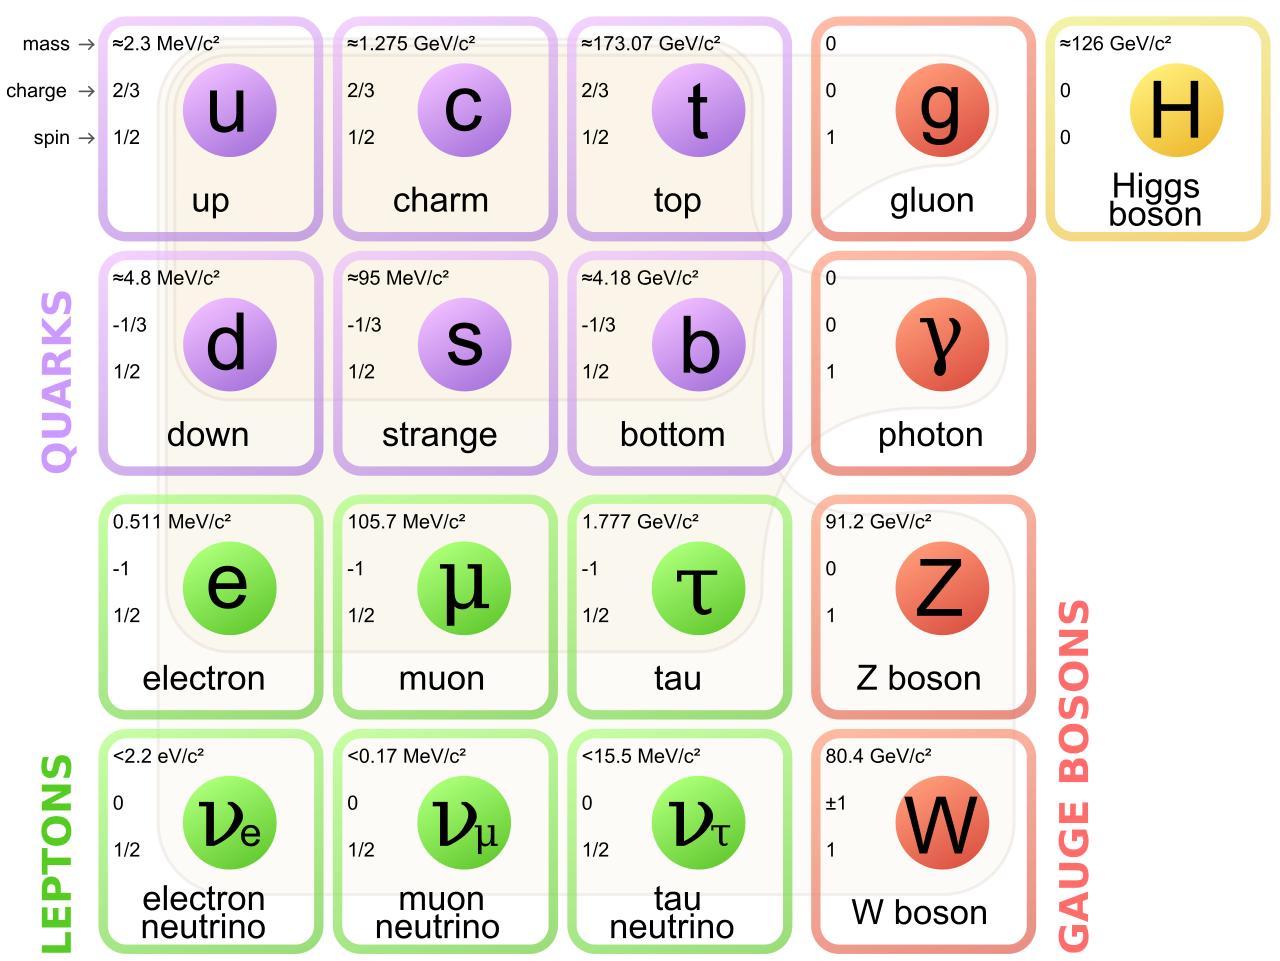
\includegraphics[width=0.8\linewidth]{../figures/images/standard_model.png}
\end{figure}
}

\addframe{Charmonium}{
Resonances formed by a $\qcharm\aqcharm$ pair: $\jpsi, \; \psip, \; \psipp, \; \ldots$
\additem{$\psip$ and $\psipp$ originally interpreted as excited states of $\jpsi$}
\additem{Evidence of mixed-states suggests more complicated picture}

\begin{figure}
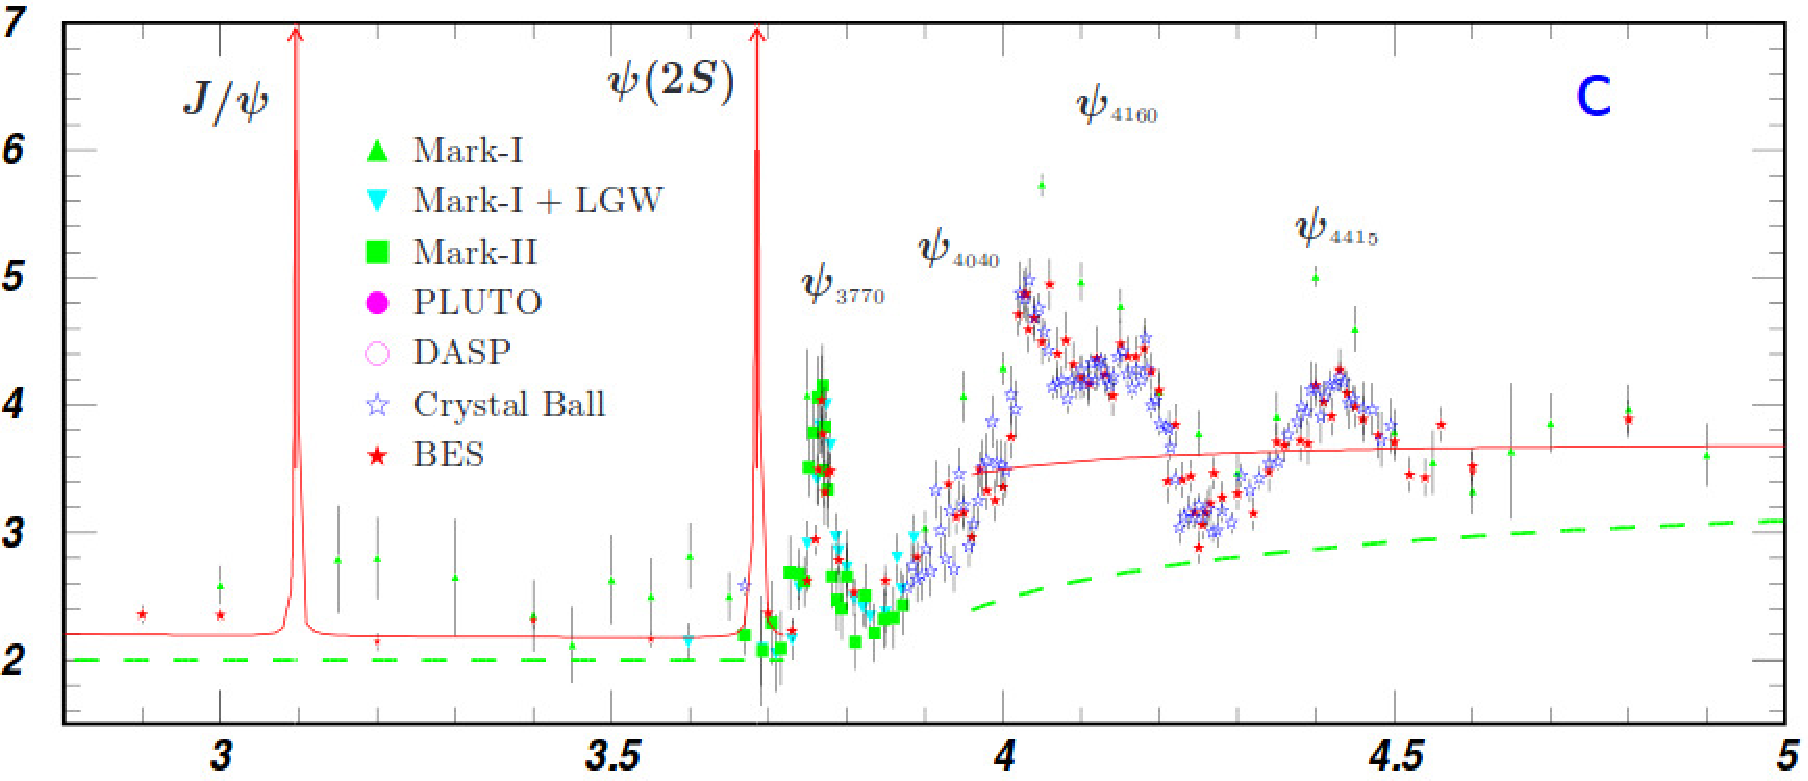
\includegraphics[width=\linewidth]{../figures/images/R_scan.pdf}
\end{figure}
}

\addframe{OZI Rule}{

\vspace{-1.0cm}

\begin{columns}

\column{.5\textwidth} % Left column and width
\addcenter{\textbf{$\psip$}}

\vspace{-0.5cm}

\begin{figure}
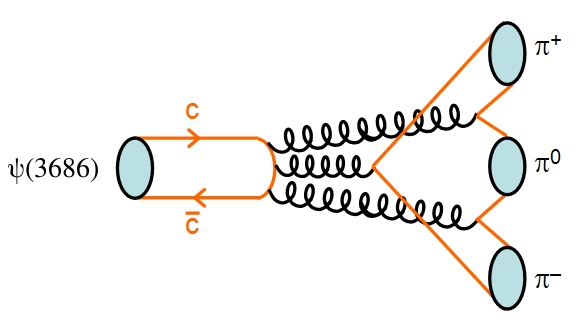
\includegraphics[width=\linewidth]{../figures/images/OZI_psip.png}
\end{figure}

\begin{itemize}
\item Requires three gluons for decay 

\item{Very narrow decay width
\additem{$\Gamma_{\psip} = \SI{0.286}{\MeV}$}}

\end{itemize}

\column{.5\textwidth} % Right column and width
\addcenter{\textbf{$\psipp$}}

\vspace{-0.3cm}

\begin{figure}
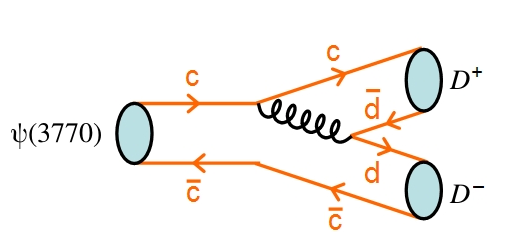
\includegraphics[width=\linewidth]{../figures/images/OZI_psipp.png}
\end{figure}

\vspace{0.35cm}

\begin{itemize}

\item Decays via open charm ($\DDbar$)

\item {Much wider decay width
\additem{$\Gamma_{\psipp} = \SI{27.5}{\MeV}$}}

\end{itemize}

\end{columns}

\vspace{0.3cm}

\addcenter{Addition of $\DDbar$ decays introduces drastically different behavior!}
}

\sectionframe{Accelerator and Detector}
% Show pictures of Beijing map and campus, if possible 

\addframe{Institute of High Energy Physics (IHEP)}{
\vspace{-0.3cm}

\addcenter{BESIII is hosted at the IHEP Campus located in Beijing, China}

\vspace{-0.3cm}

\begin{figure}
\includegraphics[width=\linewidth]{../figures/images/BESIII_layout.jpg}
\end{figure}
}

\addframe{Accelerator - Beijing Electron-Positron Collider II (BEPCII)}{

\begin{enumerate}

\item{Create positrons by firing electrons into stationary material
\additem{Generates high energy $\gamma$s which interact with material to form $\ee$}}

\item{Separate newly created positrons magnetically}

\item{Accelerate positrons in linear accelerator and feed into storage ring}

\item{Accelerate electrons and feed into the oppositely circulating ring
\additem{Electrons readily available, so extraction from photons unnecessary}}

\item{Focus each beam using magnets along storage rings until collision}

\end{enumerate}

\begin{figure}
\includegraphics[width=0.42\linewidth]{../figures/images/accelerator.jpg}
\hspace{1.5cm}
\includegraphics[width=0.42\linewidth]{../figures/images/storage_ring.jpg}
\end{figure}

}

\addframe{Detector - Beijing Spectrometer III (BESIII)}{
Collision of beams tuned to occur at central point of detector
\additem{Beams angled during collision to improve integrated luminosity}

\vspace{-0.3cm}

\begin{columns}

\column{.5\textwidth} % Left column and width

Four main subdetector systems:
\begin{itemize}
\item Main Drift Chamber
\item Time-of-Flight
\item Electromagnetic Calorimeter
\item Muon Identifier 
\end{itemize}

\vspace{-0.3cm}

\begin{figure}
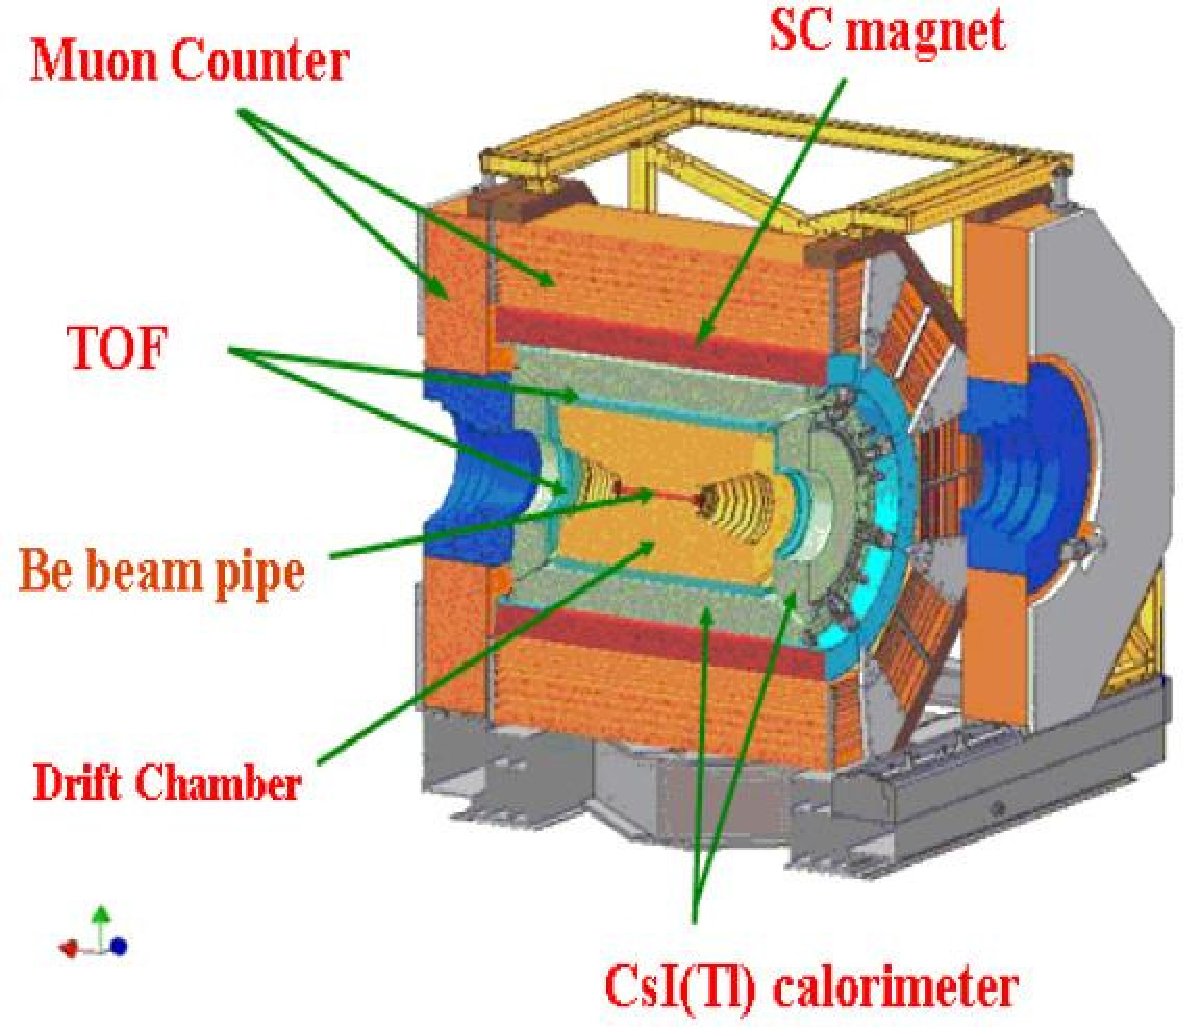
\includegraphics[width=0.85\linewidth]{../figures/images/detector.jpg}
\end{figure}

\column{.5\textwidth} % Right column and width

\begin{figure}
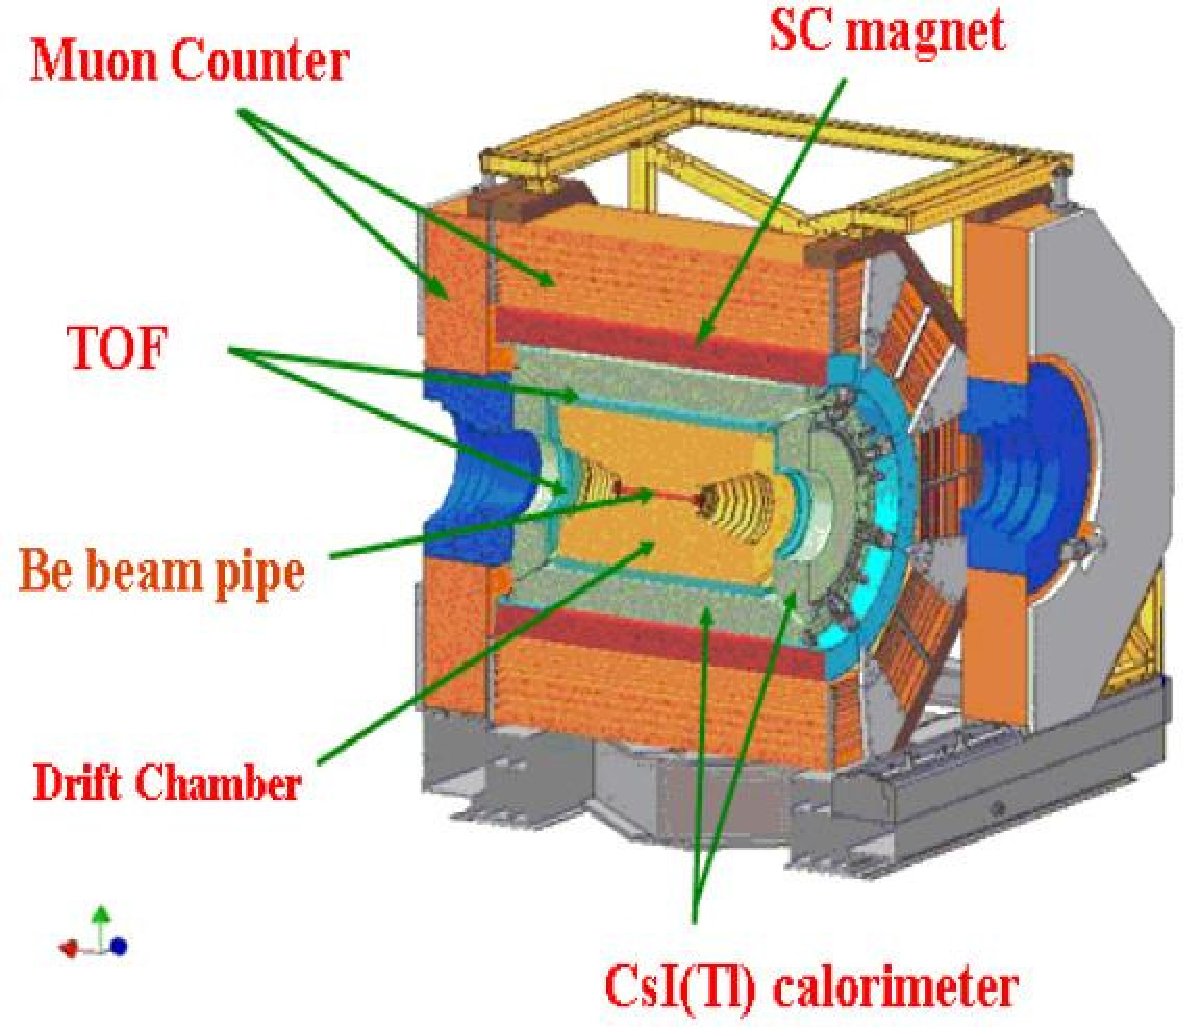
\includegraphics[width=\linewidth]{../figures/images/detector.pdf}
\end{figure}

\end{columns}

}

\addframe{Main Drift Chamber (MDC)}{
\vspace{-0.8cm}
\begin{columns}

\column{.55\textwidth} % Left column and width

\additem{Reconstruct charged tracks from interactions with sense wires (hits)
\additem{Wires surrounded by ionizable gas}
\additem{Initial ionization due to particle triggers avalanche of electrons}
\additem{High electric field near wires draws in released electrons to measure energy deposited}
}

\additem{Determine properties of particle from curvature in magnetic field
\additem{Radius determines momentum}
\additem{Direction determines charge}
}

\additem{Energy deposition rate ($\tdEdx$) helps determine particle candidate}


\column{.5\textwidth} % Right column and width

\addcenter{
BESIII Event Display

\begin{figure}
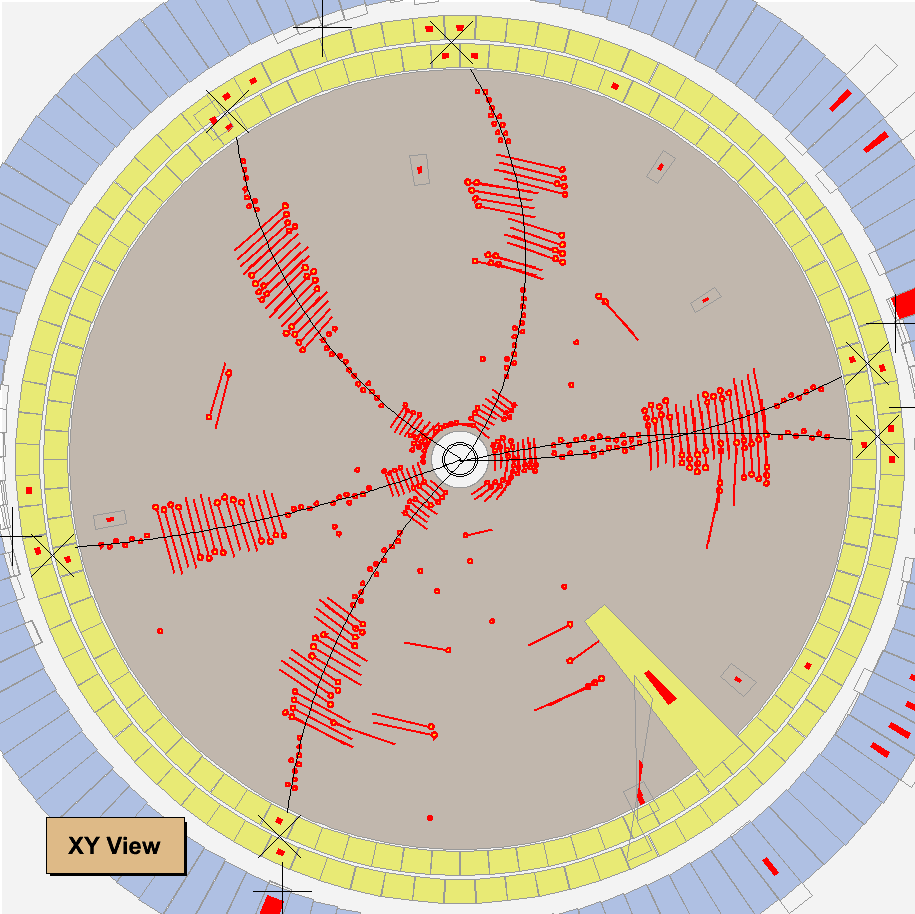
\includegraphics[width=\linewidth]{../figures/images/BESVis.png}
\end{figure}
}

\end{columns}
}

\addframe{Time-of-Flight (ToF)}{

\additem{Measure particle velocity using travel time after initial collision 
\additem{Scintillator bands located at \SIlist{0.81;0.86}{\m} from interaction point}
\additem{Attached to photomultiplier tubes to measure light output}
}

\additem{Helps distinguish between $\Kpm$ and $\pipm$ candidates at lower momenta
\additem{Combined with $\tdEdx$ measurements in MDC to set particle hypothesis}
}

\vspace{-0.6cm}

\begin{columns}

\column{0.5\textwidth} % Left column and width
\addcenter{MDC Measurements}

\vspace{-0.6cm}

\begin{figure}
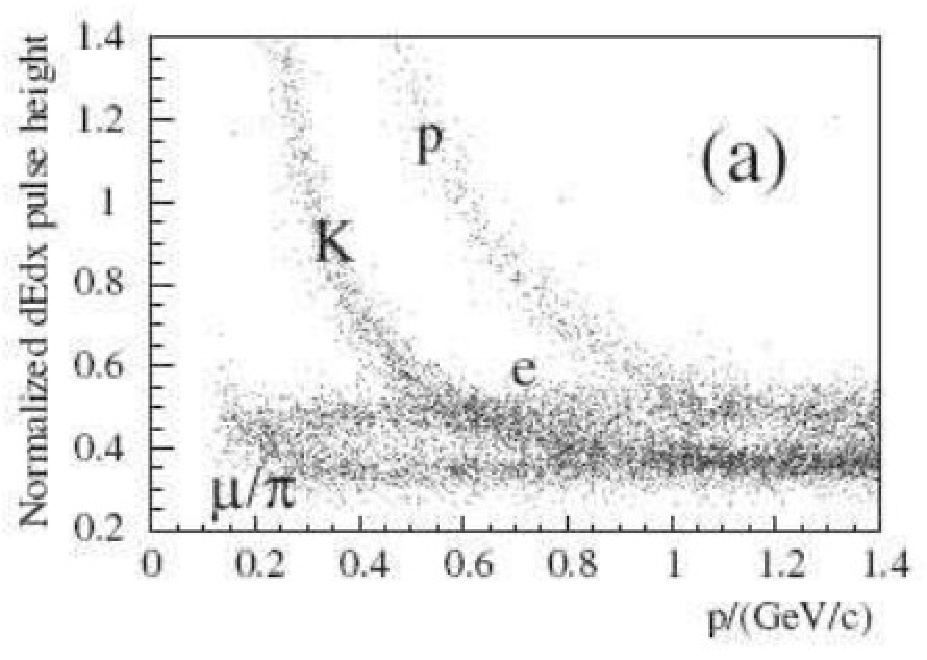
\includegraphics[width=\linewidth]{../figures/images/dEdx.pdf}
\end{figure}


\column{0.5\textwidth} % Right column and width
\addcenter{ToF Measurements}

\vspace{-0.6cm}

\begin{figure}
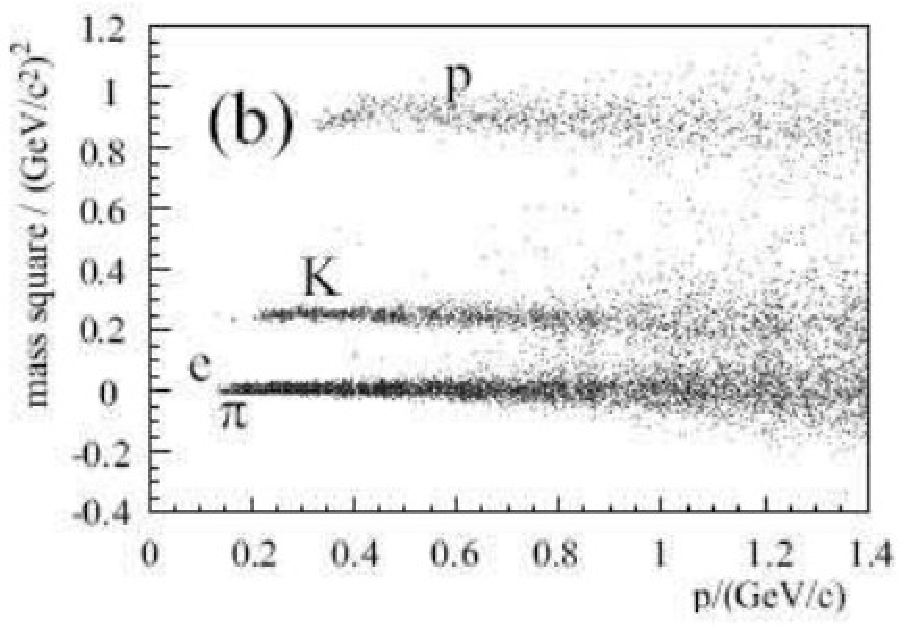
\includegraphics[width=\linewidth]{../figures/images/ToF.pdf}
\end{figure}

\end{columns}
}

\addframe{Electromagnetic Calorimeter (EMC)}{
\additem{Measure energy deposited by electron and photon tracks
\additem{Other particles are generally relativistic and thereby minimum ionizing
\additem{These deposit relatively constant energy, independent of momenta}
}
\additem{Use CsI(Tl) crystals attached to photodiodes to measure energy
\additem{Energy lost primarily in gaps of arrangement or out the back of crystals}
}
}
\additem{Allows reconstruction of purely neutral decays, such as $\piO \rightarrow \photon\photon$}

\begin{figure}
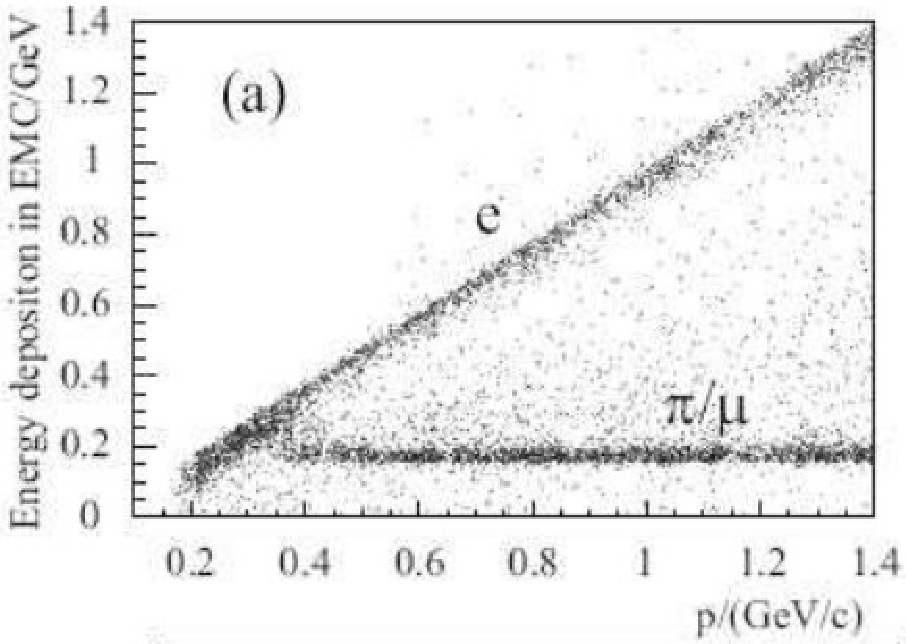
\includegraphics[width=0.5\linewidth]{../figures/images/EMC.pdf}
\end{figure}
}

\addframe{Muon Identifier (MUC)}{
\additem{Identify tracks traversing through multiple layers as muons
\additem{Most particle types will be stopped before reaching the MUC
\additem{Electrons susceptible to Bremsstrahlung radiation}
\additem{Kaons and pions susceptible to strong interactions}
}
\additem{Requires muons with $p > \SI{0.4}{\GeV}$ for appropriate curvature}
}

\begin{figure}
\includegraphics[width=0.5\linewidth]{../figures/images/muon.jpg}
\end{figure}
}

\addframe{Triggering System}{

\additem{Events filtered through two-step process
    \additem{L1: Hardware - Extracts information from various subdetectors
        \additem{MDC \\
            \qquad - Examines the number of superlayers each track passes through \\
            \qquad \qquad \textit{\scriptsize Superlayer: a collection of wires at same radial distance} \\
            \qquad - Applies a cut on minimum transverse momentum for each 
        }
        \additem{ToF \\
            \qquad - Examines number of hits in barrel and endcap regions \\
            \qquad - Checks for hits which are on opposite sides of the detector
        }
        \additem{EMC \\
            \qquad - Examines clustering of deposited energy around local maximum
        }
    }
    \additem{L3: Software - Assembles information to decide if potentially relevant}
}
\additem{Quickly and efficiently removes non-physics background events
\additem{e.g., reduces beam-related backgrounds from {$\sim$}\SI{13}{\MHz} to {$\sim$}\SI{1}{\kHz}}
}

}

\sectionframe{Analysis Software}{
% Show images of event display and... generic code? I dont know

\addframe{Monte Carlo Generation}{
\additem{Create simulations of detector construction and particle interactions
\additem{Model material composition and detector arrangement in GEANT4}
\additem{Simulate particle decay behavior using physics generators}
\additem{Generate decays which could be mistaken as $\DDbar$ in reconstruction \\
$\quad \ee \rightarrow \tautau, \quad \ee \rightarrow \ypsip, \quad \ee \rightarrow \qqbar, \quad \ldots$}
}
\additem{Process samples using BESIII Offline Software System (BOSS)
\additem{Use information gathered by subdetectors to reconstruct events} 
\additem{Extract relevant physical parameters ($\DeltaE, \; \mbc, \; \ldots$) from each}
}
\additem{Identify contributions of generated background samples seen in data
\additem{Process both data and Monte Carlo (MC) samples identically}
\additem{Subtract background components from data to determine signal events}
}
}

\addframe{$D$-Tagging}{

\begin{columns}

\column{0.6\textwidth} % Left column and width
\vspace{-0.6cm}

\additem{Reconstruct $D$ candidates from decays \\
\qquad $D \rightarrow \{\pipm, \; \Kpm, \; \piO, \; \Ks\}$
}

\additem{Modes selected based on \\ reconstruction efficiency
\additem{High branching fractions}
\additem{Manageable number of tracks (multiplicity)}
}

\additem{Search through track combinations for those matching reconstructed modes
\additem{Take best set per mode based on \\
\vspace{0.2cm}
$\DeltaE = |\Ebeam - \Etag|$ \\
\vspace{0.2cm}
$\mbc = \sqrt{\Ebeam^2 - |\ptag|^2}$
}
\additem{Allows multiple candidates per event}
}

\column{0.45\textwidth} % Right column and width
\vspace{-0.6cm}

\begin{table}[h]
\renewcommand\arraystretch{1.3}
\centering
\begin{tabular}{c l}
\multicolumn{2}{c}{Reconstructed Modes*} \\
\hline
(0) & $\DOmodeA$ \\
(1) & $\DOmodeB$ \\
(3) & $\DOmodeC$ \\
\hline
(200) & $\DpmodeA$ \\               
(201) & $\DpmodeB$ \\
(202) & $\DpmodeC$ \\
(203) & $\DpmodeD$ \\
(204) & $\DpmodeE$ \\               
(205) & $\DpmodeF$ \\               
\hline
\multicolumn{2}{c}{{\footnotesize *Charge conjugation implied}} \\
\end{tabular}
\end{table}

\end{columns}

}


\sectionframe{Measurement of the $\DDbar$ Cross Section}
% Show images of derivation formulas, energy measurements, fitting plots, cross sections, and systematics

\addframe{Procedure}{
Derive theoretical model used to describe cross section

List data samples used for measurement

Determine $\Ecm$ and $\lum$ for each data point

Identify signal and background components

Measure efficiency of reconstruction

Combine everything to determine cross section

Assess systematic uncertainties
}

\addframe{Derivation of $\xsecpsipptoDDbar$}{
\additem{Need to convert integral expression into measurable function 
\addcenter{$\sigma^{RC}_{\DDbar}(W) = \int
{\color{red} z_{\DDbar}(W \sqrt{1-x})} \,
{\color{blue} \sigma_{\DDbar}(W \sqrt{1-x})} \,
{\color{green2} \mathcal{F}(x, W^2)} \,
dx$}
\additem{${\color{red}z_{\DDbar}}$: Coulomb interaction ($\Dp\Dm$) and mass constraints}
\additem{${\color{blue}\sigma_{\DDbar}}$: Born level (lowest order) cross section}
\additem{${\color{green2}\mathcal{F}}$: Initial State Radiation (ISR) correction}
\additem{$x$: Approximation for fraction of energy radiated away}
}
\additem{Strategy: Split integral over $x$ into small intervals and sum results
\additem{Treat {\color{red}$z_{\Dp\Dm}$} and {\color{blue}$\sigma_{\DDbar}$} as constant in each interval
\additem{Use value at midpoint of interval for approximation}
}
\additem{Integrate simple function of ${\color{green2}\mathcal{F}(x, W^2)} = \beta \, x^{\beta - 1} F(W^2)$ over $x$}
\additem{Obtain complicated, but calculable function for $\DDbar$ cross section}
}
}

\addframe{Form Factors}{
\additem{Need to parameterize the {\color{orange}form factor} in the Born level cross section
    \addcenter{${\color{blue}\sigma_{\DDbar}(W)} = \frac{ \pi \alpha^2 }{ 3 W^2 } \beta_D^3 {\color{orange}|F_D(W)|^2}, \qquad \beta_D = \sqrt{1 - \frac{ 4 m_D^2 }{ W^2 } }$}
}
\additem{Comprised of resonant ($R$) and non-resonant ($NR$) components
    \addcenter{${\color{orange}F_D(W)} = F_D^{\text{NR}}(W) + \sum\limits_r F^{R_r}_D(W) \, e^{i \phi_r }$}
}
\additem{Resonant components parametrized by Breit-Wigner shape
    \addcenter{$F^R_D(W) = \frac{ 6 \, W \sqrt{ (\Gamma_{ee} / \alpha^2 ) ( \Gamma_{\DDbar}(W) / \beta^3_D ) } }{ M^2 - W^2 - i M \Gamma(W)}, \qquad \Gamma_{\DDbar}(W) = \Gamma(W) \times \BDD$}
}
\additem{Non-resonant component has no definitive parametrization 
\additem{Investigate two potential models for analysis
\additem{Exponential: generic form to approximate shape}
\additem{Vector Dominance Model (VDM): physically based parameters}
}
}
}

\addframe{Form Factor Models}{
\begin{columns}

\column{0.45\textwidth} % Left column and width
\vspace{-0.6cm}
\addcenter{\textbf{Exponential Model}}
\addcenter{$F_D^{NR} = \FNR \, \exp ( -q_D^2 / \aNR^2 )$}
\additem{Fit Parameters
\additem{$\FNR$: Amplitude}
\additem{$\aNR$: Width}
}
\additem{Used for systematic check}

\column{0.6\textwidth} % Right column and width
\vspace{-0.6cm}
\addcenter{\textbf{Vector Dominance Model}}
\addcenter{$F_D^{NR}(W) = F_D^{\psip}(W) + F_0$}
\additem{Fit Parameters
\additem{$\Gpsip$: Decay width for $\psip$*}
\additem{$F_0$: Higher resonances ($\psi(4040)$)}
}
\additem{Used for final results}
\additem{Use $\Mpsipp$ in place of $\Mpsip$
\additem{Avoid mass below $\DDbar$ threshold}
\additem{*Unclear physical meaning}
}

\end{columns}
}

\addframe{Data Samples}{
\additem{Use scan data to determine overall cross section shape
\additem{Taken over an energy range of \SIrange{3.643}{3.890}{\GeV}}
\additem{Split into 34 bins based on measurements of $\Ecm$}
\additem{Luminosity measured using $\ee \rightarrow \ee(\gamma)$ events ($\lum = \SI{69.80}{\invpb}$)}
\additem{Chosen to be above $\DO\aDO$ threshold and below $D^{*0}\aDO$ threshold}
\additem{Includes two bins below $\Dp\Dm$ threshold which have zero production}
}
\additem{Use additional high statistics samples for comparison measurements
\begin{table}
\renewcommand\arraystretch{1.1}
\centering
\begin{tabular}{c|c|r}
Name & $\Ecm$ [\si{\GeV}] & \multicolumn{1}{c}{$\lum$} \\
\hline
On-Peak $\psipp^\dagger$ & 3.773 & \SI{2.93}{\invfb} \\
$XYZ$-Scan & 3.810 & \SI{50.54}{\invpb} \\
$R$-Scan & 3.850 & \SI{7.95}{\invpb} \\
\hline
\multicolumn{3}{l}{\footnotesize $^\dagger$Analysis of $\DDbar$ cross section performed independently}
\end{tabular}
\end{table}
}
}

\addframe{Center-of-Mass Energy}{
\addcenter{\textbf{Accurate $\Ecm$ required for precise determination of $\Mpsipp$}}
\additem{Measure $\Ecm$ using $M_{\text{inv}}$ of `On-Peak $\psipp$' $\ee \rightarrow \mumu$ events}
\additem{Compare results to separate, trustworthy procedure using $\DDbar$ events
\additem{Difference in average values determines correction to $\mumu$ procedure}
}
\additem{Measure $\Ecm$ for scan data using $\mumu$ procedure
\additem{Shift values by correction from $\DDbar$ procedure to get final results}
}

\begin{figure}
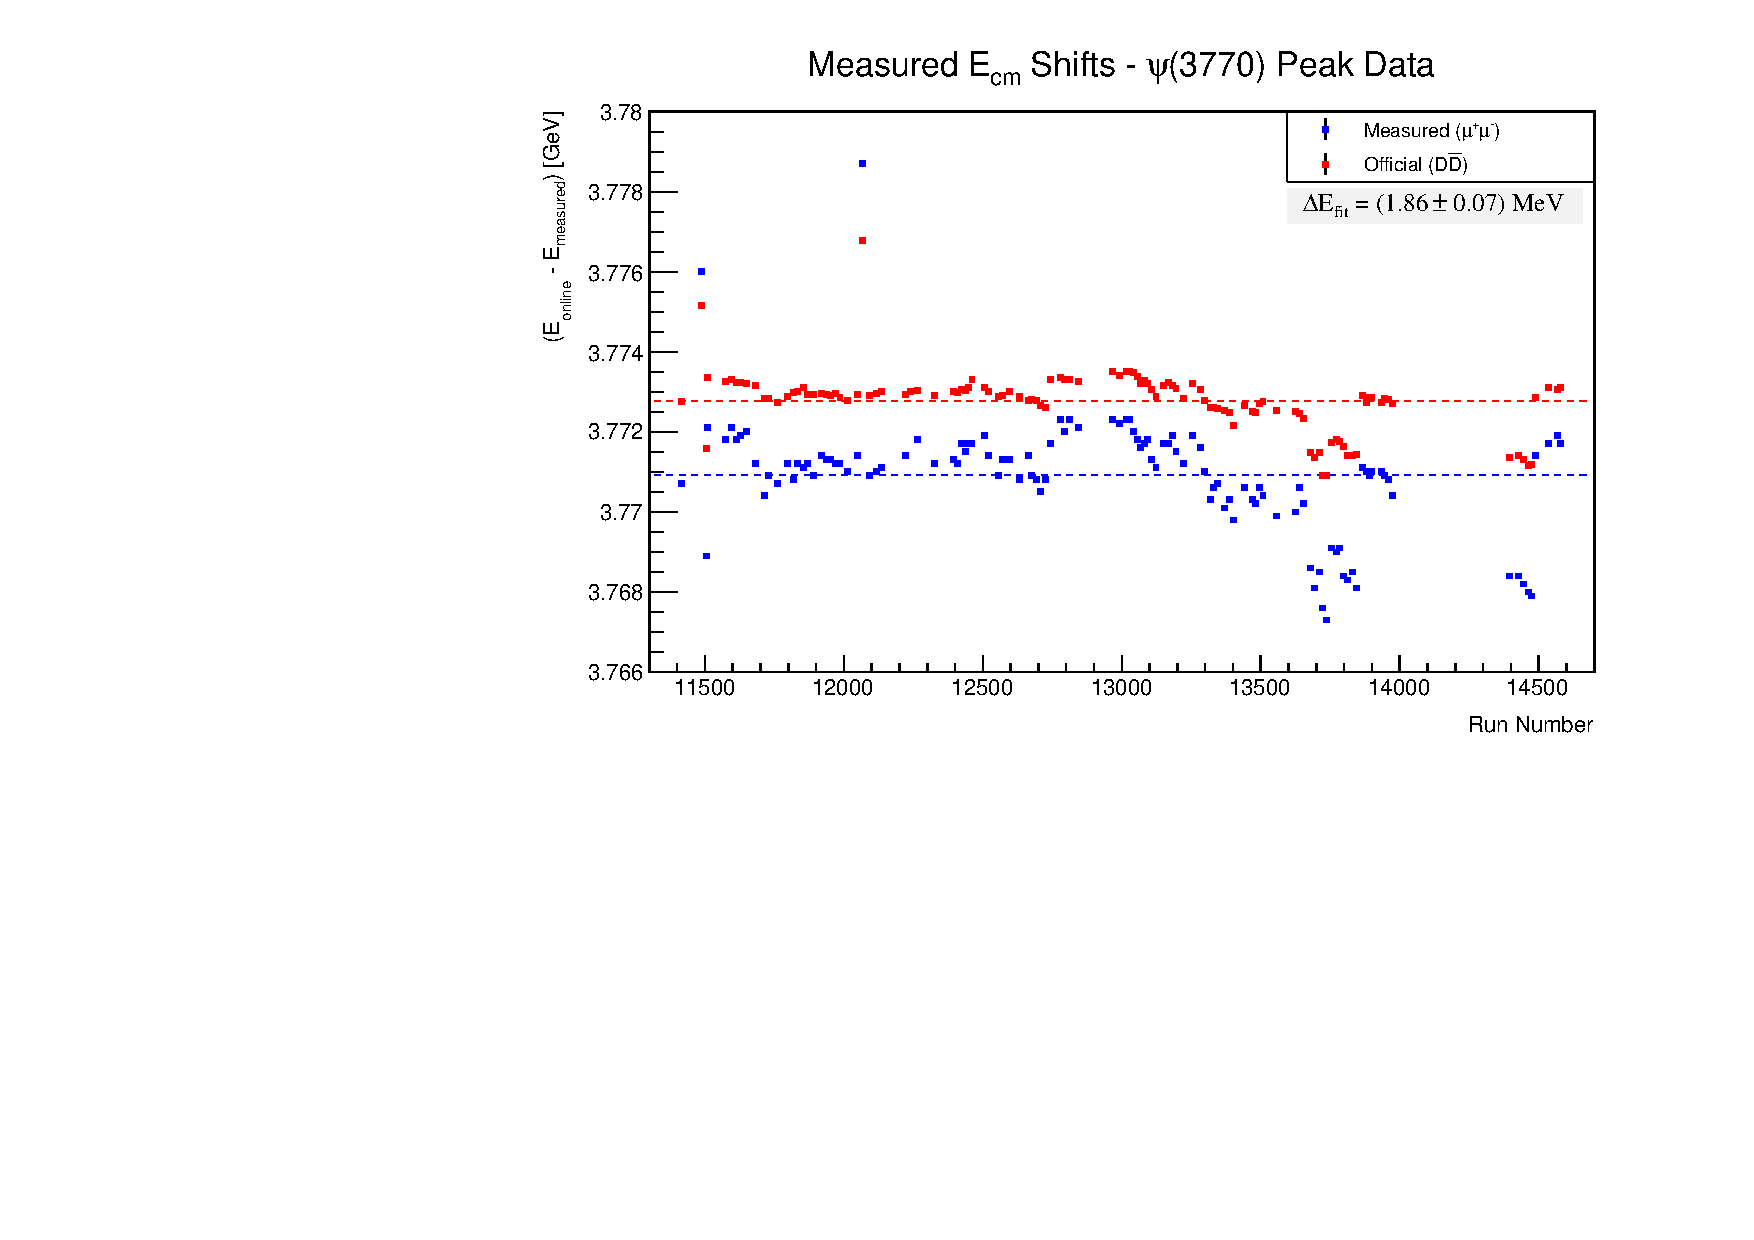
\includegraphics[width=0.5\linewidth]{../figures/plots/E_cm_fit_cut_new.pdf}
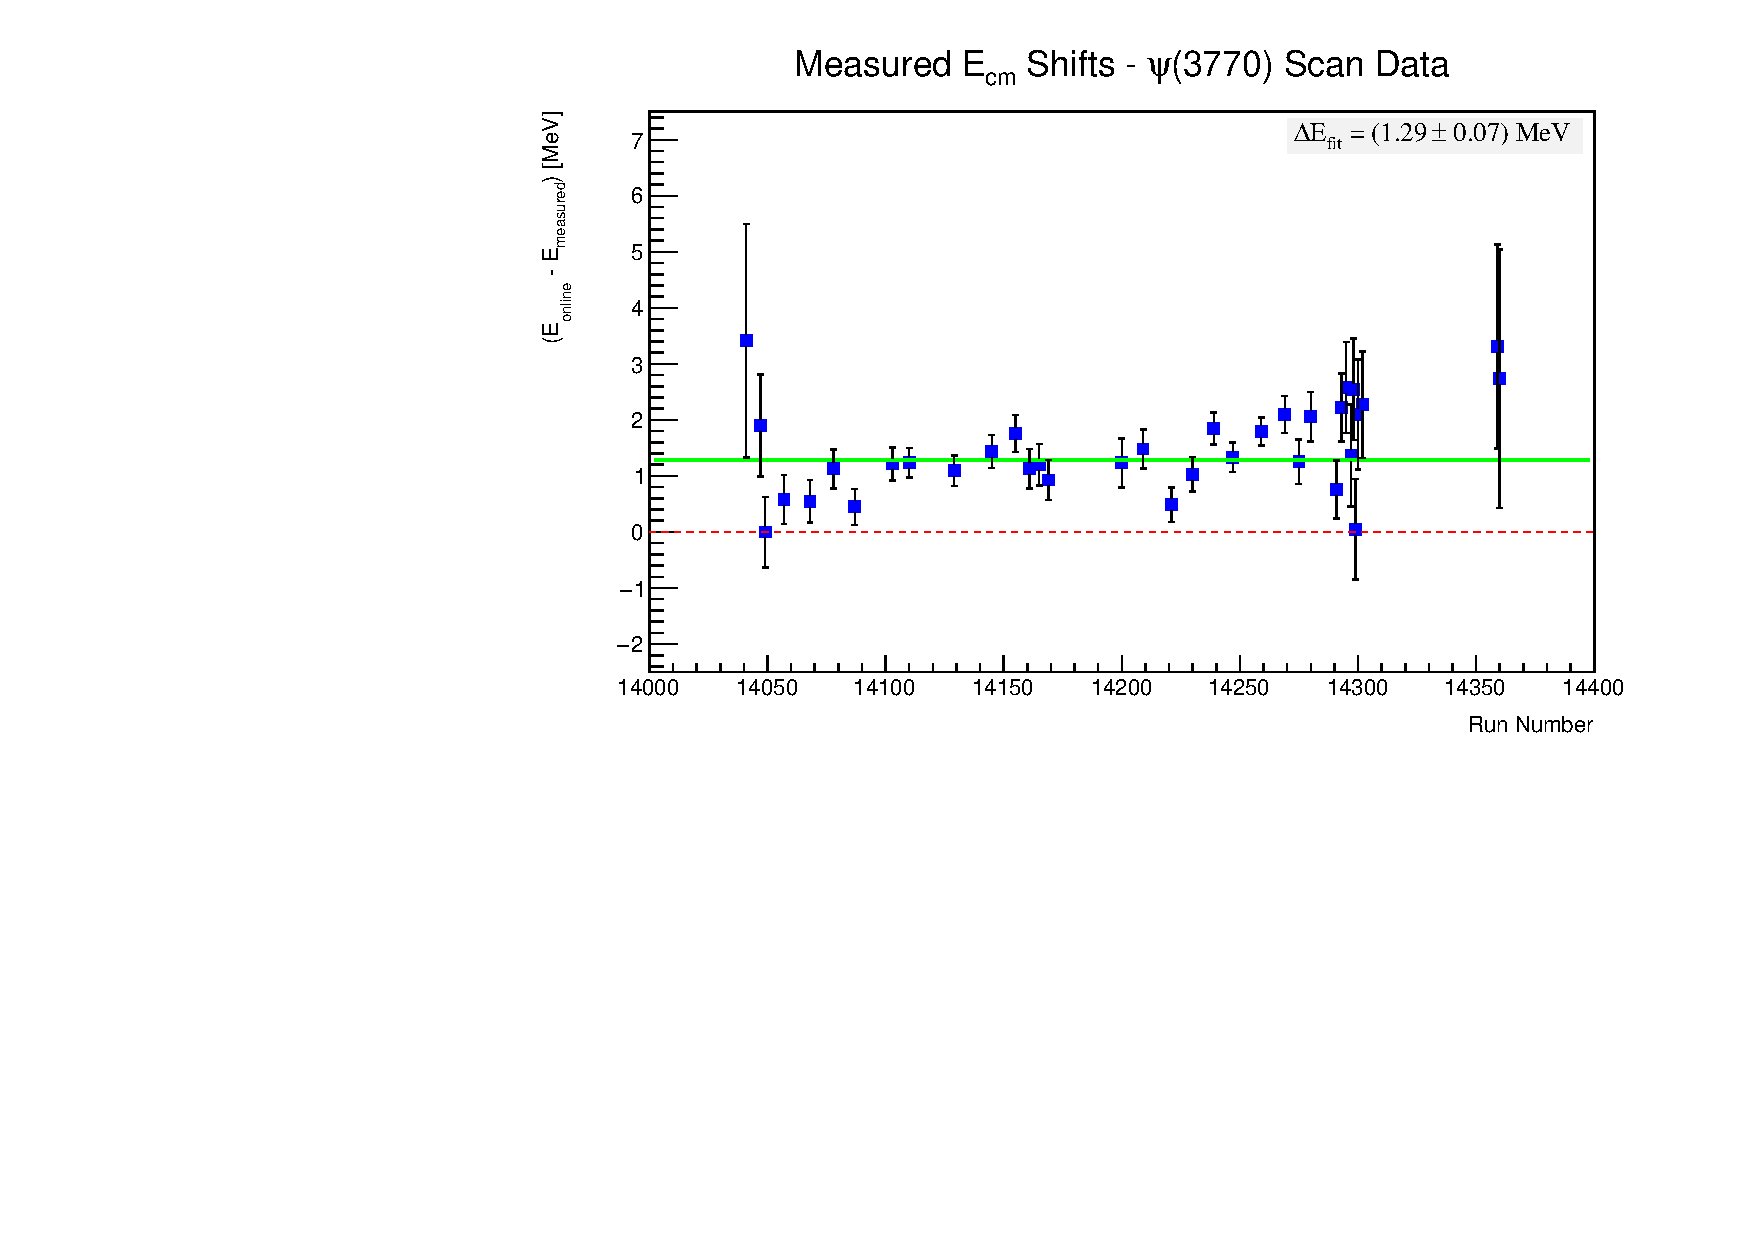
\includegraphics[width=0.5\linewidth]{../figures/plots/E_cm_shifts_scan_fit_cut_new.pdf}
\end{figure}
}

\addframe{Monte Carlo Generation}{
\additem{Generate MC samples to help identify signal and background rates
\additem{Signal: $\qquad \qquad \psipp \rightarrow \DO\aDO, \qquad \psipp \rightarrow \Dp\Dm$}
\additem{Background: $\qquad \quad \qqbar, \quad \tautau, \quad \yjpsi, \quad \ypsip$}
\additem{Events per sample of ${\sim}10^6$-$10^7$ depending on decay type}
\additem{Decays simulated using run-dependent $\Ecm$ and accelerator conditions}
}

\vspace{0.7cm}

\additem{Samples of $\psipp \rightarrow \DDbar$ generated using our cross section results 
\additem{Use Born cross section from final fit results to improve MC generator}
\additem{Requires iteration of MC generation to properly reflect true shape
\additem{Performed 5 iterations of input shapes for analysis}
}
}
}

\addframe{Signal Determination}{
\additem{Measure $\DO\aDO$ / $\Dp\Dm$ yields separately with 2D fit
\additem{Use $D$-tagging code to identify candidates in each sample (data / MC)}
\additem{Extract $\DeltaE$ and $\mbc$ distributions and arrange MC samples into groups \\
\begin{columns}
\column{0.45\textwidth} % Left column and width
\hspace{1.3cm} (1) Proper $D$-tags \\
\hspace{1.3cm} (2) Improper $D$-tags

\column{0.45\textwidth} % Right column and width
(3) $\qqbar$ \\
(4) $\tautau + \yjpsi + \ypsip$
\end{columns}
}
\additem{Float normalizations of each group to match data distributions ($\chi^2$)}
}
\begin{figure}
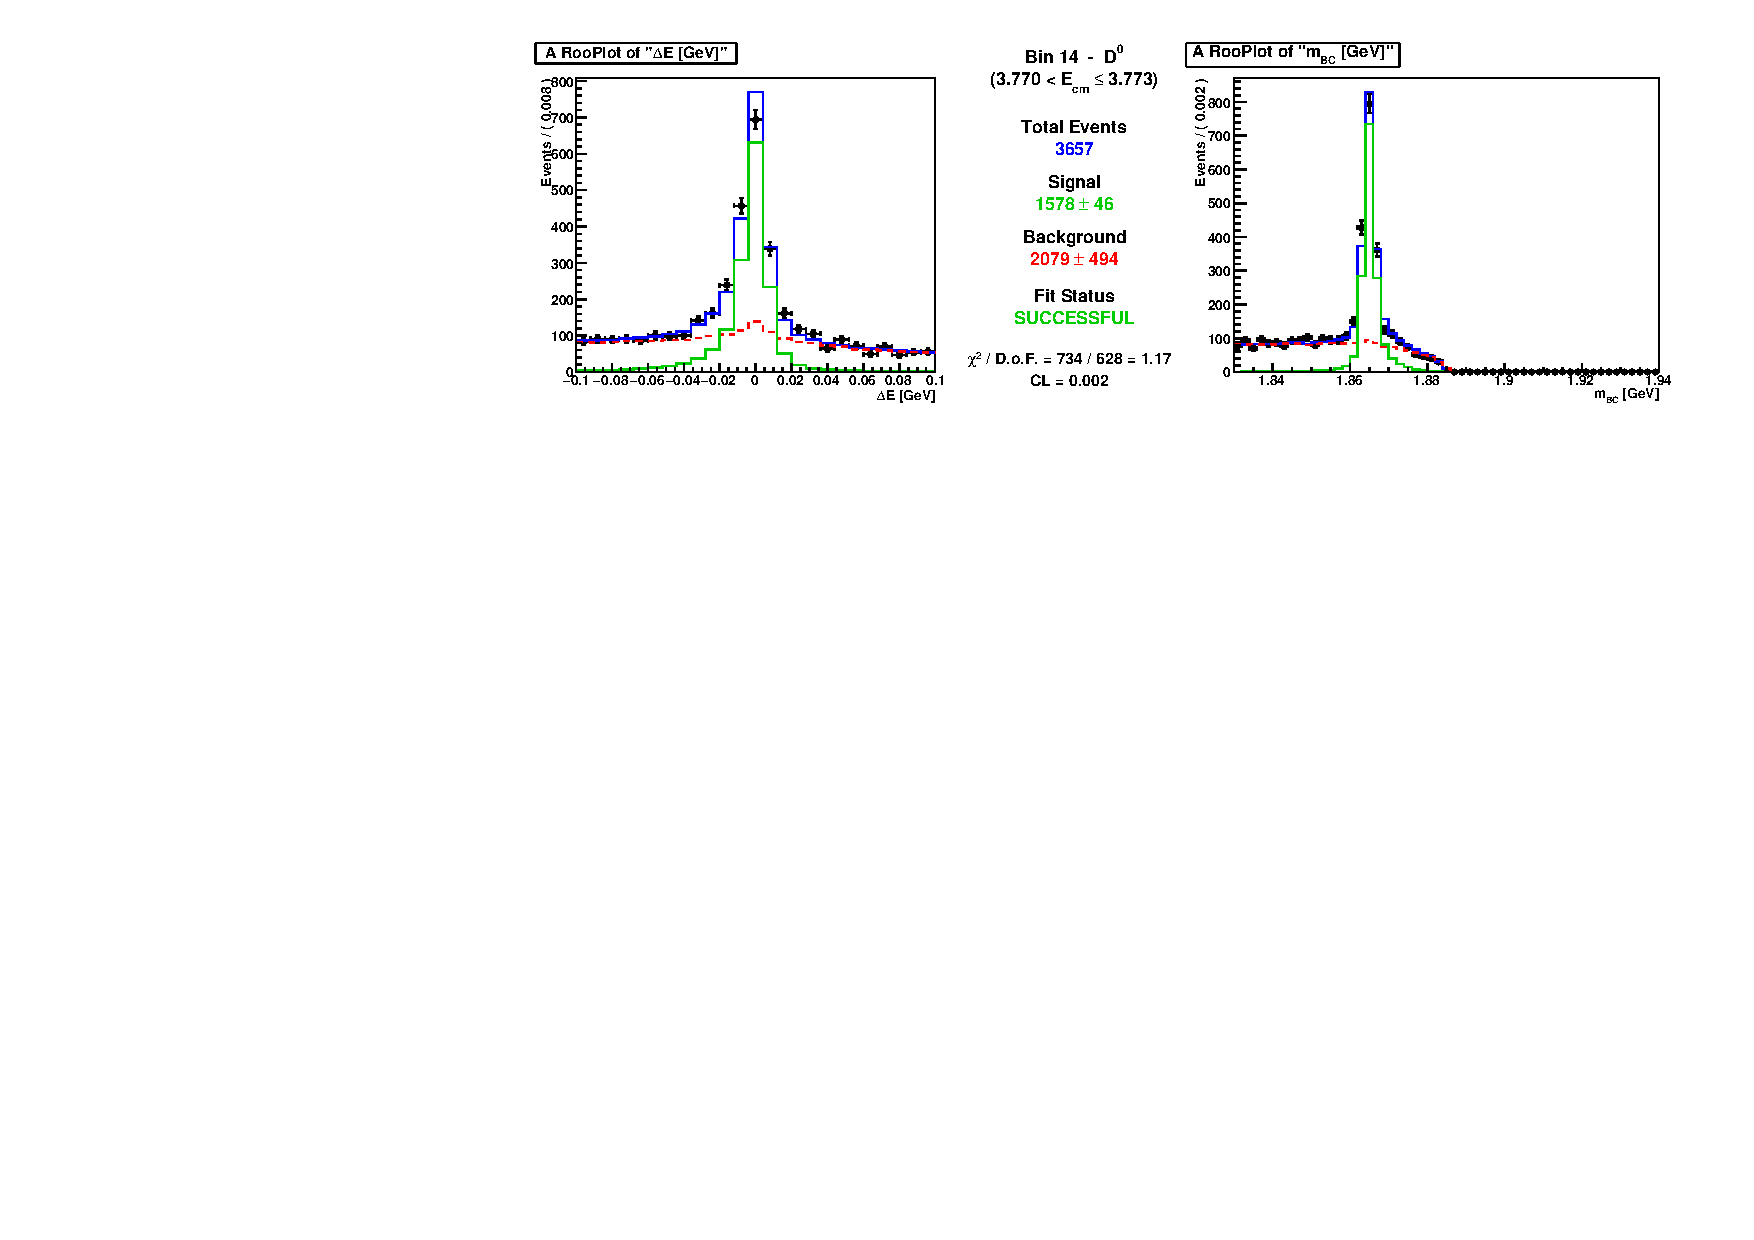
\includegraphics[width=\linewidth]{../figures/plots/fit_results/D0_bin_14.pdf}
\end{figure}
}

\addframe{Efficiency Correction}{
\additem{Correct for $D$ reconstruction efficiency to determine total production
\additem{Average MC candidate amounts ($N_{\text{prop}}$ vs. $N_{\text{gen}}$) over decay modes}
\addcenter{$\epsilon_{D} = \sum\limits_i \epsilon_{i \text{ rec}} \, \mathcal{B}_i = \sum\limits_i \left( \frac{ N_{i \text{ prop}} }{ N_{i \text{ gen}} } \right) \mathcal{B}_i$}
}

{\footnotesize
\begin{table}
\centering
\begin{tabular}{l r@{$\; \pm \;$}l r@{$\; \pm \;$}l}
\hline
Decay Mode ($i$) & \multicolumn{2}{c}{PDG $\mathcal{B}_i$ [\%]} & \multicolumn{2}{c}{MC Efficiency $\epsilon_{i \text{ rec}}$} \\
\hline
$\DOmodeA$ &  3.89 & 0.05 & 0.7002 & 0.0011 \\
$\DOmodeB$ & 13.93 & 0.50 & 0.3794 & 0.0004 \\
$\DOmodeC$ &  8.11 & 0.21 & 0.3988 & 0.0006 \\
\hline
\multicolumn{5}{c}{$\epsilon_{\DO} = (11.245 \pm 0.020)\%$} \\[1pt]
\hline
$\DpmodeA$ &  9.13 & 0.19 & 0.5471 & 0.0007 \\
$\DpmodeB$ &  5.99 & 0.18 & 0.2739 & 0.0006 \\
$\DpmodeC$ &  1.47 & 0.07 & 0.3883 & 0.0014 \\
$\DpmodeD$ &  6.99 & 0.27 & 0.2079 & 0.0005 \\
$\DpmodeE$ &  3.12 & 0.11 & 0.2237 & 0.0007 \\
$\DpmodeF$ &  0.95 & 0.03 & 0.4317 & 0.0018 \\
\hline
\multicolumn{5}{c}{$\epsilon_{\Dp} = (9.770 \pm 0.063)\%$} \\[1pt]
\hline
\end{tabular}
\end{table}
}
}

\addframe{Cross Section Fitting}{
\additem{Use signal amount, efficiency, and luminosity to find cross sections:
\additem{Include factor of 2 to correct for double counting ($D$ vs. $\DDbar$)}
}
\addcenter{$\sigma_{\DDbar}^{RC}(E_i) = \frac{ N_D(E_i) }{ 2 \, \epsilon_D(E_i) \, \mathcal{L}(E_i) }$}

\additem{Fit to theoretical formulation to determine $\psipp$ parameters
\additem{$\Mpsipp \qquad \Gpsipp \qquad \GeepsipptoDDbar \qquad \Ppsipp$}
\additem{Use $\GeepsipptoDDbar$ in place of known $\BnDD$ or $\Geepsipp$}
}
\additem{Two additional fit parameters depending on form factor choice
\additem{Exponential: $\quad \FNR \qquad \aNR \qquad \qquad$ VDM: $\quad \Gpsip \qquad F_0$}
}
\additem{Minimize sum of $\chi^2$ distributions for $\DO$ and $\Dp$}
}

\addframe{Exponential Results}{
\begin{figure}
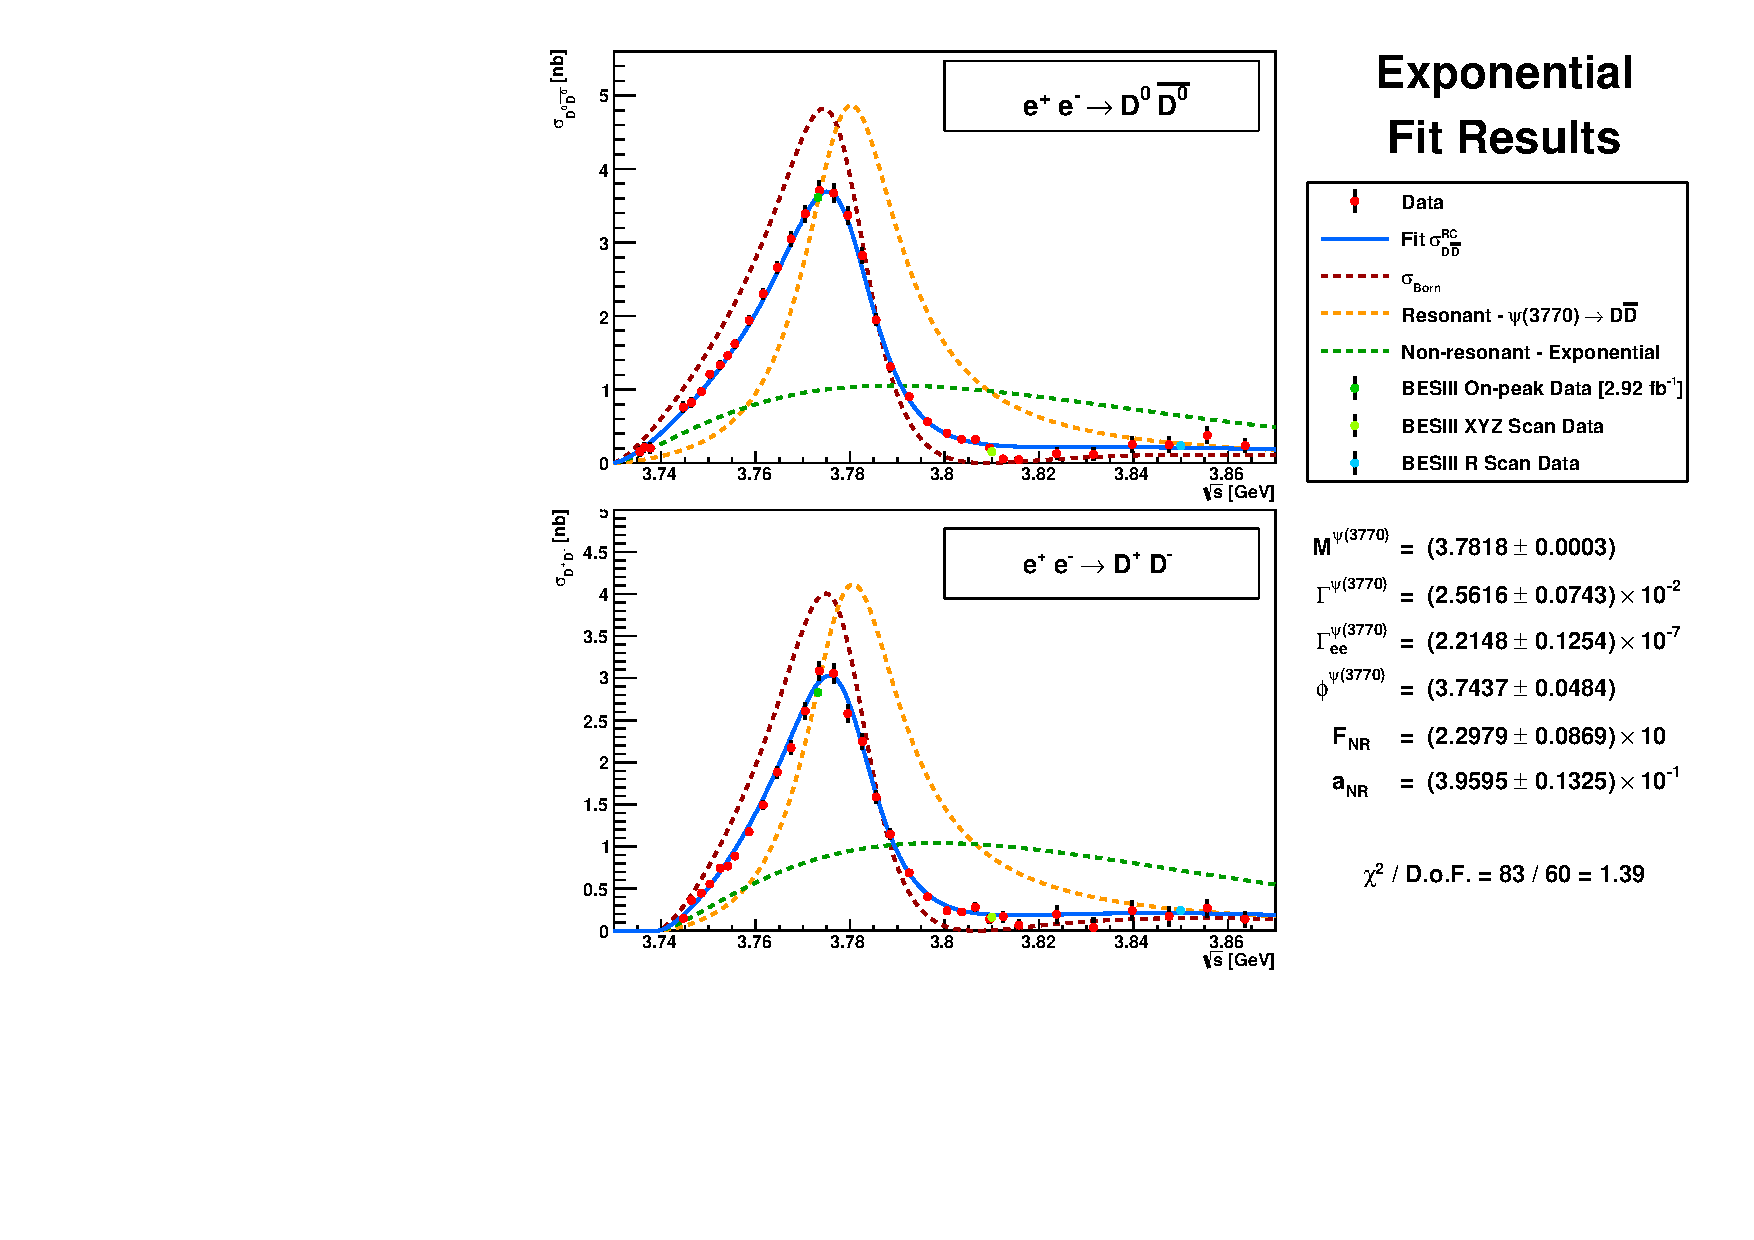
\includegraphics[scale=0.47]{../figures/plots/lineshape_exp.pdf}
\end{figure}
}

\addframe{Vector Dominance Model Results}{
\begin{figure}
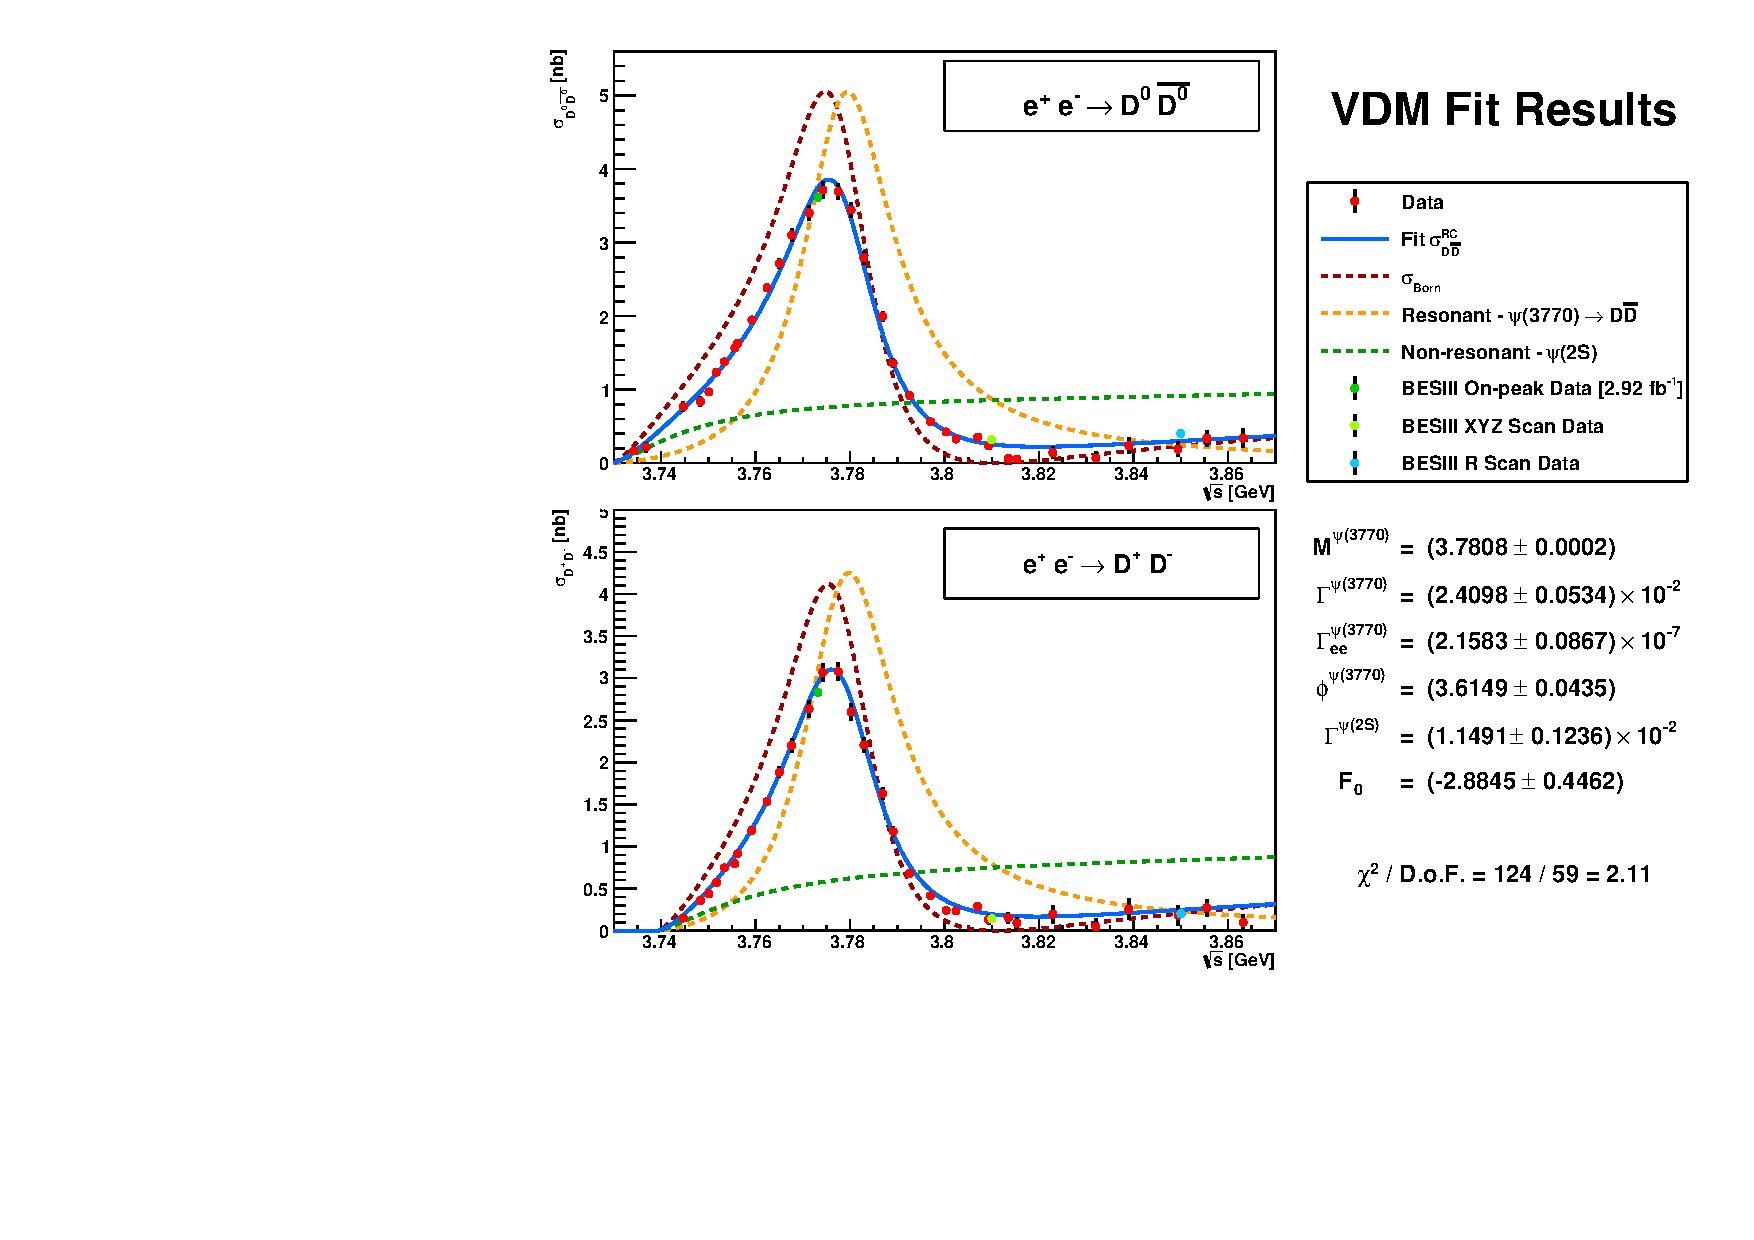
\includegraphics[scale=0.47]{../figures/plots/lineshape_vdm.pdf}
\end{figure}
}

\addframe{Results Overview}{
\additem{Both form factor choices show generally good agreement
\additem{Excess in $\chi^2$ largely due to two $\DO$ points just above \SI{3.81}{\GeV}}
\additem{Could indicate need for improved model in higher energy region}
}
\additem{Values for $\psipp$ parameters primarily dependent on peak region
\additem{Consistent shape in this region emphasizes quality of results}
}
\additem{Inteference related to behavior of Born level cross section
\additem{Reappearance of Born level events is strong indication of interference}
\additem{Impossible to reproduce with two non-interfering Breit-Wigner shapes}
}
}

\addframe{Born Level Event Contribution in $\mbc$}{
\begin{figure}
{\small \hspace{-0.5cm} At $\psipp$ Peak \hspace{2cm} Approaching Born Minimum}
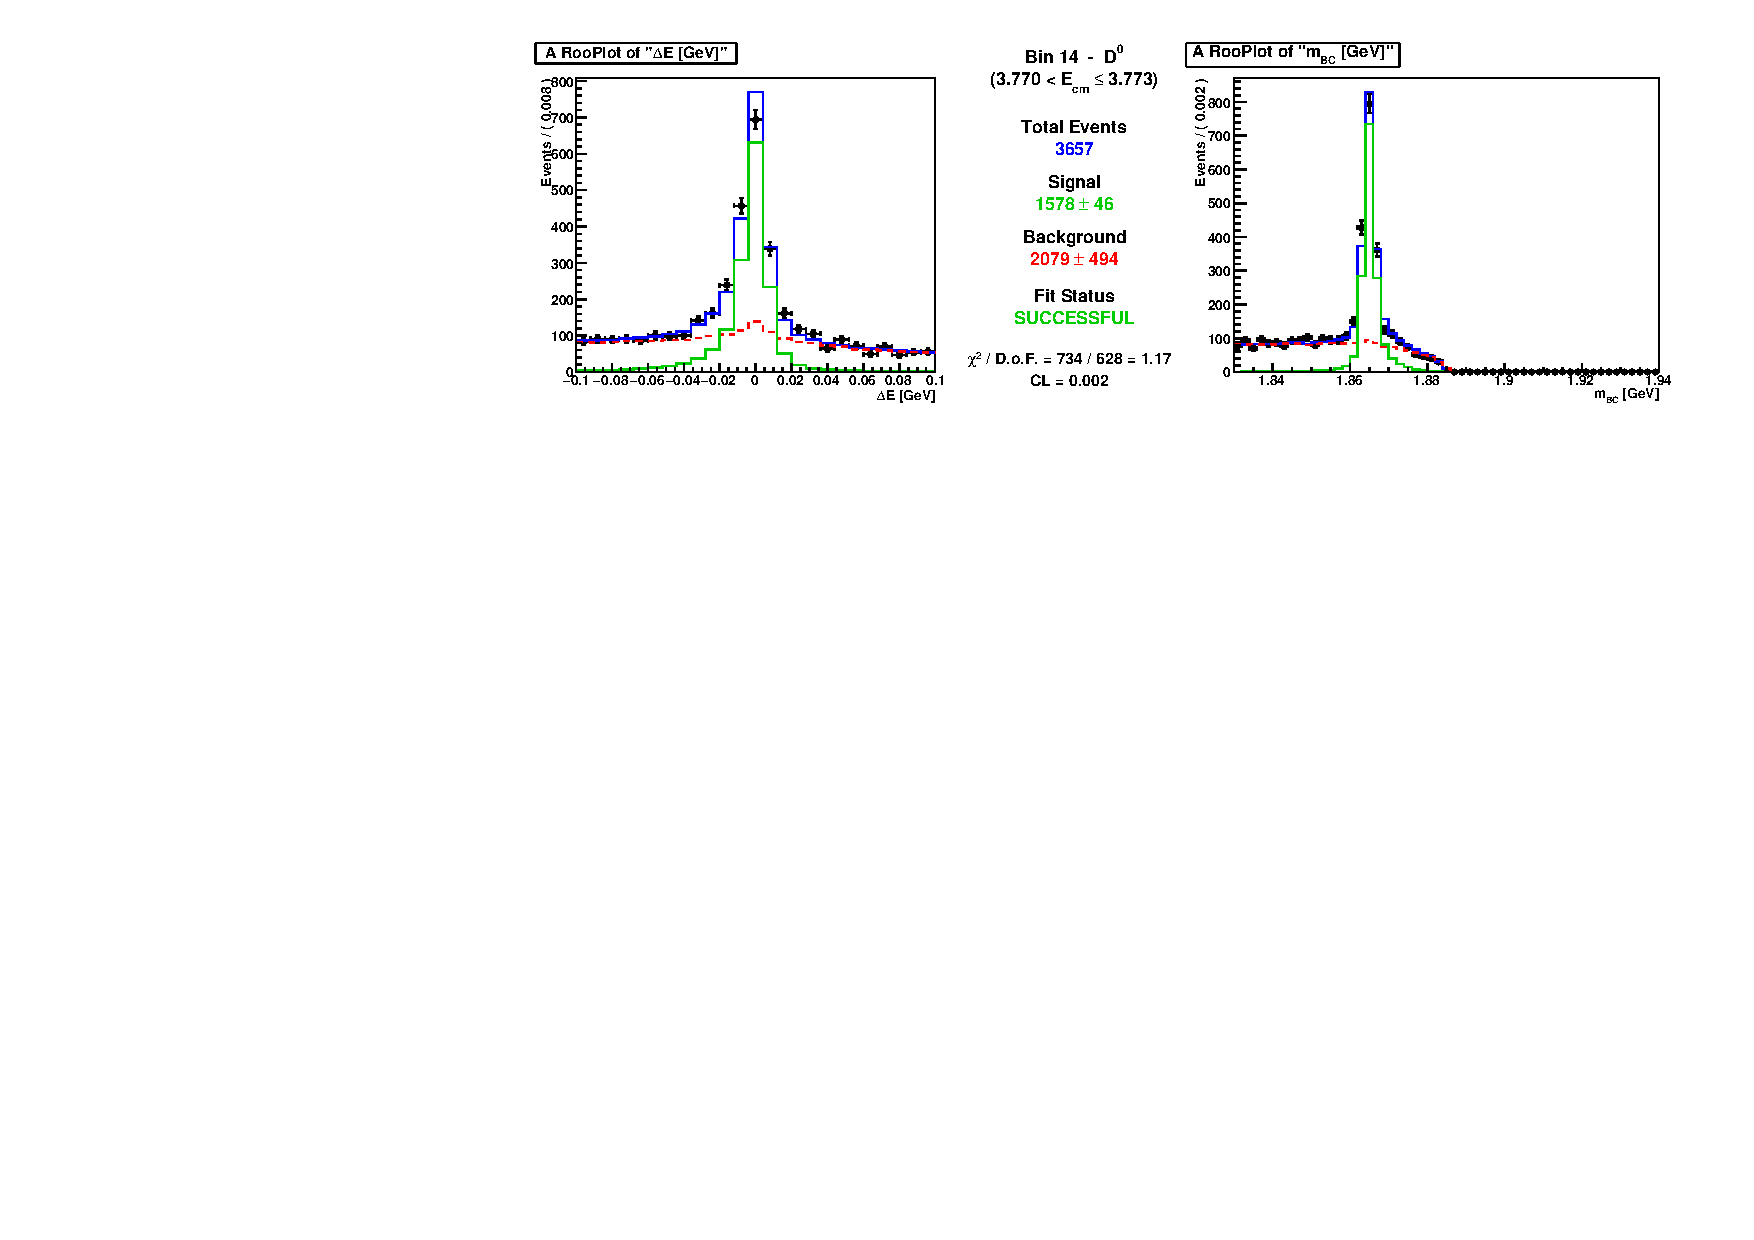
\includegraphics[trim={12cm 0 0 0},clip,width=0.3\linewidth]{../figures/plots/fit_results/D0_bin_14.pdf}
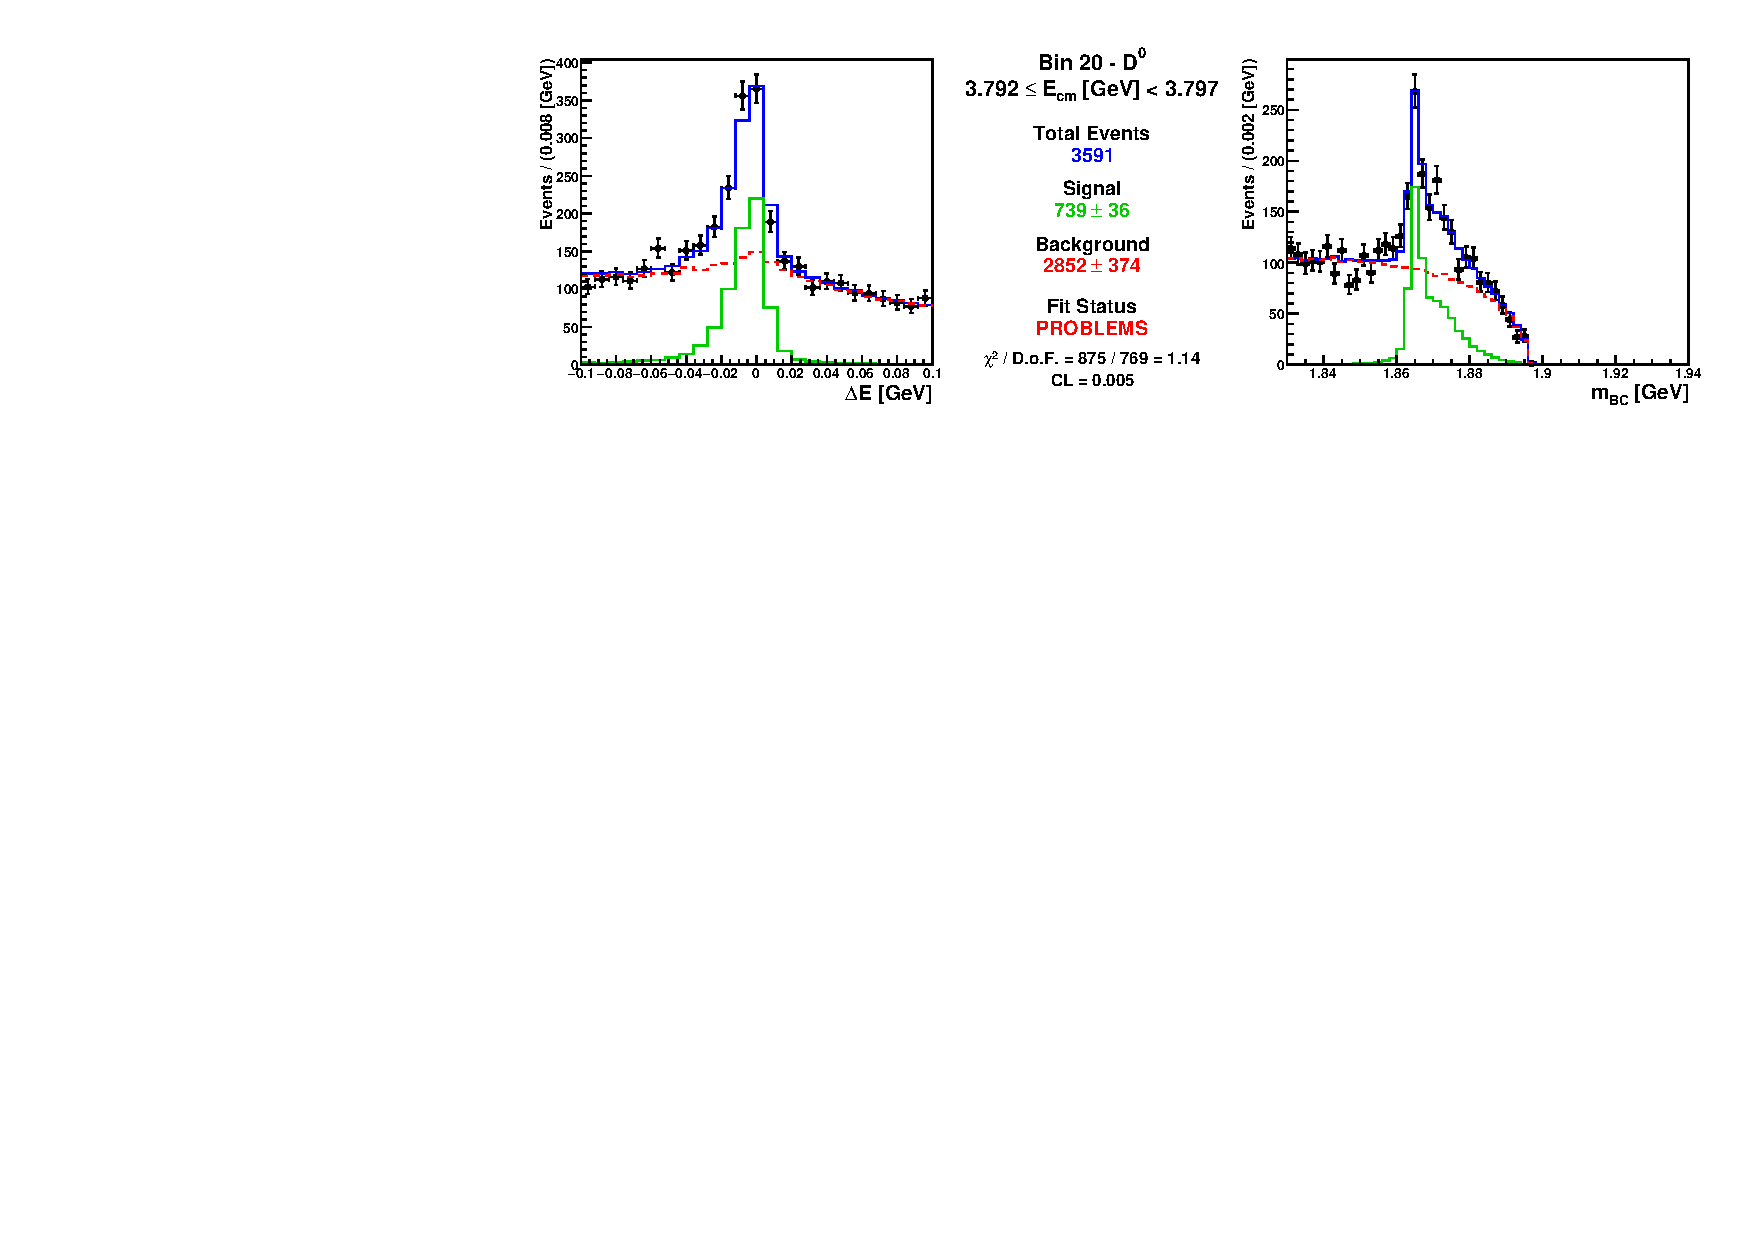
\includegraphics[trim={12cm 0 0 0},clip,width=0.3\linewidth]{../figures/plots/fit_results/D0_bin_20.pdf}
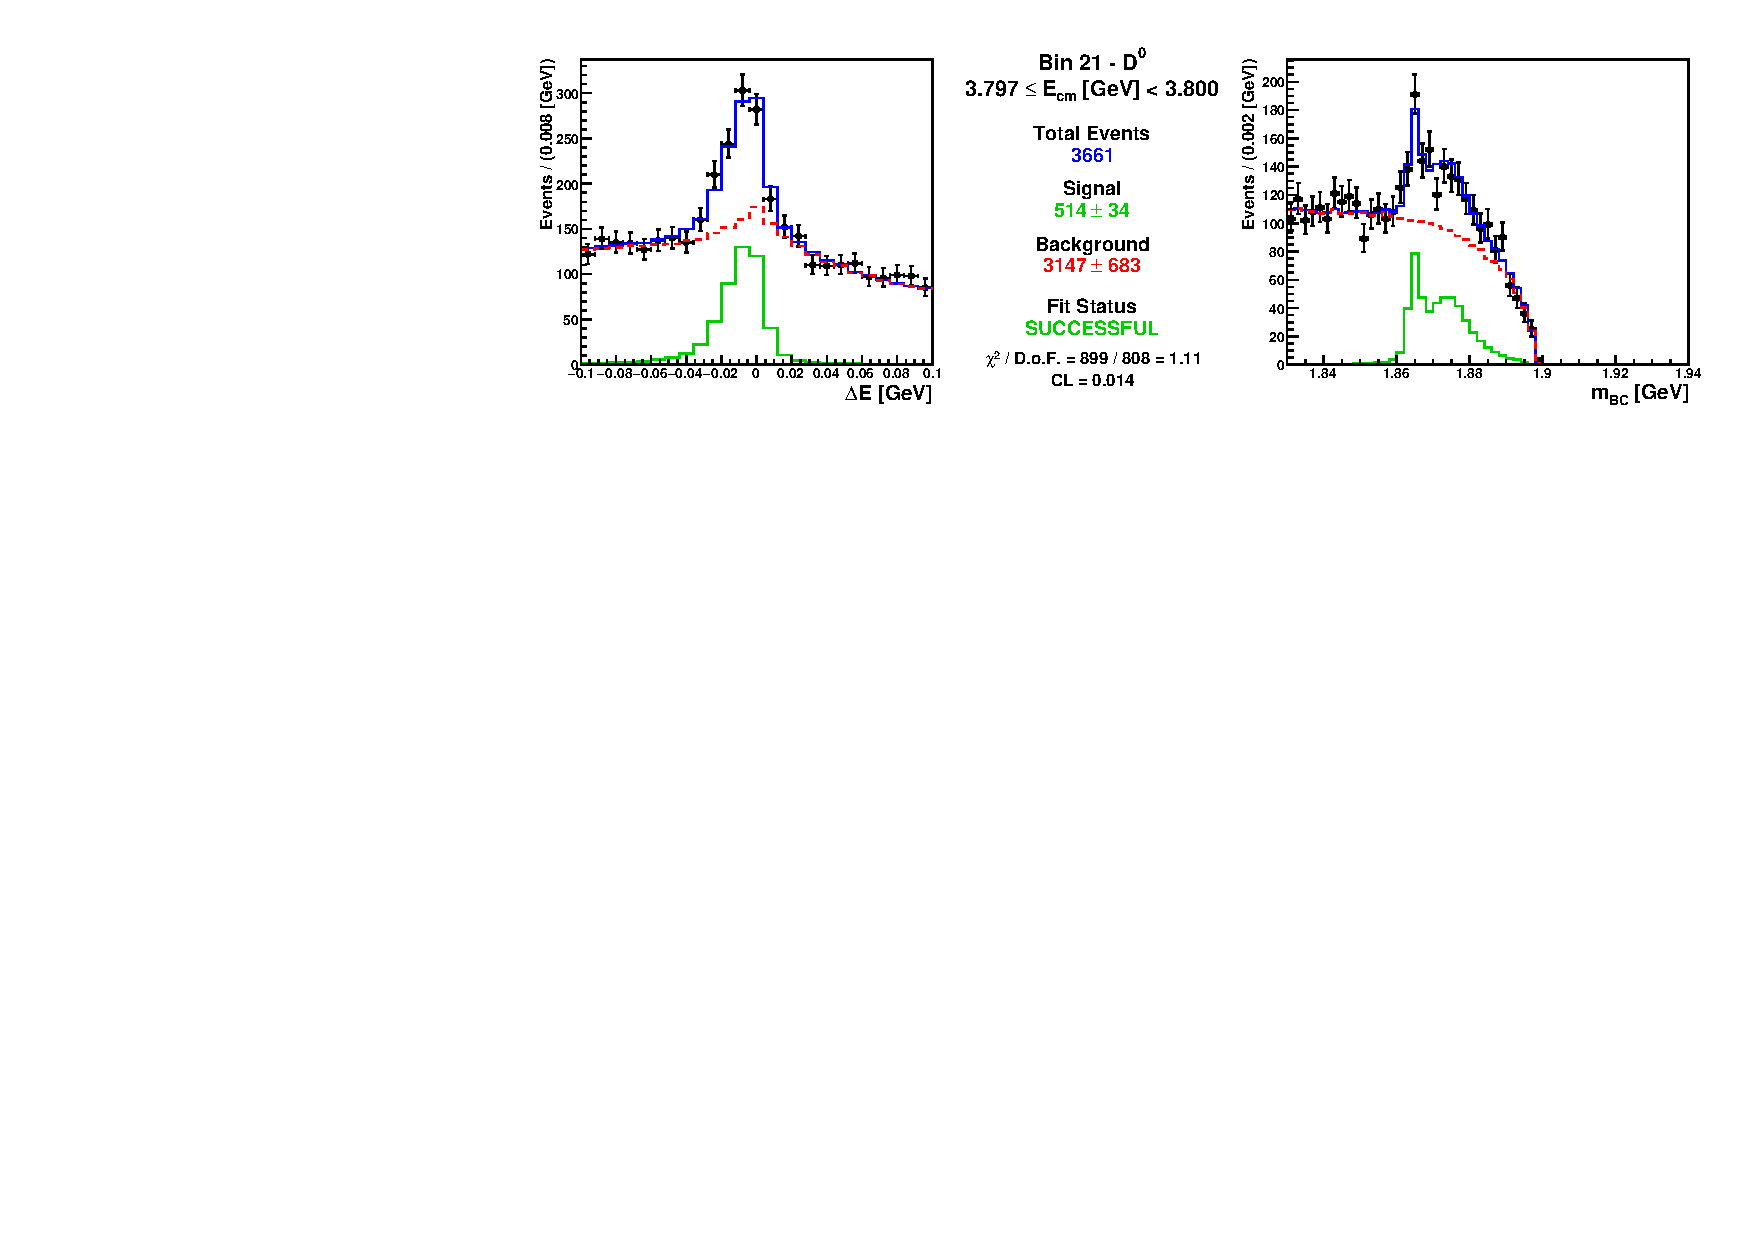
\includegraphics[trim={12cm 0 0 0},clip,width=0.3\linewidth]{../figures/plots/fit_results/D0_bin_21.pdf}
\end{figure}
\vspace{-0.5cm}
\begin{figure}
{\small \hspace{1cm} At Born Minimum \hspace{3cm} Above}
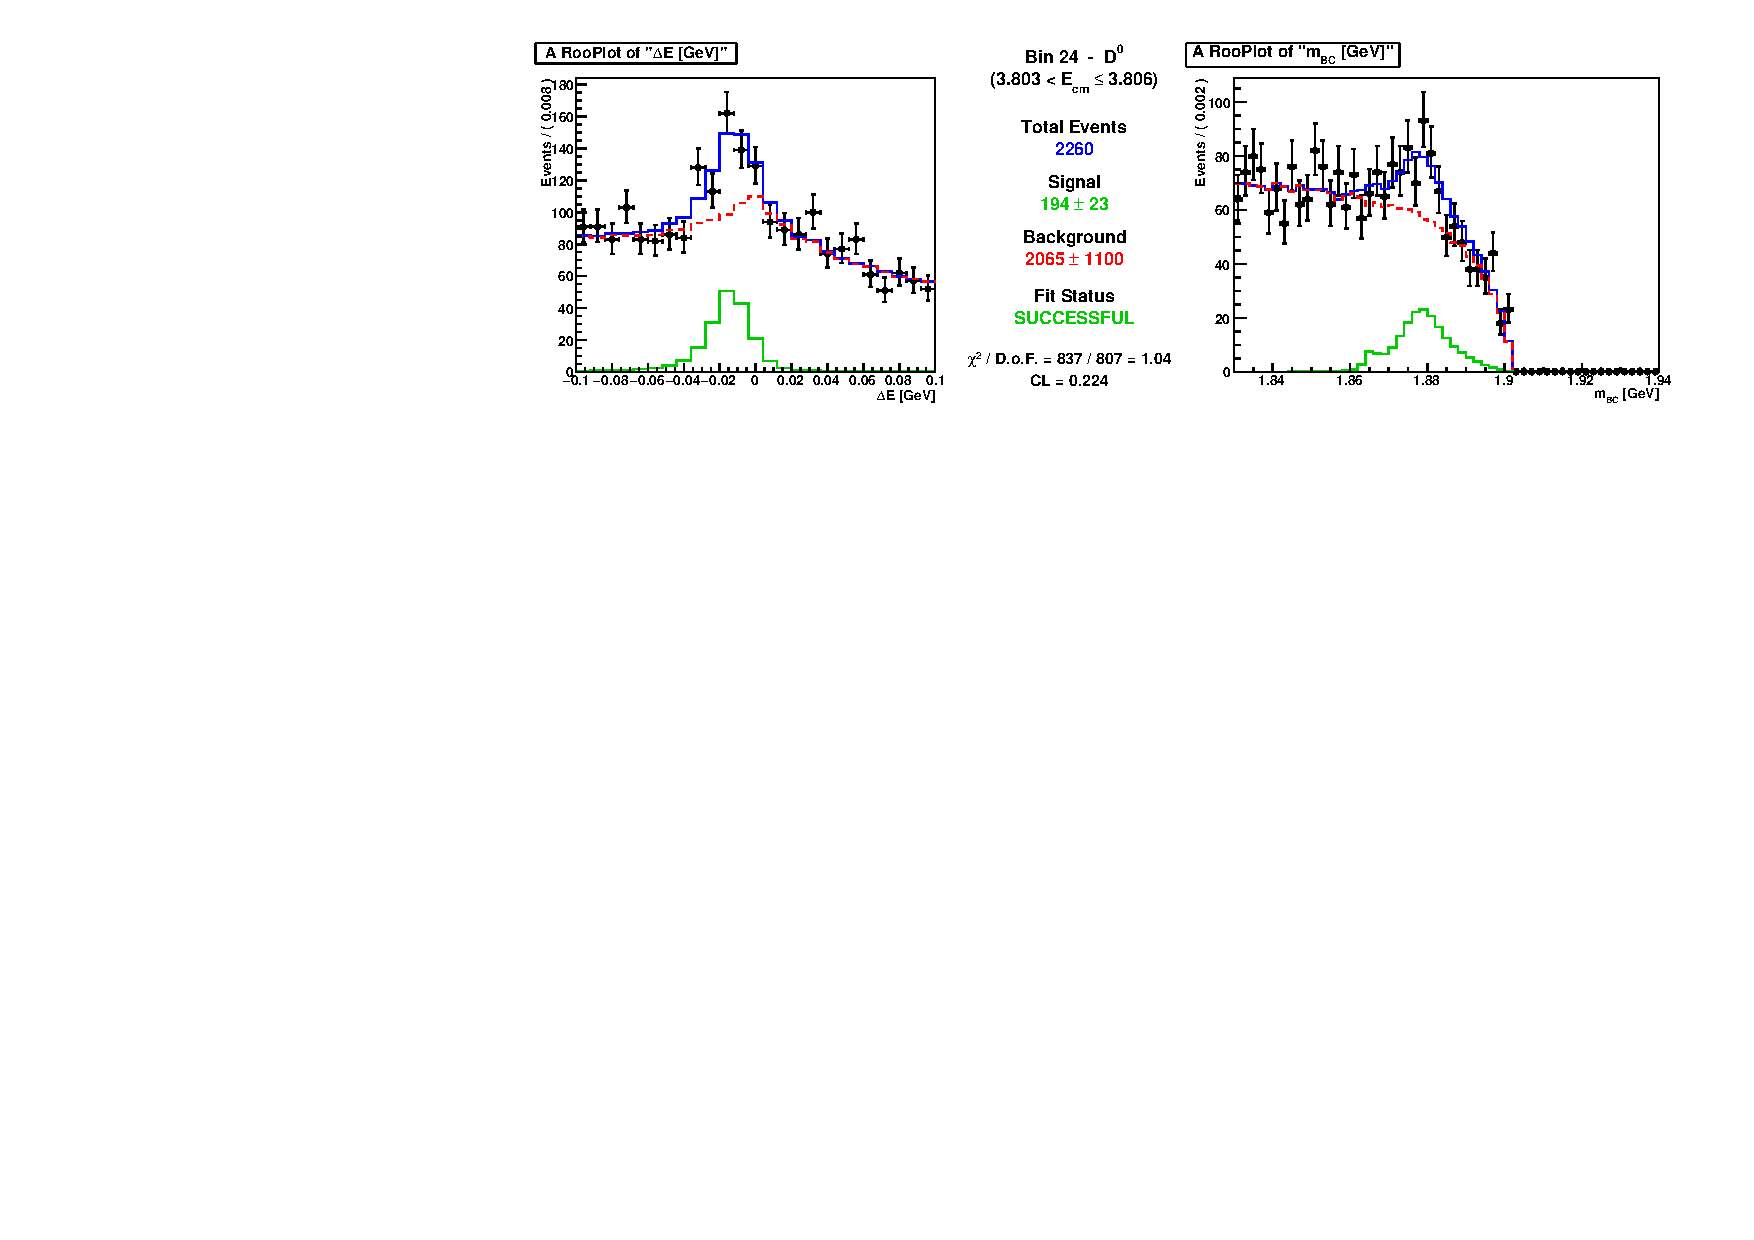
\includegraphics[trim={12cm 0 0 0},clip,width=0.3\linewidth]{../figures/plots/fit_results/D0_bin_24.pdf}
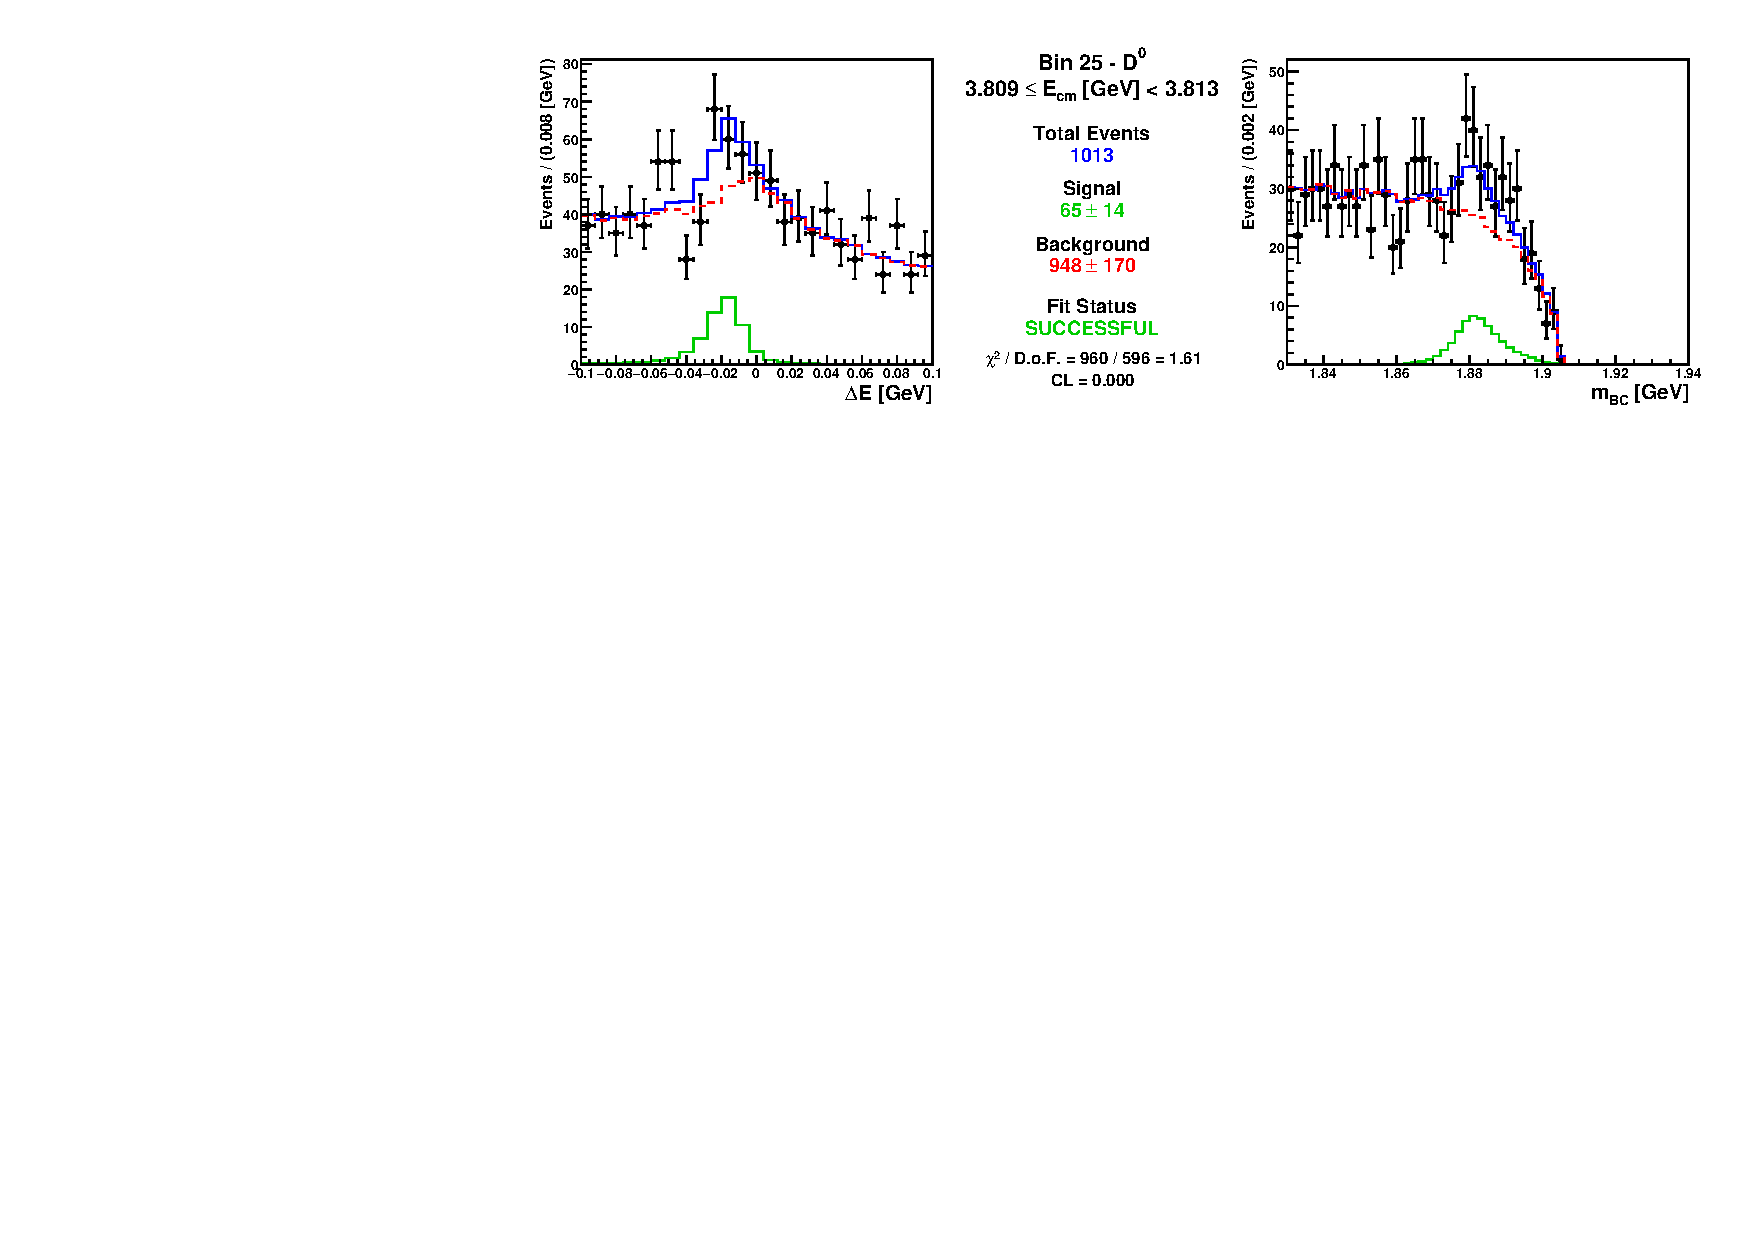
\includegraphics[trim={12cm 0 0 0},clip,width=0.3\linewidth]{../figures/plots/fit_results/D0_bin_25.pdf}
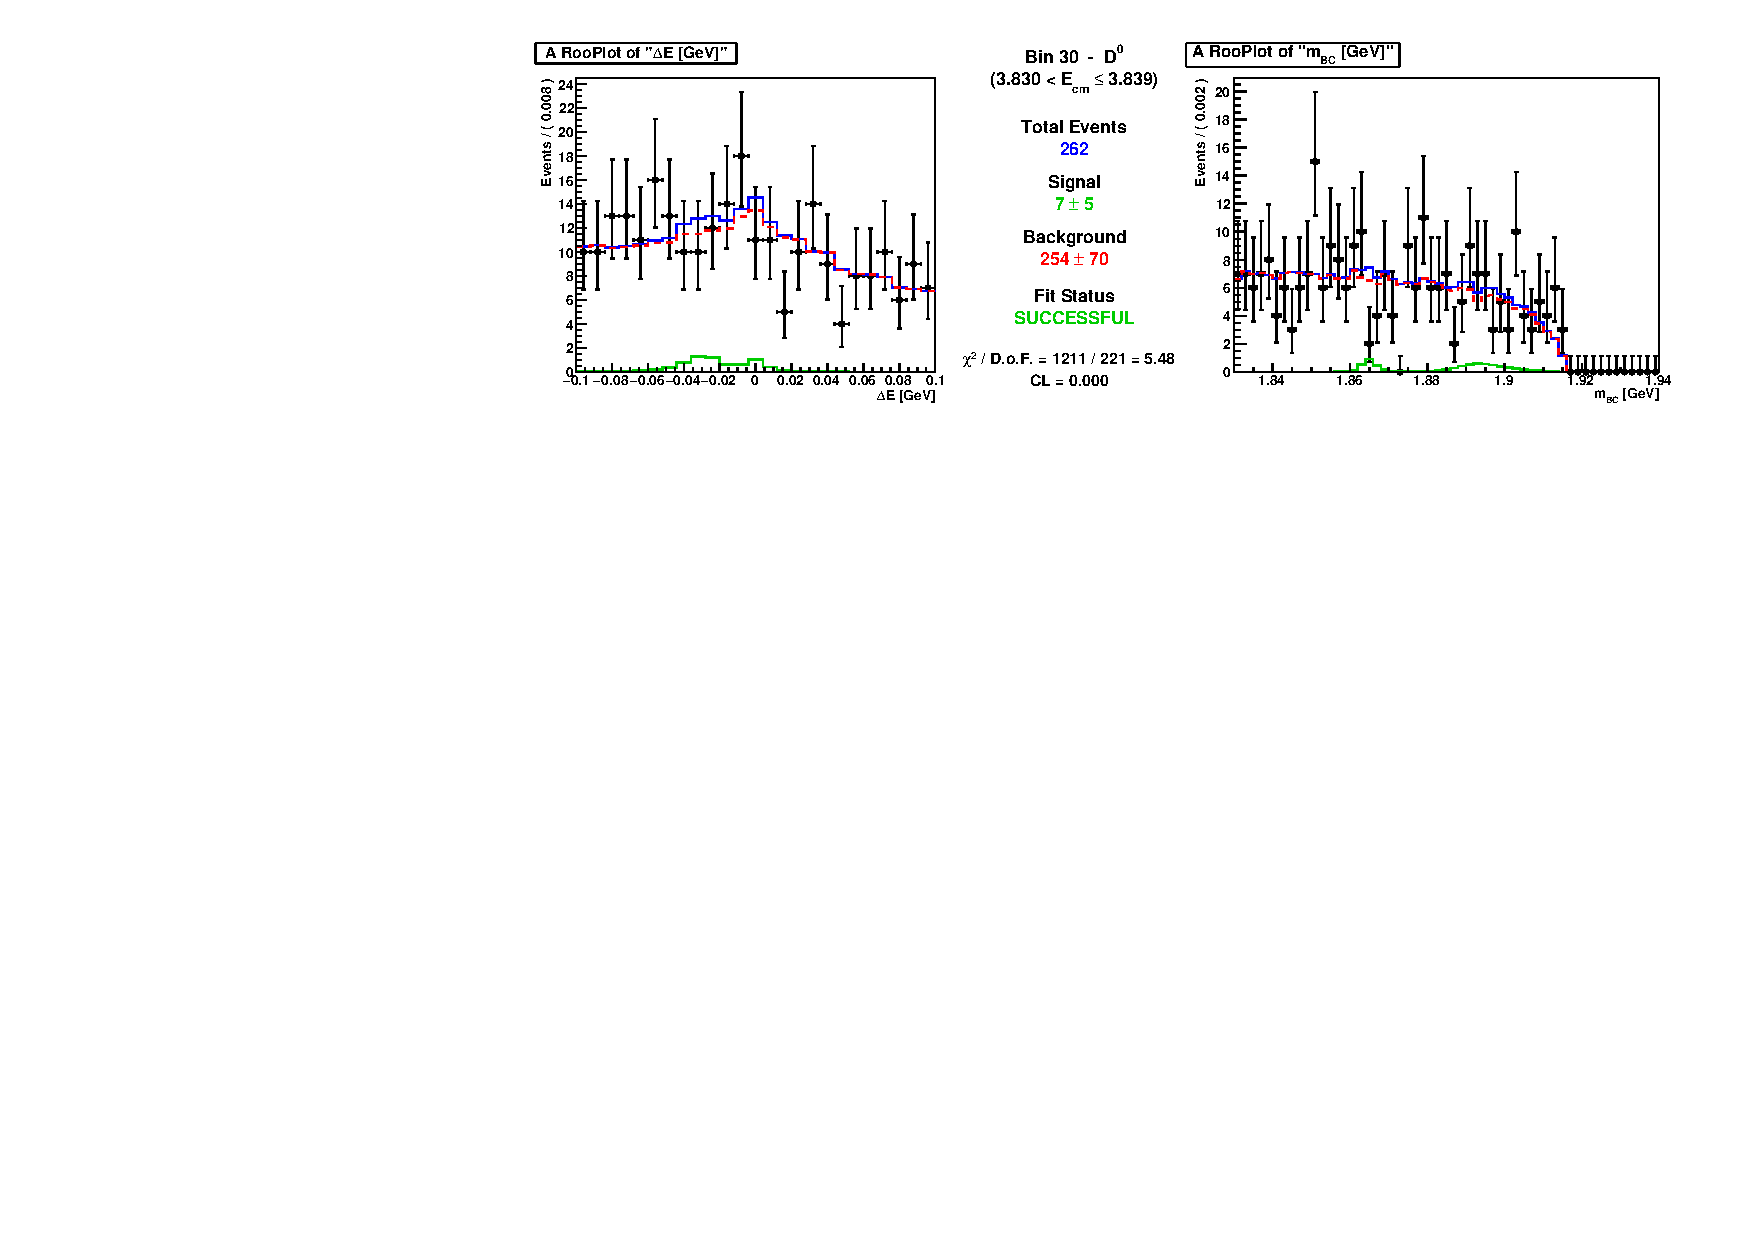
\includegraphics[trim={12cm 0 0 0},clip,width=0.3\linewidth]{../figures/plots/fit_results/D0_bin_30.pdf}
\end{figure}
}

\addframe{Coulomb Interaction}{
\additem{Significantly worse results when including value for ${\color{red} \zDD}$ ($\chi^2 \approx 5$)
\additem{Results shown previously use ${\color{red} \zDD} = 1$ for calculations}
}
\additem{Ratio of cross sections ($\sigma_{\Dp} / \sigma_{\DO}$) prefers excluding value
\additem{Unclear explanation for behavior, but consistent with $\Upsilon \rightarrow B\overline{B}$ studies}
}
\begin{figure}
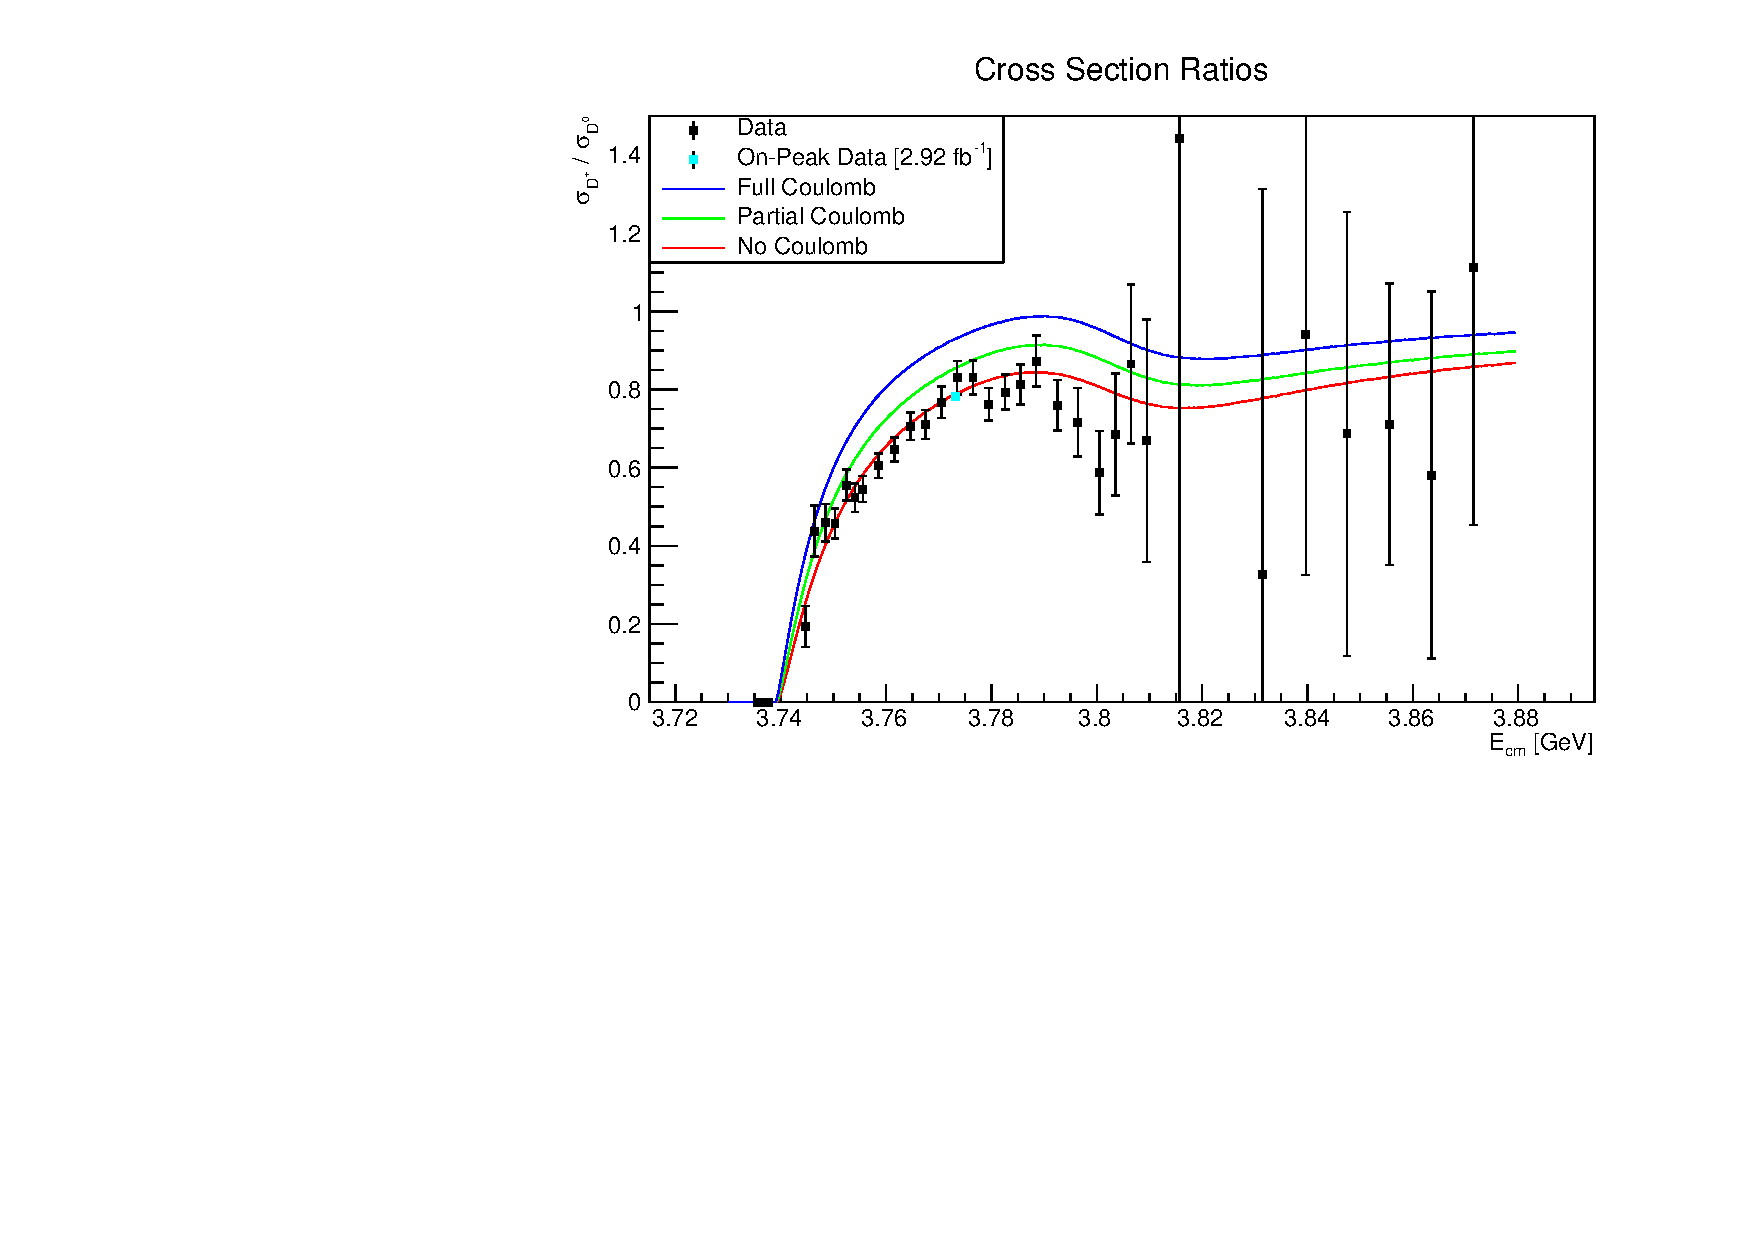
\includegraphics[scale=0.43]{../figures/plots/Coulomb_ratio.pdf}
\end{figure}
}

\addframe{Systematic Uncertainties}{
\additem{Examine uncertainty from parameters involved throughout procedure
\additem{Individually increase / decrease value by the uncertainty of each}
\additem{Re-fit cross section with altered values and take maximal variation}
}
\additem{Many uncertainties adjust overall scale of cross section normalization
\additem{Only affects the value of $\GeepsipptoDDbar$}
}

\begin{table}
\centering
\begin{tabular}{l|c|l}
\mccl{1}{Name} & Change & \mcc{1}{Description} \\
\hline
Luminosity              & $\lum$                     & \SI{1.0}{\%} \\
$\pipm / \Kpm$ Tracking & $\epsilon_{i \text{ rec}}$ & \SI{1.0}{\%} per $\pipm$ or $\Kpm$ in the mode \\
$\piO$ Tracking         & $\epsilon_{i \text{ rec}}$ & \SI{2.0}{\%} per $\piO$ in the mode \\
$\Ks$ Tracking          & $\epsilon_{i \text{ rec}}$ & \SI{1.5}{\%} per $\Ks$ in the mode \\
Single Tag Fits         & $N_D$                      & Adjust by fit difference (small) \\
PDG Branching Fractions & $\epsilon_{i \text{ rec}}$ & Adjust by PDG errors \\
\hline
\end{tabular}
\end{table}
}


\addframe{Systematic Uncertainties}{
\additem{\textbf{Meson Radii}
\additem{Adjust values of $R_{\psip}$ and $R_{\psipp}$ by \SI{25}{\%} (from KEDR)}
\additem{Take max variation over all four combinations of up / down on each}
\additem{Accounts for most significant source of systematic uncertainty}
}

\additem{\textbf{MC Iteration} (negligible)
\additem{Take difference in parameters before / after Born level modification}
}

\additem{\textbf{MC ISR Generation} (negligible)
\additem{Take difference in fit results with KKMC vs. ConExc generators}
}

\additem{\textbf{Intermediate Resonances} (negligible)
\additem{Examine effects of $\rho^0 \rightarrow \pip \pim$ in the mode $\DpmodeA$}
\additem{Take difference in $K\pi$ vs. $\pi\pi$ invariant mass splits using `On-Peak' data}
}
}

\addframe{Systematic Uncertainties}{
\additem{Uncertainties summed in quadrature (assumed independent)}
\additem{Total contribution similar to statistical error for most parameters
\additem{Value for $\Mpsipp$ is small, but has very small statistical error}
}

\begin{table}
\footnotesize
\centering
\renewcommand\arraystretch{1.0}
\begin{tabular}{c|cccc}
\hline 
Systematic & $\Mpsipp$ [\%] & $\Gpsipp$ [\%] & $\GeepsipptoDDbar$ [\%] & $\Ppsipp$ [\%] \\
\hline 
Luminosity              & 0.000 & 0.004 & 1.005 & 0.014 \\
$\Kpm / \pipm$ Tracking & 0.000 & 0.008 & 2.646 & 0.033 \\
$\piO$ Tracking         & 0.000 & 0.012 & 0.746 & 0.028 \\
$\Ks$ Tracking          & 0.000 & 0.004 & 0.260 & 0.019 \\ 
Single Tag Fits         & 0.000 & 0.012 & 0.213 & 0.008 \\
PDG Errors              & 0.000 & 0.017 & 2.840 & 0.036 \\
Meson Radii             & 0.016 & 2.411 & 3.512 & 1.477 \\
\hline
Total [\%]                      & 0.016 & 2.411 & 5.389 & 1.479 \\
Relative Stat. Error [$\sigma$] & 3.000 & 1.088 & 1.342 & 1.229 \\
\hline
\end{tabular} 
\end{table}
}


\addframe{Form Factor Uncertainty}{
\additem{Notable discrepancy between choices of non-resonant form factor
\additem{Both methods provide reasonably good fit with data}
\additem{Use difference of Exponential and VDM fit values as uncertainty}
\additem{Follow example of KEDR by treating as model-dependent uncertainty}
}

\begin{table}
\footnotesize
\centering
\renewcommand\arraystretch{1.0}
\begin{tabular}{c|cccc}
\hline 
Form Factor & $\Mpsipp$ [\si{\GeV}] & $\Gpsipp$ [\si{\MeV}] & $\GeepsipptoDDbar$ [\si{\eV}] & $\Ppsipp$ [\si{\degree}] \\
\hline 
Exponential & 3.7821 & 26.004 & 233.13 & 214.60 \\
VDM         & 3.7808 & 24.098 & 215.83 & 207.12 \\
\hline
Difference & 0.0013 & \pp1.906 & \pp17.30 & \PP7.48 \\
\hline
\end{tabular} 
\end{table}
}

\addframe{Final Results}{
\additem{Results limited by systematics and model-dependency
\begin{table}
\centering
\renewcommand\arraystretch{1.0}
\begin{tabular}{C{2.25cm} l c}
\hline 
$\Mpsipp$          & $    3780.8 \pm     0.2   \pm    0.6   \pm   1.3$ & $[\si{\MeV}]$   \\
$\Gpsipp$          & $\PP 24.1   \pm     0.5   \pm    0.6   \pm   1.9$ & $[\si{\MeV}]$   \\
$\GeepsipptoDDbar$ & $\PP 216 \; \pm \pp  9 \; \pm    11 \; \pm    17$ & $[\si{\eV}]$    \\
$\Ppsipp$          & $\PP 207 \; \pm \pp  3 \; \pm \pp 3 \; \pm \pp 7$ & $[\si{^\circ}]$ \\
\hline
\multicolumn{3}{l}{\footnotesize Errors are statistical, systematic, and model-dependent, respectively}
\end{tabular} 
\end{table}
}

\additem{Results consistent with KEDR and very inconsistent with PDG
\begin{table}
\footnotesize
\centering
\renewcommand\arraystretch{1.0}
\begin{tabular}{c L{2.8cm} L{2.5cm} L{2.5cm}}
\hline
Method & $\Mpsipp$ [MeV] & $\Gpsipp$ [MeV] & $\GeepsipptoDDbar$ [eV] \\
\hline
Exponential & $3782.1 \pm 0.3 \pm 0.6$ & $26.0 \pm 0.6 \pm 0.7$ & $233 \pm 10 \pm 13$ \\
VDM         & $3780.8 \pm 0.2 \pm 0.6$ & $24.1 \pm 0.6 \pm 0.6$ & $216 \pm  9 \pm 12$ \\
KEDR        & $3779.2^{+1.8 +0.5 +0.3}_{-1.7 -0.7 -0.3}$ & $24.9^{+4.6 + 0.5 +0.2}_{-4.0 -0.6 -0.9}$ & $154^{+79 +17 +13}_{-58 -9\pp -25}$, $414^{+72 +24 +90}_{-80 -26 -10}$ \\
PDG         & $3773.15 \pm 0.33$     & $27.2 \pm 0.9$       & $[262 \pm 18] \times ~\BDD$ \\
\hline
\end{tabular}
\end{table}
}
}


\sectionframe{Measurement of the $\NonDDbar$ Branching Fraction}
% Show images of data counts, extrapolations, $\DDbar$ corrections

\addframe{Procedure}{
Event Selection

Hadron Cut Methods

Signal Counting Fits

MC Background Subtraction

Efficiency Extrapolation

$\DDbar$ Multiplicity Correction

Examination of Results for $\psipp$ Data

Background Investigation

Examination of Results for Scan Data

}

\addframe{Data Samples}{
\additem{Use data from continuum (Old / New), $\psipp$ (R1 / R2), and scan}

\begin{columns}

\column{.4\textwidth} % Left column and width
\vspace{0.8cm}
\additem{$\Ecm$ measured as before
\additem{4-6 \si{\MeV} shift in new continuum samples}
\additem{No shift for old continuum samples}
}

\column{.6\textwidth} % Right column and width
\begin{table}
\footnotesize
\centering
\renewcommand\arraystretch{1.0}
\begin{tabular}{l|c r}
\hline
Sample Name & $\Ecm$ [\si{\GeV}] & Luminosity [\si{\invpb}] \\
\hline
3500 (New)    & 3.496 & \num{  3.680 \pm 0.009} \\
3542 (New)    & 3.538 & \num{  3.481 \pm 0.009} \\
3600 (New)    & 3.596 & \num{  0.395 \pm 0.019} \\
3650 (New)    & 3.644 & \num{  5.420 \pm 0.009} \\
3671 (New)    & 3.665 & \num{  4.669 \pm 0.009} \\
3650 (Old)    & 3.650 & \num{ 44.334 \pm 0.009} \\
$\psipp$ (R1) & 3.773 & \num{926.922 \pm 0.092} \\
$\psipp$ (R2) & 3.773 & \num{1978.92 \pm 0.091} \\
\hline
\end{tabular}
\end{table}

\end{columns}

\additem{Requires precise $\Ecm$ measurement for extrapolation procedure
\additem{Cross section of $\psip$ rapidly changes near its peak}
}
}

\addframe{Event Selection Criteria}{
\additem{Apply cuts on charged (neutral) tracks in the MDC (EMC)}
\additem{Apply cuts on highest energy / momentum to remove $\ee \rightarrow \{\ee, \; \yy\}$ backgrounds}

\additem{Apply groups of cuts to select multihadron events
\additem{Number of Tracks}
\additem{Visible Energy}
\additem{Visible Momentum ($z$-direction)}
\additem{Max Shower Energy}
\additem{Total Shower Energy}
}
\additem{Values for group cuts dependent on level of impact
\additem{Standard (SHAD), Loose (LHAD), Tight (THAD)}
}
}

\addframe{Signal Counting}{
\additem{Identify events using average distance of closest approach in $z$ ($V_z$)
\additem{Signal tracks will originate within few \si{\cm} of vertex}

\additem{Background tracks can originate away from collision point}
}
\additem{Fit with a double Gaussian (sig) + $2^{\text{nd}}$-order polynomial (bkg) shape}

\begin{figure}
\centering
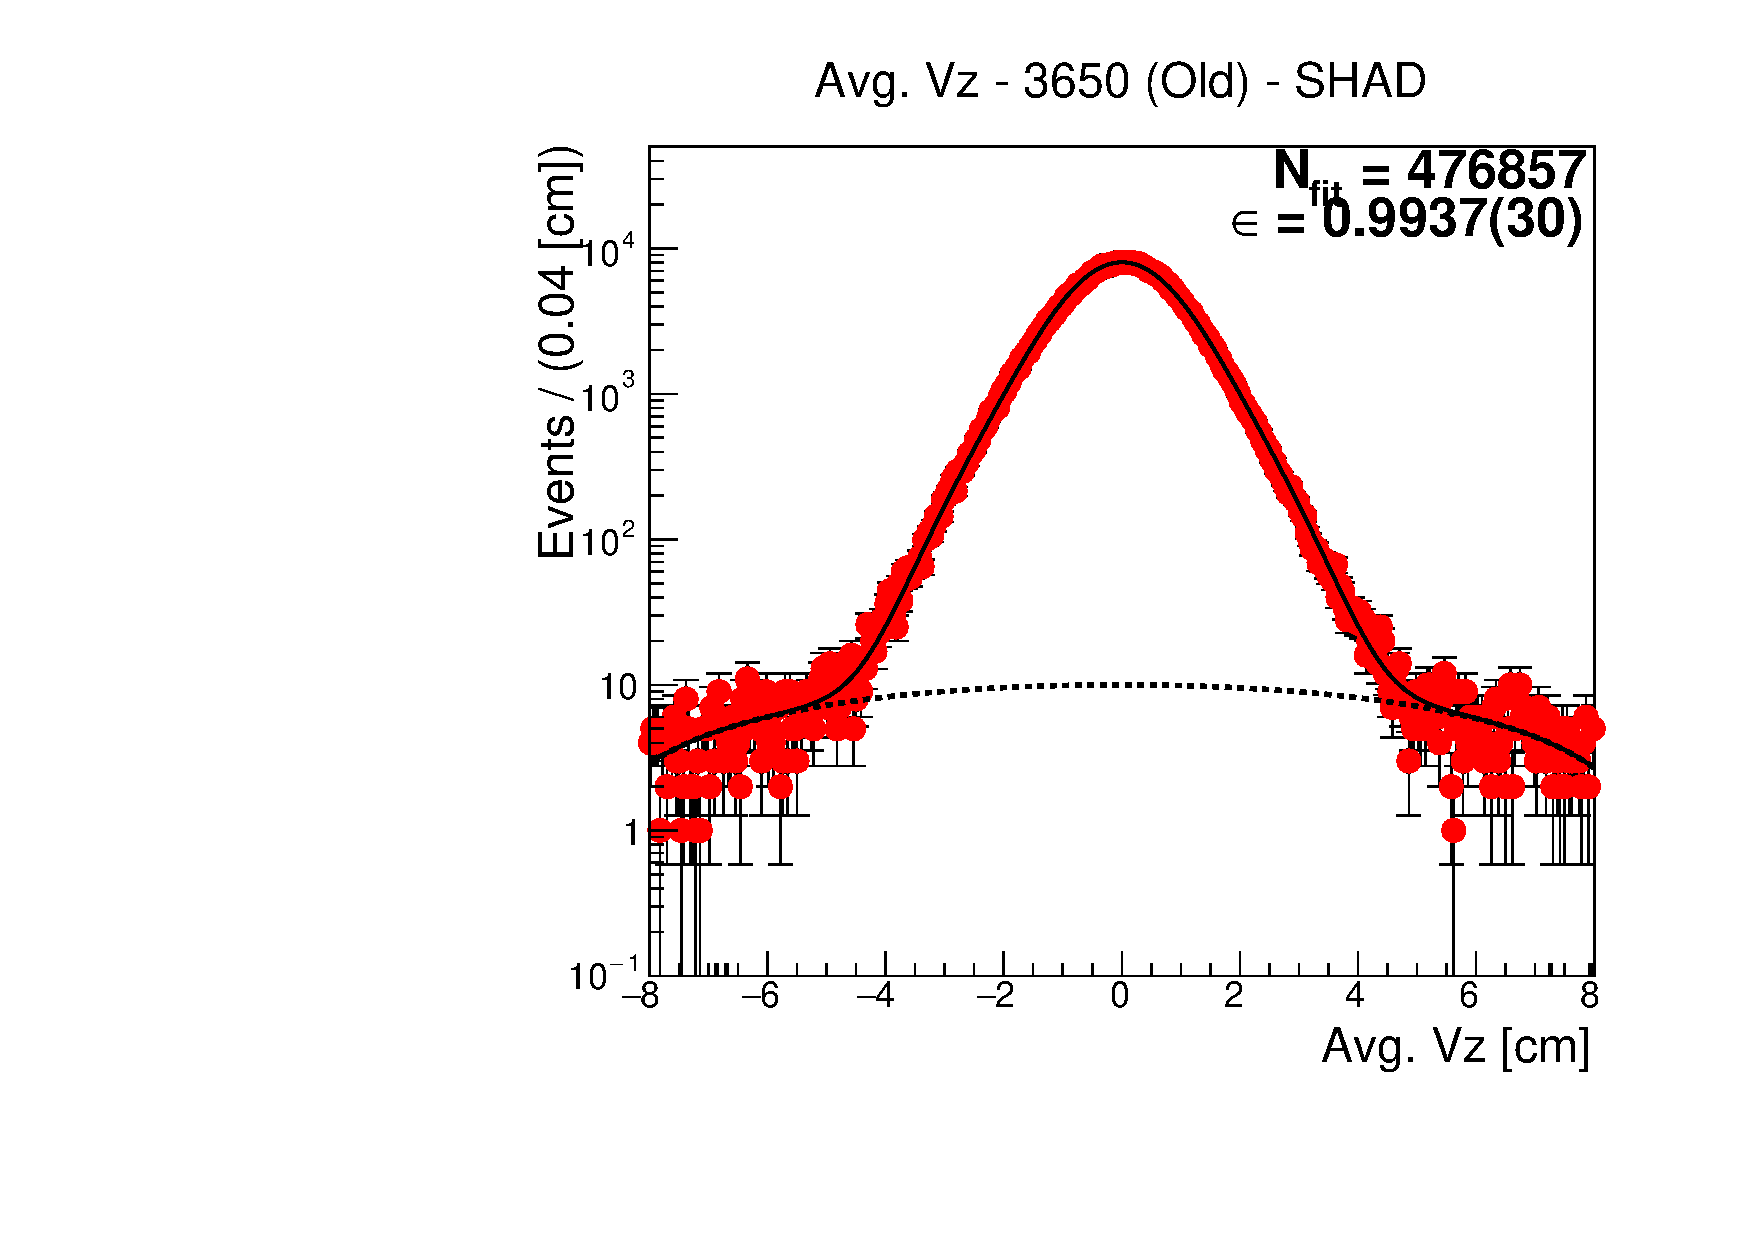
\includegraphics[width=0.33\textwidth]{../figures/plots/nonDDbar_fit_results/3650_old/fit_old_3650_data_SHAD.pdf}
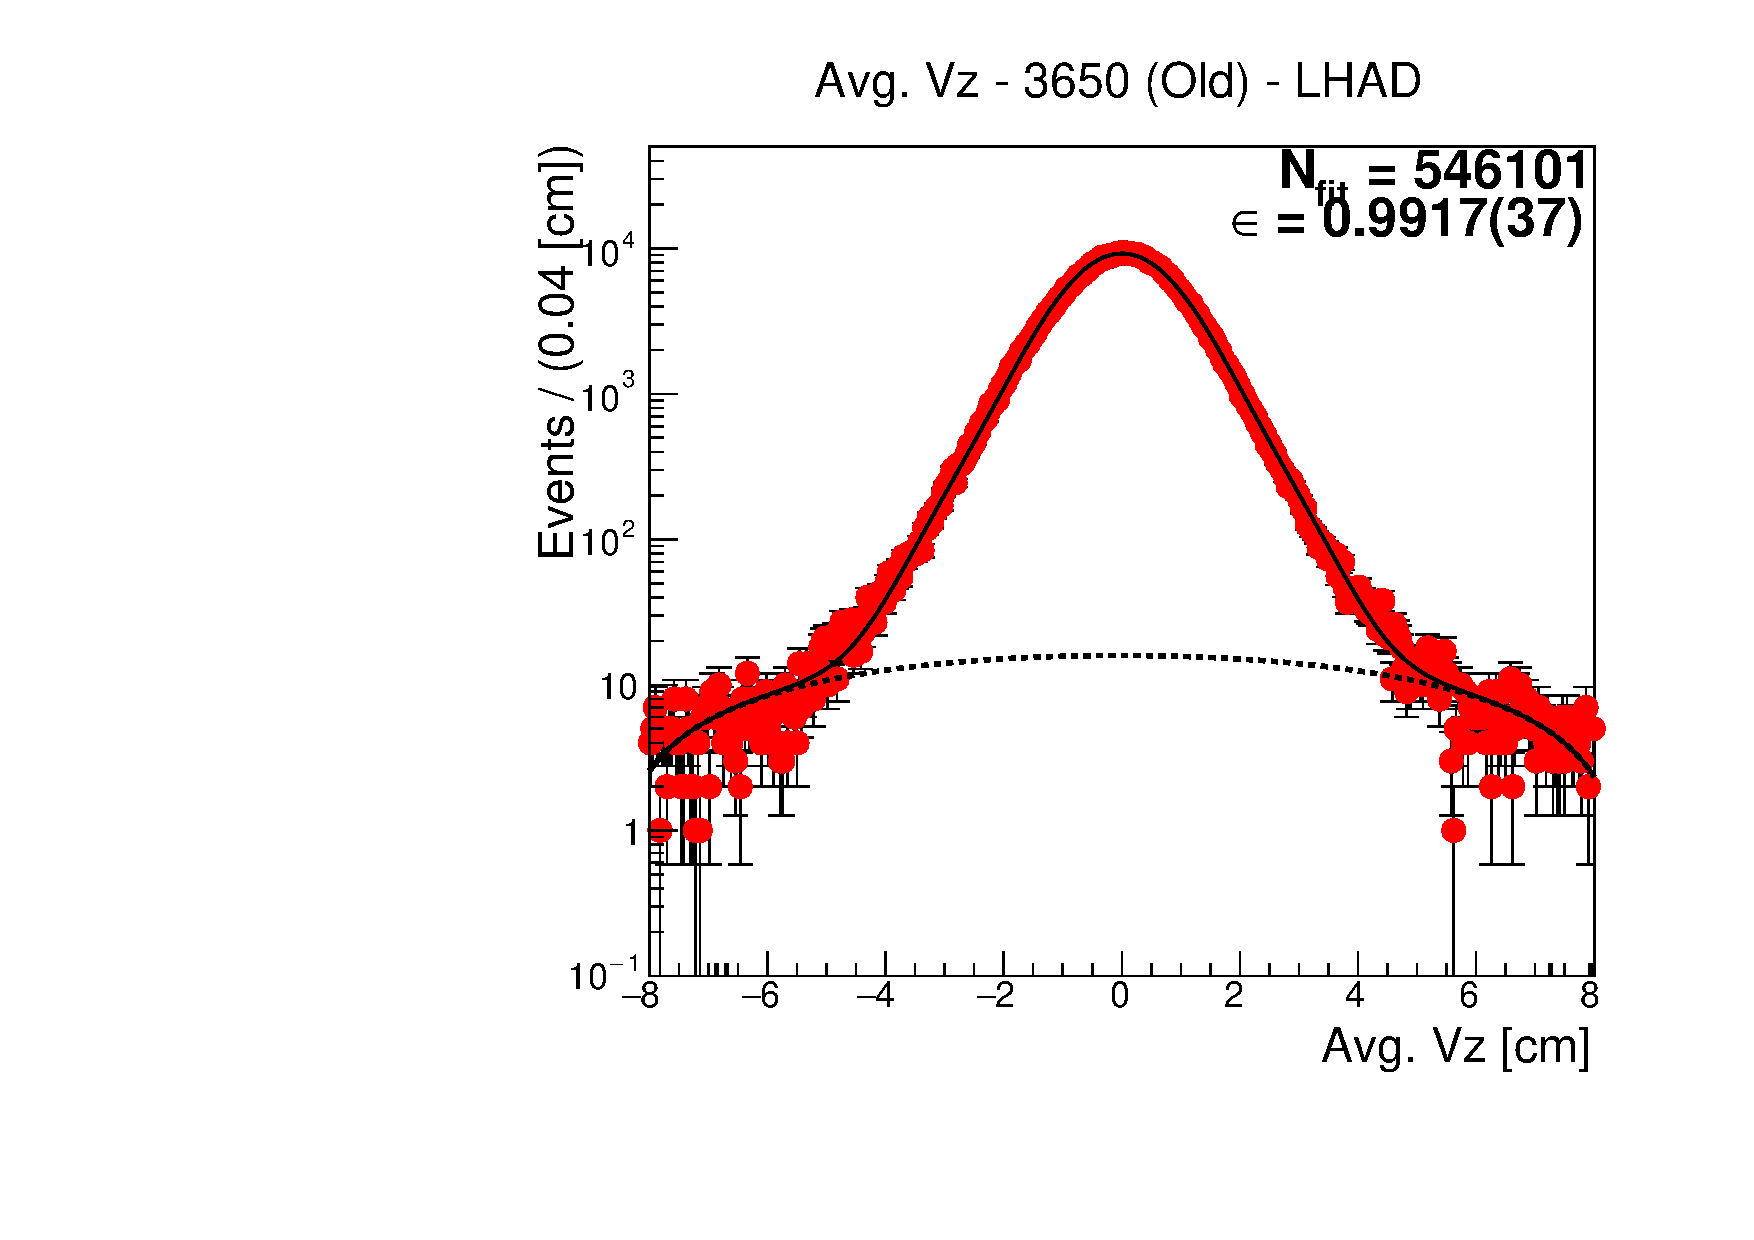
\includegraphics[width=0.33\textwidth]{../figures/plots/nonDDbar_fit_results/3650_old/fit_old_3650_data_LHAD.pdf}
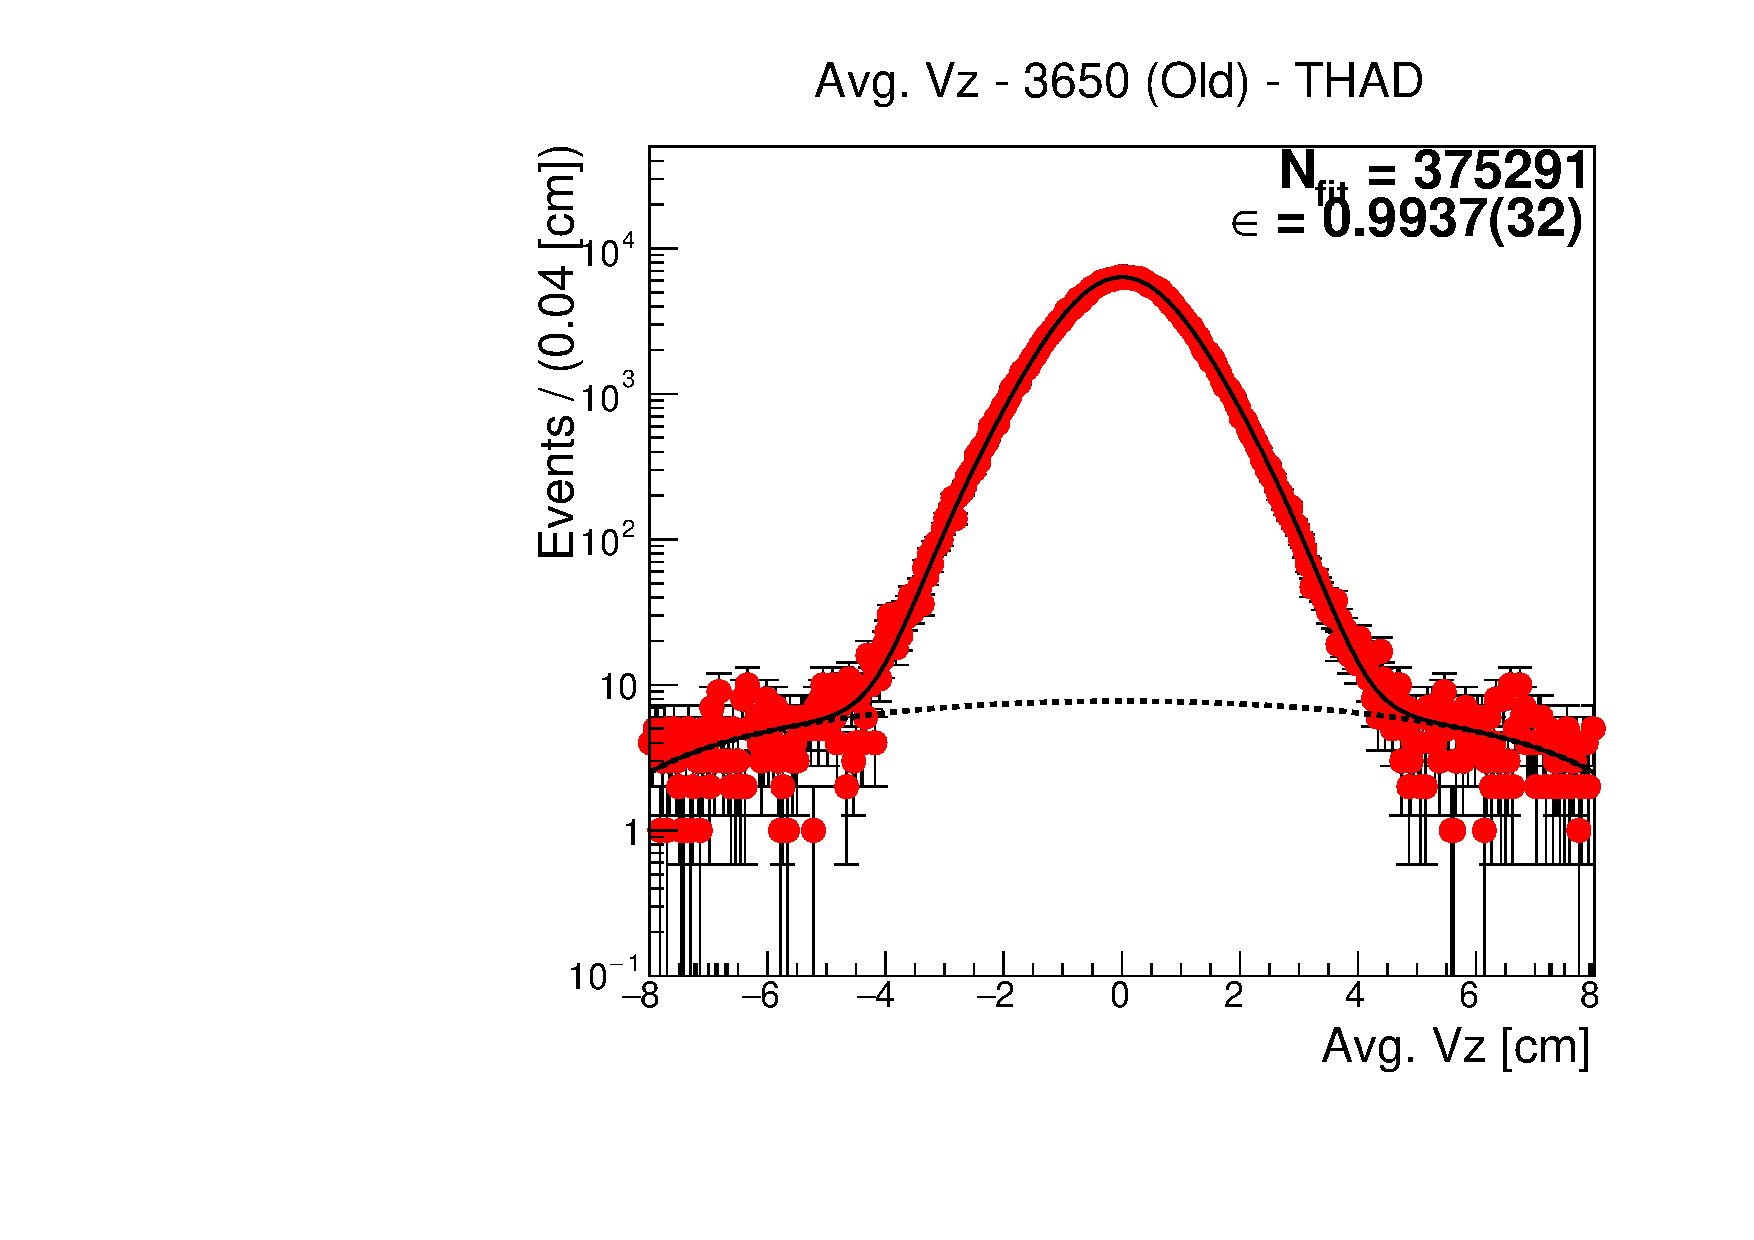
\includegraphics[width=0.33\textwidth]{../figures/plots/nonDDbar_fit_results/3650_old/fit_old_3650_data_THAD.pdf}
\end{figure}

}

\addframe{Background Subtraction}{
\additem{Need to determine background contributions seen in data
\addcenter{$\Nhad = \lum \times \sigma \times \effmc = \lum \times \sigma \times \left( \frac{ N_{\text{rec}} }{ N_{\text{gen}} } \right)$}
}

\begin{table}
\footnotesize
\centering
\renewcommand\arraystretch{1.0}
\begin{tabular}{c|r|r@{$\; \pm \;$}r r@{$\; \pm \;$}r r@{$\; \pm \;$}r}
\hline
\multicolumn{8}{c}{3650 (Old) Reconstruction} \\
\hline
Sample & $\sigma$ [\si{\nb}] & \multicolumn{2}{c}{$\effmc$ (SHAD) [\%]} & \multicolumn{2}{c}{$\effmc$ (LHAD) [\%]} & \multicolumn{2}{c}{$\effmc$ (THAD) [\%]} \\
\hline
$\ee$           & 554.562 &  0.0006 & 0.0002 &  0.0008 & 0.0002 &  0.0001 & 0.0001 \\
$\mumu$         &   5.560 &  0.0033 & 0.0004 &  0.0044 & 0.0005 &  0.0029 & 0.0004 \\
$\tautau$       &   1.844 & 12.8351 & 0.0255 & 28.7692 & 0.0382 &  9.9371 & 0.0224 \\
$\yjpsi$        &   1.260 & 45.9222 & 0.0482 & 55.1722 & 0.0529 & 34.1250 & 0.0416 \\
$\yy$           &  21.530 &  0.0009 & 0.0002 &  0.0010 & 0.0002 &  0.0005 & 0.0002 \\
$\twophoton$    &   1.257 &  2.4109 & 0.0110 &  4.6297 & 0.0153 &  1.6468 & 0.0091 \\
$\psip^\dagger$ &   0.150 & 62.9891 & 0.0078 & 69.2882 & 0.0082 & 51.6942 & 0.0071 \\
\hline
\mcc{8}{$^\dagger$Contribution from $\psip$ assumes standard Breit-Wigner shape}
\end{tabular}
\end{table}

}

\addframe{Background Subtraction}{

\additem{Subtract backgrounds from total data events to get signal hadrons
\additem{Ignore negligible samples for extrapolation \{$\ee, \; \mumu, \; \yy$\}}
}

\begin{table}
\footnotesize
\centering
\renewcommand\arraystretch{1.0}
\begin{tabular}{c|r@{$\; \pm \;$}r r@{$\; \pm \;$}r r@{$\; \pm \;$}r}
\hline
\multicolumn{7}{c}{3650 (Old) Results} \\
\hline
Sample         & \multicolumn{2}{c}{$\Nhad$ (SHAD)} & \multicolumn{2}{c}{$\Nhad$ (LHAD)} & \multicolumn{2}{c}{$\Nhad$ (THAD)} \\
\hline
Data            & 477001 & 691 & 546546 & 739 & 375380 & 613 \\
$\ee{^*}$       &    149 &  43 &    187 &  48 &     12 &  12 \\
$\mumu{^*}$     &      8 &   1 &     11 &   1 &      7 &   1 \\
$\tautau$       &  10490 &  30 &  23514 &  59 &   8122 &  25 \\
$\yjpsi$        &  25658 &  60 &  30826 &  71 &  19067 &  46 \\
$\yy{^*}$       &      9 &   2 &     10 &   2 &      4 &   1 \\
$\twophoton$    &   1443 &   7 &   2771 &  11 &    986 &   6 \\
$\psip^\dagger$ &   4175 &   9 &   4593 &  10 &   3427 &   7 \\
\hline                                                       
Hadrons         & 435234 & 694 & 484842 & 745 & 343779 & 615 \\
\hline
\mcc{7}{$^\dagger$Contribution from $\psip$ assumes standard Breit-Wigner shape}
\end{tabular}
\end{table}

}

\addframe{Efficiency Extrapolation}{
\additem{Contribution of $\qqbar$ events above $\DDbar$ threshold not well modeled
\additem{Repeat procedure for new continuum data to extrapolate}
}
\addcenter{$\frac{ \epsilon(\Ecm) }{ \epsilon(3650) } = \left[ \frac{ \Nhad(\Ecm) }{ \Nhad(3650) } \right] \left[ \frac{ \lum(3650) }{ \lum(\Ecm) } \right] \bigg[ \frac{ \Ecm }{ 3650 } \bigg]^2$}
\begin{figure}
\centering
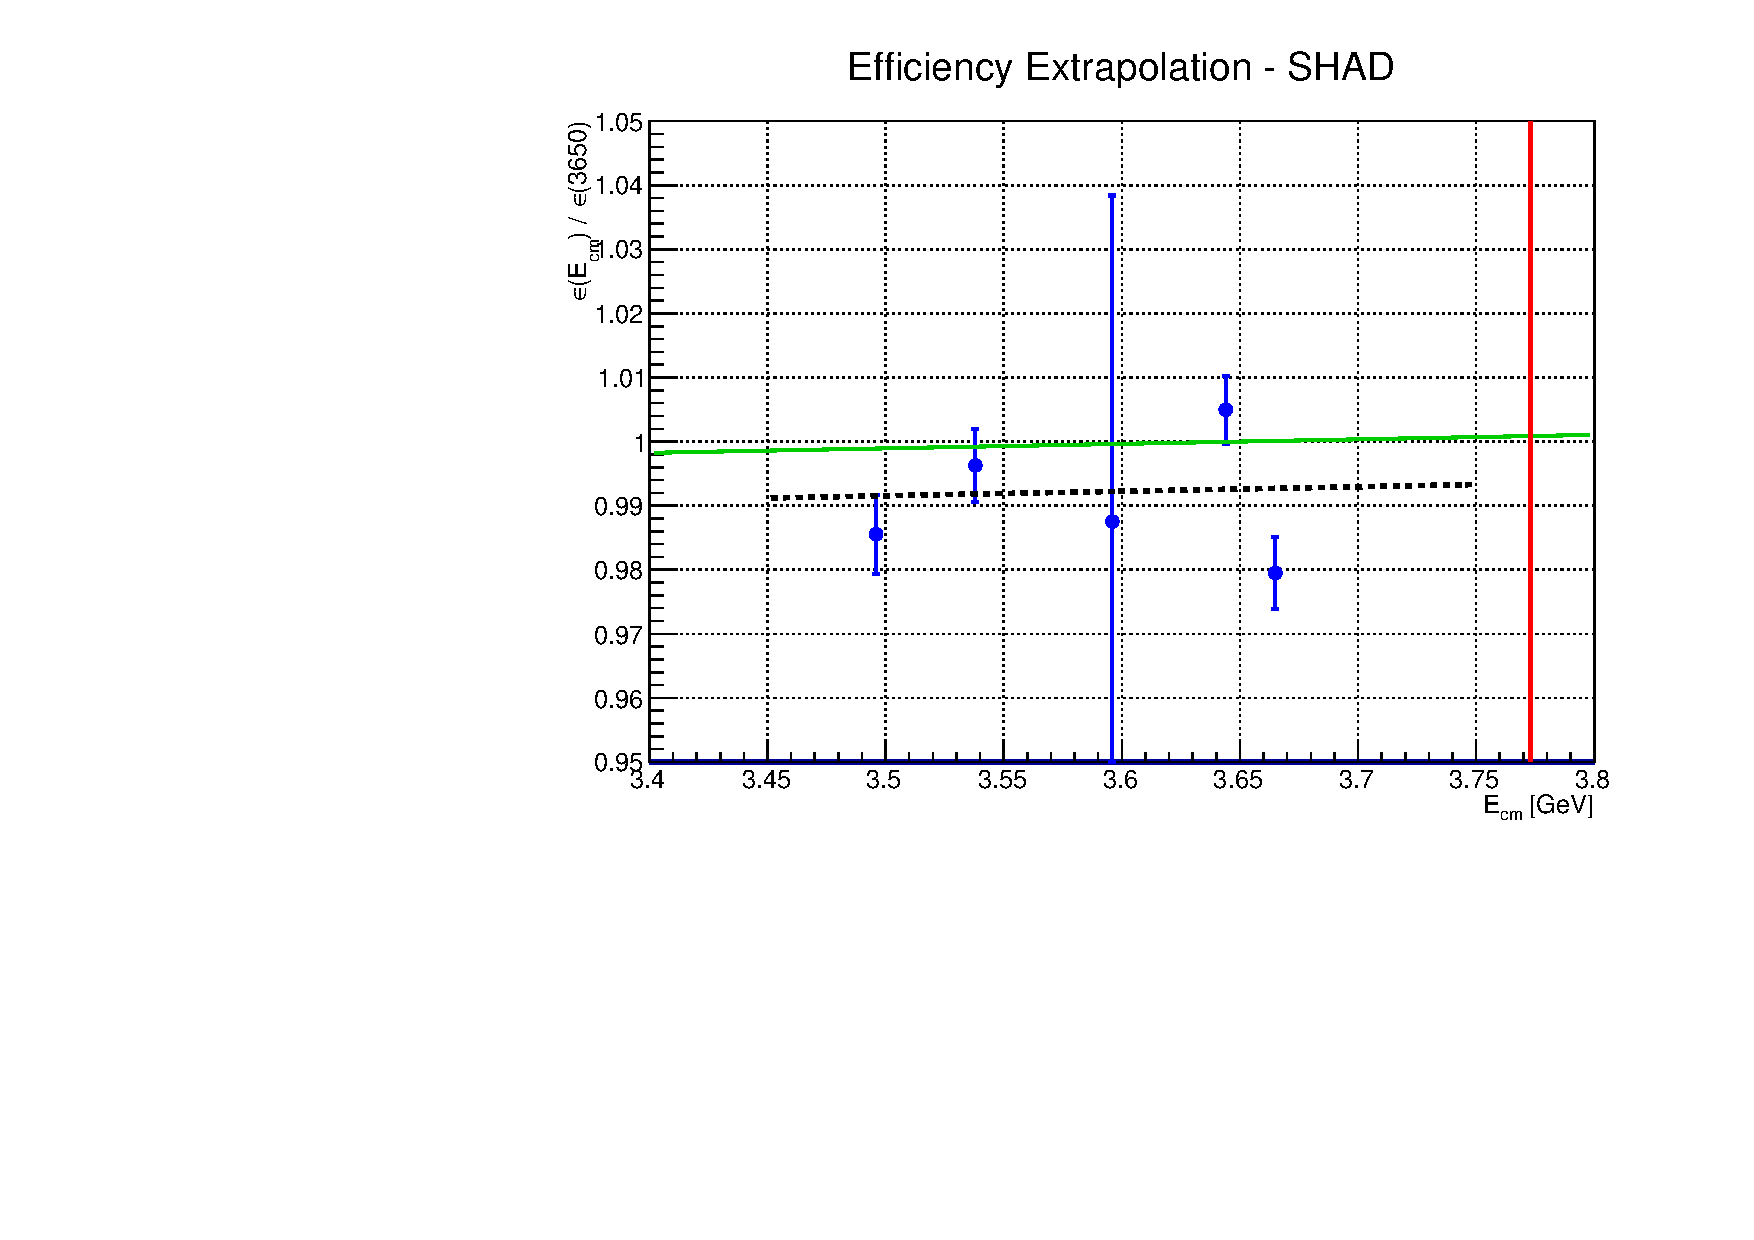
\includegraphics[width=0.6\textwidth]{../figures/plots/SHAD_psip_BW.pdf}
\end{figure}
}

\addframe{Procedure for $\psipp$ Data}{
\additem{Repeat procedure for $\psipp$ data samples
\additem{Use extrapolation to determine $\qqbar$ background contribution}
}
\additem{Modify included backgrounds to account for $\DDbar$ threshold
\additem{Use measurement of $\psipptoDDbar$ cross section for $\DDbar$ component
\additem{Use measurement from `On-Peak` sample for initial exploration}
}
\additem{Switch direct contribution from $\psip$ to radiative decays ($\ypsip$)
\additem{Use measurements from CLEO-c and BESIII for cross section value}
}
\additem{Neglect $\twophoton$ events due to minimal contribution in this region}
}
\additem{Need data-driven procedure to correctly determine $\DDbar$ efficiencies
\additem{MC samples unreliable at modeling track multiplicities}
\additem{Re-weight MC samples based off differences seen in data
\additem{Scale by track multiplicity ratios for data / MC}
}
}
}

\addframe{$\DDbar$ Efficiency Correction}{

\begin{columns}
\column{0.3\textwidth}
\vspace{-0.5cm}
\begin{table}
\footnotesize
\centering
\renewcommand\arraystretch{1.0}
\begin{tabular}{c|c}
\hline
Group & Multiplicity \\
\hline
SHAD & $\Ntrk > 2$ \\
LHAD & $\Ntrk > 1$ \\
THAD & $\Ntrk > 3$ \\
\hline
\end{tabular}
\end{table}

\begin{table}
\footnotesize
\centering
\renewcommand\arraystretch{1.0}
\begin{tabular}{c|c}
\hline
\mcc{2}{$\psipp$ R1 - $\DO$} \\
\hline 
Group & $(\effdata / \effmc)$ \\
\hline
SHAD & 0.9751 \\
LHAD & 0.9930 \\
THAD & 0.9662 \\
\hline
\end{tabular}
\end{table}

\vspace{-0.5cm}

\begin{table}
\footnotesize
\centering
\renewcommand\arraystretch{1.0}
\begin{tabular}{c|c}
\hline
\mcc{2}{$\psipp$ R1 - $\Dp$} \\
\hline 
Group & $(\effdata / \effmc)$ \\
\hline
SHAD & 0.9992 \\
LHAD & 1.0018 \\
THAD & 1.0064 \\
\hline
\end{tabular}
\end{table}



\column{0.7\textwidth}
\vspace{-0.6cm}
\begin{figure}
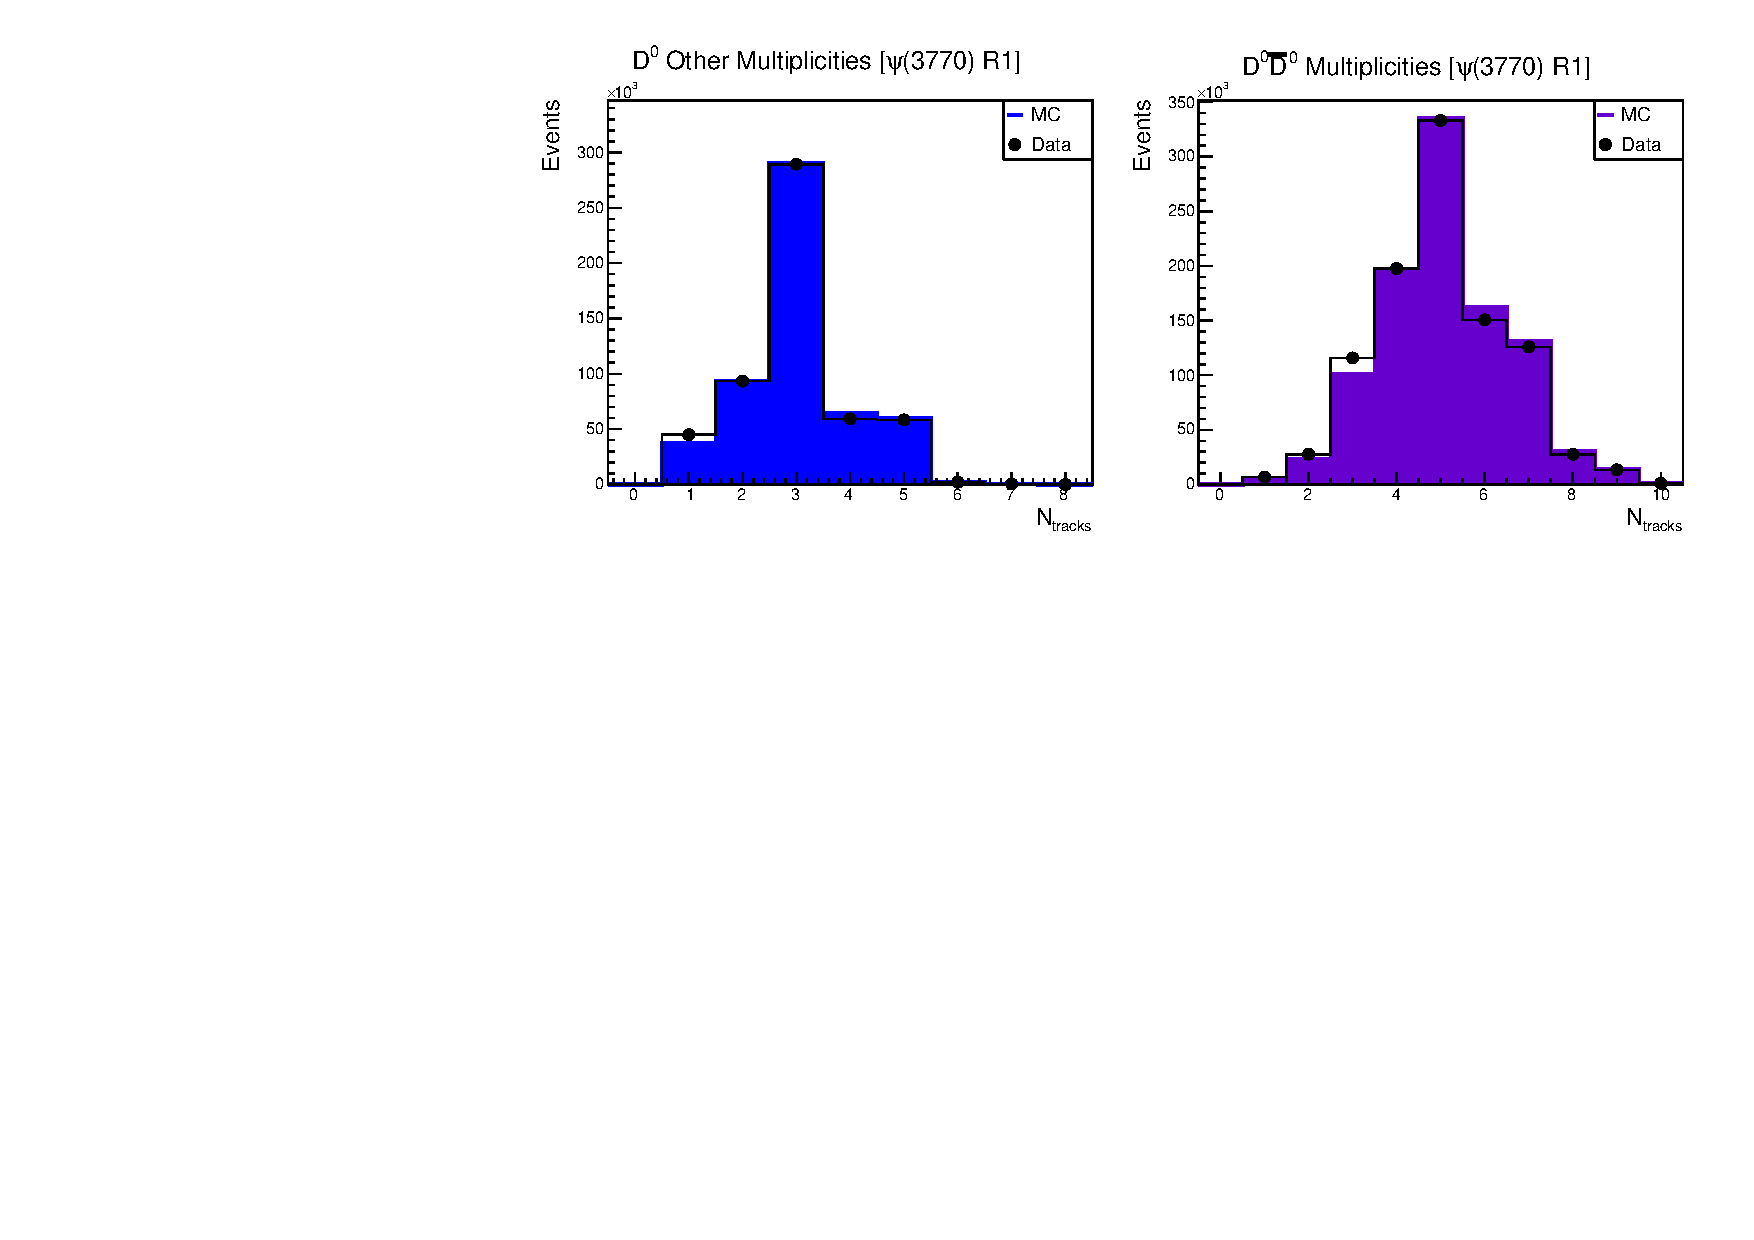
\includegraphics[width=\textwidth]{../figures/plots/DD_corr_plots/DD_psipp_D0D0bar_R1.pdf}
\end{figure}
\vspace{-0.6cm}
\begin{figure}
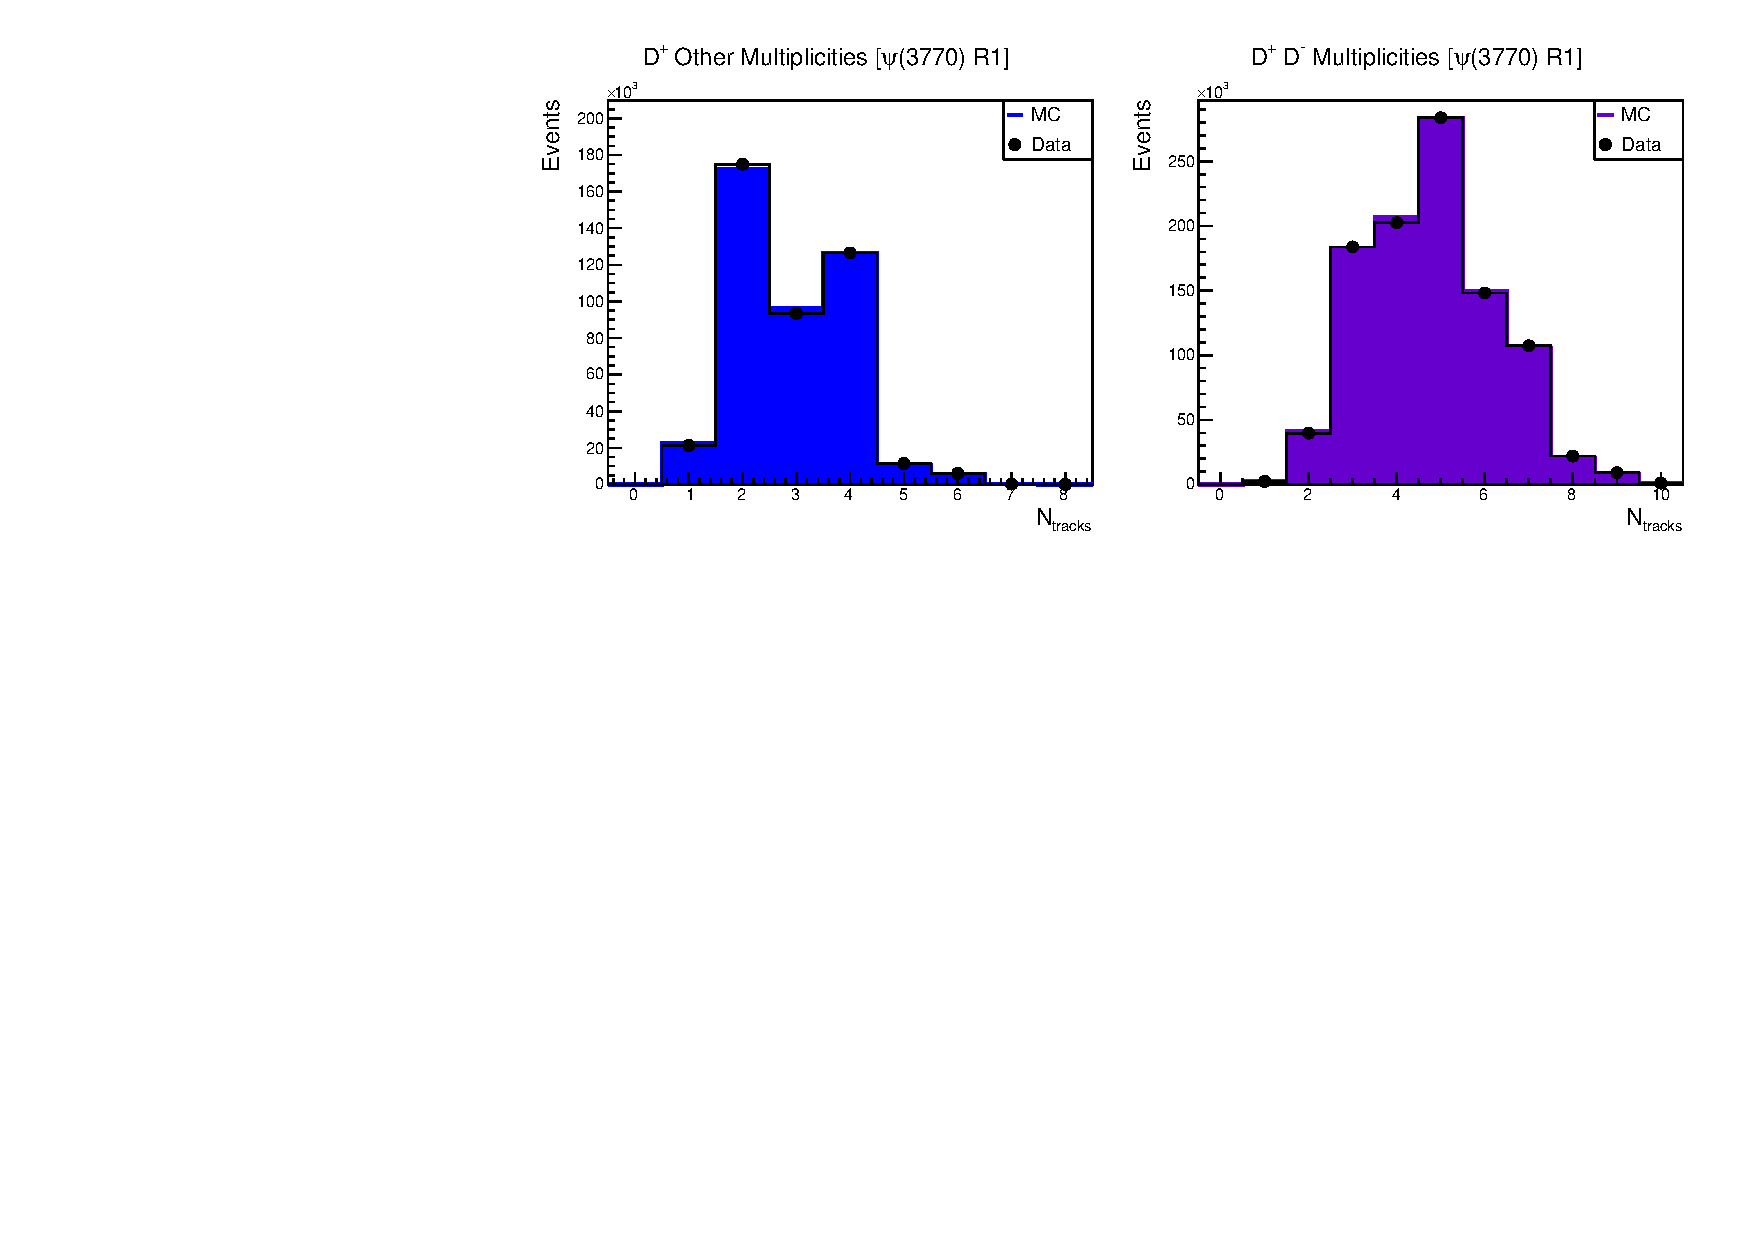
\includegraphics[width=\textwidth]{../figures/plots/DD_corr_plots/DD_psipp_DpDm_R1.pdf}
\end{figure}

\end{columns}
}

\addframe{Hadronic Counts - $\psipp$ (R1)}{

\begin{table}
\footnotesize
\centering
\renewcommand\arraystretch{1.0}
\begin{tabular}{c|r|r@{$\; \pm \;$}r r@{$\; \pm \;$}r r@{$\; \pm \;$}r}
\hline
\multicolumn{8}{c}{$\psipp$ (R1) Reconstruction} \\
\hline
Sample & $\sigma$ [\si{\nb}] & \multicolumn{2}{c}{$\effmc$ (SHAD) [\%]} & \multicolumn{2}{c}{$\effmc$ (LHAD) [\%]} & \multicolumn{2}{c}{$\effmc$ (THAD) [\%]} \\
\hline
$\DO\aDO$ & 3.615 & 73.9324 & 0.0142 & 79.8496 & 0.0147 & 60.3601 & 0.0128 \\
$\Dp\Dm$  & 2.830 & 61.4048 & 0.0146 & 68.8212 & 0.0154 & 49.4007 & 0.0131 \\
$\tautau$ & 2.652 & 12.7566 & 0.0253 & 28.0142 & 0.0374 &  9.8776 & 0.0222 \\
$\yjpsi$  & 0.986 & 46.6185 & 0.0206 & 56.2494 & 0.0227 & 34.7544 & 0.0178 \\
$\ypsip$  & 3.009 & 63.2551 & 0.0137 & 69.9696 & 0.0144 & 51.5643 & 0.0123 \\
\hline          
\end{tabular}
\end{table}

\begin{table}
\footnotesize
\centering
\renewcommand\arraystretch{1.0}
\begin{tabular}{c|r@{$\; \pm \;$}r r@{$\; \pm \;$}r r@{$\; \pm \;$}r}
\hline
\multicolumn{7}{c}{$\psipp$ (R1) Results} \\
\hline
Sample & \multicolumn{2}{c}{$\Nhad$ (SHAD)} & \multicolumn{2}{c}{$\Nhad$ (LHAD)} & \multicolumn{2}{c}{$\Nhad$ (THAD)} \\
\hline
Data             & 15694505 &  3962 & 17722728 &  4210 & 12580701 &  3547 \\
$\qqbar^\dagger$ &  8522688 & 71353 &  9330411 & 76320 &  6789405 & 61599 \\
$\DO\aDO$        &  2477345 &   534 &  2675620 &   560 &  2022561 &   473 \\
$\Dp\Dm$         &  1610764 &   414 &  1805311 &   442 &  1295875 &   366 \\
$\tautau$        &   313542 &   622 &   688559 &   922 &   242781 &   547 \\
$\yjpsi$         &   425891 &   193 &   513875 &   213 &   317504 &   166 \\
$\ypsip$         &  1764254 &   419 &  1951528 &   445 &  1438185 &   372 \\
\hline                                                    
Hadrons          &   490569 & 71795 &   658730 & 76807 &   401064 & 61995 \\
\hline
\end{tabular}
\end{table}
}

\addframe{Initial Exploration of $\psipp$ Data}{
\additem{Convert hadronic signal to $\nonDDbar$ cross section 
\additem{Assume efficiency is similar to that for $\ypsip$ decays}
}
\addcenter{$\xsecpsipptononDDbar = \frac{ N_{\nonDDbar} }{ \epsilon_{\nonDDbar} \times \lum }$}

\vspace{-0.5cm}

\begin{table}
\footnotesize
\centering
\renewcommand\arraystretch{1.0}
\begin{tabular}{c|r@{$\; \pm \;$}r r@{$\; \pm \;$}r r@{$\; \pm \;$}r}
\hline
Sample & \multicolumn{2}{c}{$\sigma_{\nonDDbar}$ (SHAD)} & \multicolumn{2}{c}{$\sigma_{\nonDDbar}$ (LHAD)} & \multicolumn{2}{c}{$\sigma_{\nonDDbar}$ (THAD)} \\[1pt]
\hline
$\psipp$ (R1) & 0.9892 & 0.1219 & 1.1679 & 0.1179 & 0.9925 & 0.1291 \\
$\psipp$ (R2) & 1.0877 & 0.1224 & 1.2926 & 0.1183 & 1.1142 & 0.1298 \\
\hline                                                    
Lum. Weighted & 1.0563 & 0.1223 & 1.2528 & 0.1182 & 1.0754 & 0.1296 \\ 
\hline
\end{tabular}
\end{table}

\vspace{-0.3cm}
\additem{Likely overestimated due to assumption of Breit-Wigner for $\psip$}

\additem{Convert cross section to branching fraction using $\DDbar$ measurements
\addcenter{$\BFpsipptononDDbar = \frac{ \xsecpsipptononDDbar }{ \xsecpsipptoDDbar + \xsecpsipptononDDbar }$}
}
\addcenter{\textbf{Begin exploratory analysis - NOT OFFICIAL MEASUREMENTS}}
}

\addframe{Investigation I: Standard Breit-Wigner for $\psip$}{

\begin{columns}
\column{0.4\textwidth}
\vspace{-0.6cm}
\additem{$\psip$ calculated as standard Breit-Wigner}

\additem{Significant drop in last point of efficiency ratio}

\additem{Upper bound for branching fraction}

\column{0.6\textwidth}
\vspace{-0.6cm}
\begin{figure}
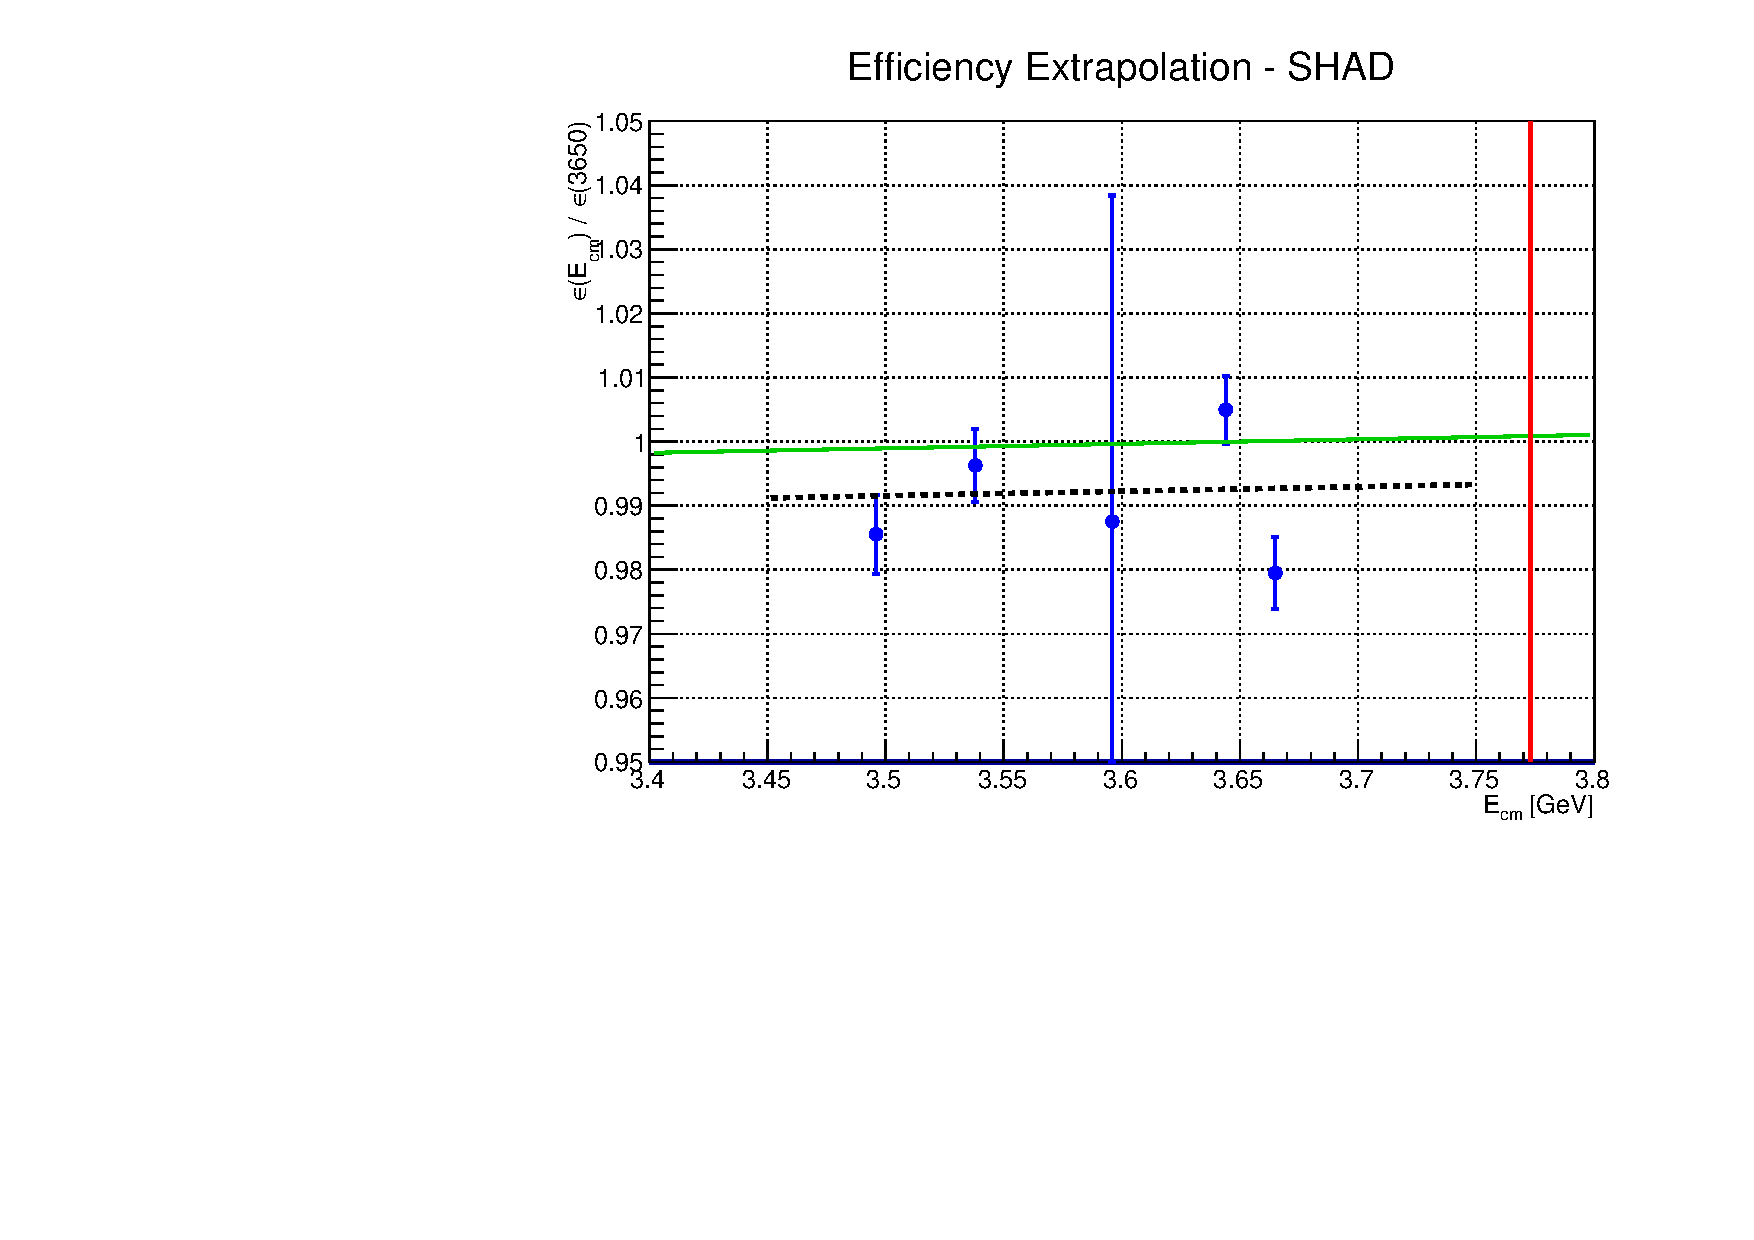
\includegraphics[width=\textwidth]{../figures/plots/SHAD_psip_BW.pdf}
\end{figure}

\end{columns}

\begin{table}
\footnotesize
\centering
\renewcommand\arraystretch{1.0}
\begin{tabular}{c|r@{$\; \pm \;$}r r@{$\; \pm \;$}r r@{$\; \pm \;$}r}
\hline
Sample & \multicolumn{2}{c}{$\Gamma_{\nonDDbar}$ (SHAD)} & \multicolumn{2}{c}{$\Gamma_{\nonDDbar}$ (LHAD)} & \multicolumn{2}{c}{$\Gamma_{\nonDDbar}$ (THAD)} \\[1pt]
\hline
$\psipp$ (R1) & 0.1331 & 0.0183 & 0.1534 & 0.0185 & 0.1334 & 0.0190 \\
$\psipp$ (R2) & 0.1444 & 0.0186 & 0.1671 & 0.0189 & 0.1474 & 0.0193 \\
\hline                                                    
Lum. Weighted & 0.1408 & 0.0185 & 0.1627 & 0.0187 & 0.1430 & 0.0192 \\ 
\hline
\end{tabular}
\end{table}

}

\addframe{Investigation II: Continuum Ratio Estimation}{

\begin{columns}
\column{0.4\textwidth}
\vspace{-0.6cm}
\additem{$\psip$ approximated by}
\addcenter{$\frac{ \sigma_{\text{res}} }{ \sigma_{\text{cont}}(\Ecm) } = \frac{ \sqrt{2\pi} \; (M_{\text{res}} - \Ecm)^2 }{ \Gamma_{\text{res}} \times \delta_{\Ecm}}$}
\additem{Use $\sigma_{\psip}$ from BESIII
\additem{$\delta_{\Ecm} \approx \SI{1.5}{\MeV}$}
}
\additem{Estimated value for branching fraction}

\column{0.6\textwidth}
\vspace{-0.6cm}
\begin{figure}
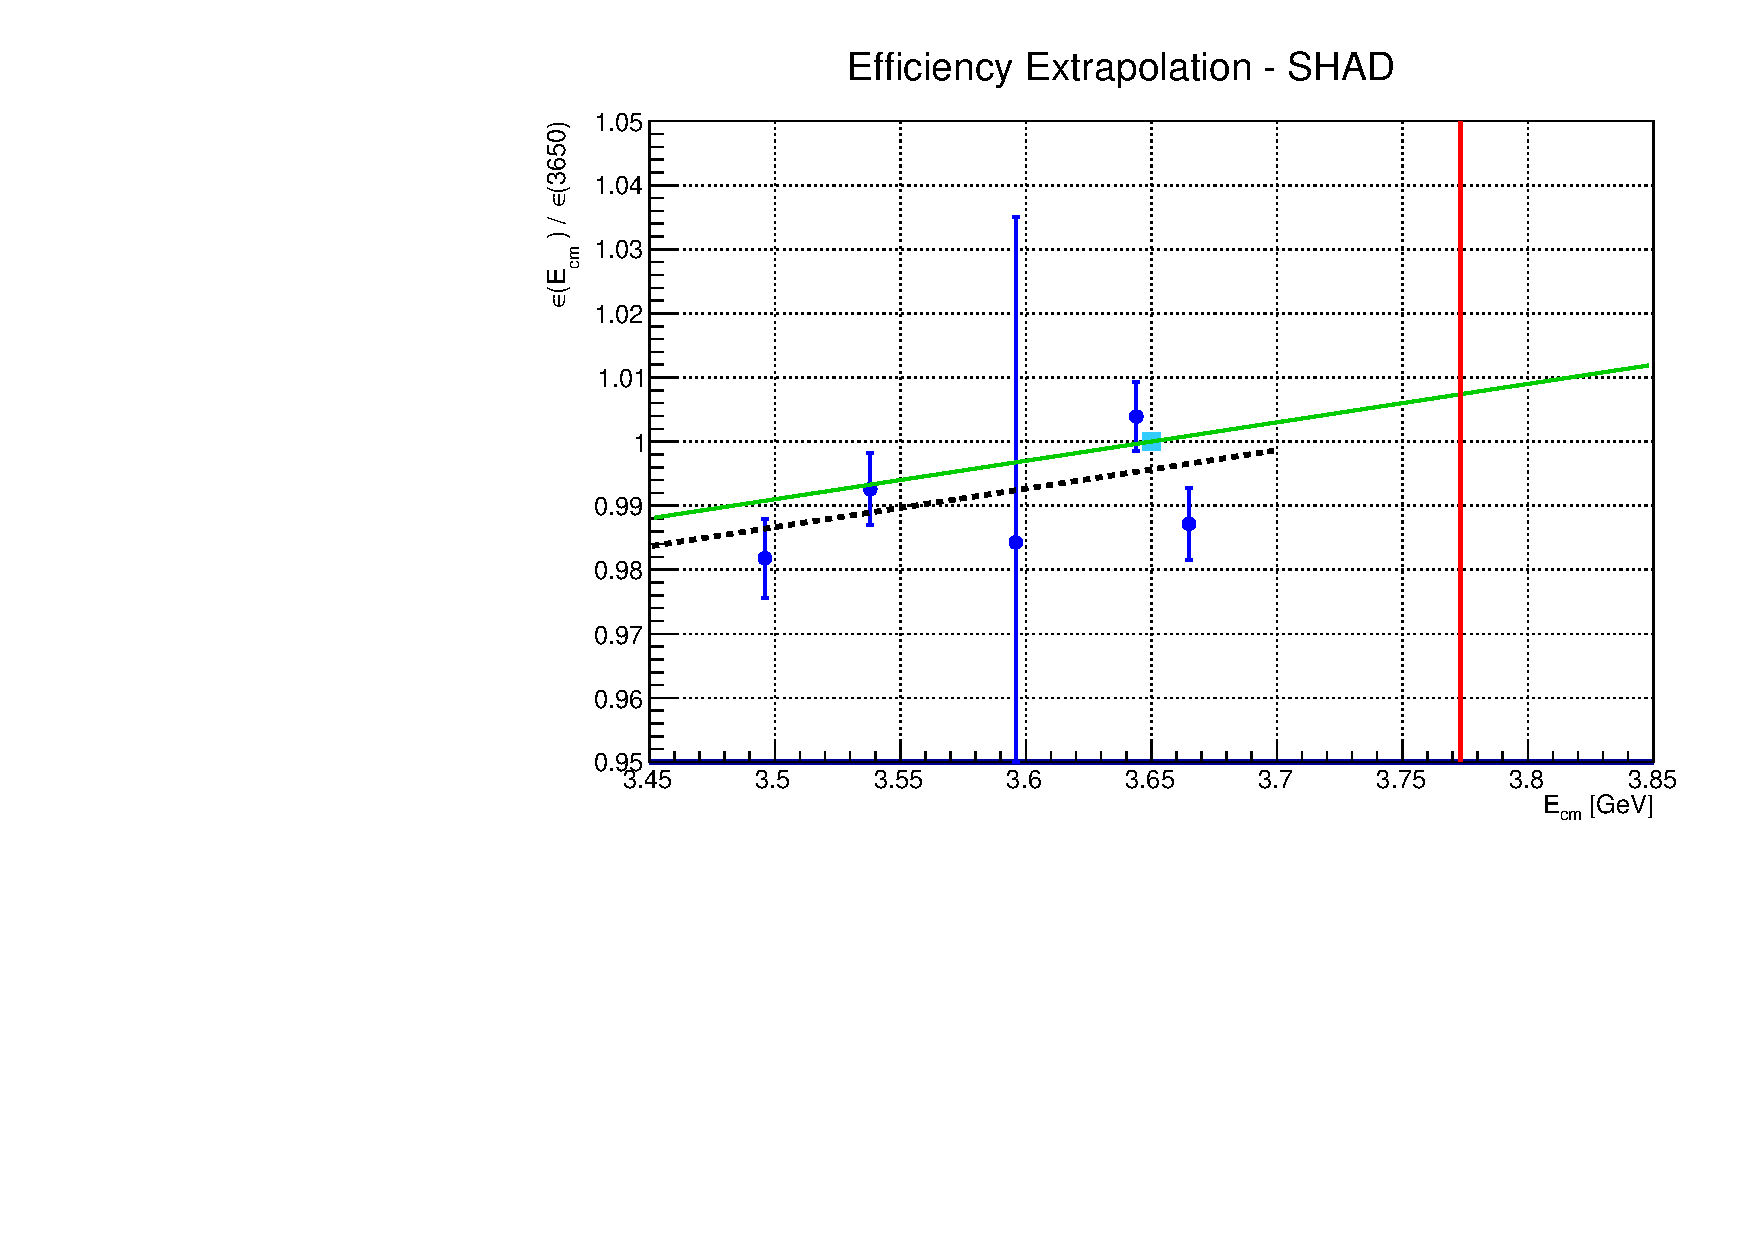
\includegraphics[width=\textwidth]{../figures/plots/SHAD_psip_calc.pdf}
\end{figure}

\end{columns}

\begin{table}
\footnotesize
\centering
\renewcommand\arraystretch{1.0}
\begin{tabular}{c|r@{$\; \pm \;$}r r@{$\; \pm \;$}r r@{$\; \pm \;$}r}
\hline
Sample & \multicolumn{2}{c}{$\Gamma_{\nonDDbar}$ (SHAD)} & \multicolumn{2}{c}{$\Gamma_{\nonDDbar}$ (LHAD)} & \multicolumn{2}{c}{$\Gamma_{\nonDDbar}$ (THAD)} \\[1pt]
\hline
$\psipp$ (R1) & 0.1149 & 0.0180 & 0.1361 & 0.0181 & 0.1152 & 0.0188 \\
$\psipp$ (R2) & 0.1267 & 0.0183 & 0.1504 & 0.0185 & 0.1297 & 0.0190 \\
\hline                                                    
Lum. Weighted & 0.1230 & 0.0182 & 0.1458 & 0.0183 & 0.1251 & 0.0190 \\ 
\hline
\end{tabular}
\end{table}

}

\addframe{Investigation III: No $\psip$ Contribution}{

\begin{columns}
\column{0.4\textwidth}
\vspace{-0.6cm}
\additem{$\psip$ ignored}

\additem{Inaccurate assumption}

\additem{Lower bound for branching fraction}

\column{0.6\textwidth}
\vspace{-0.6cm}
\begin{figure}
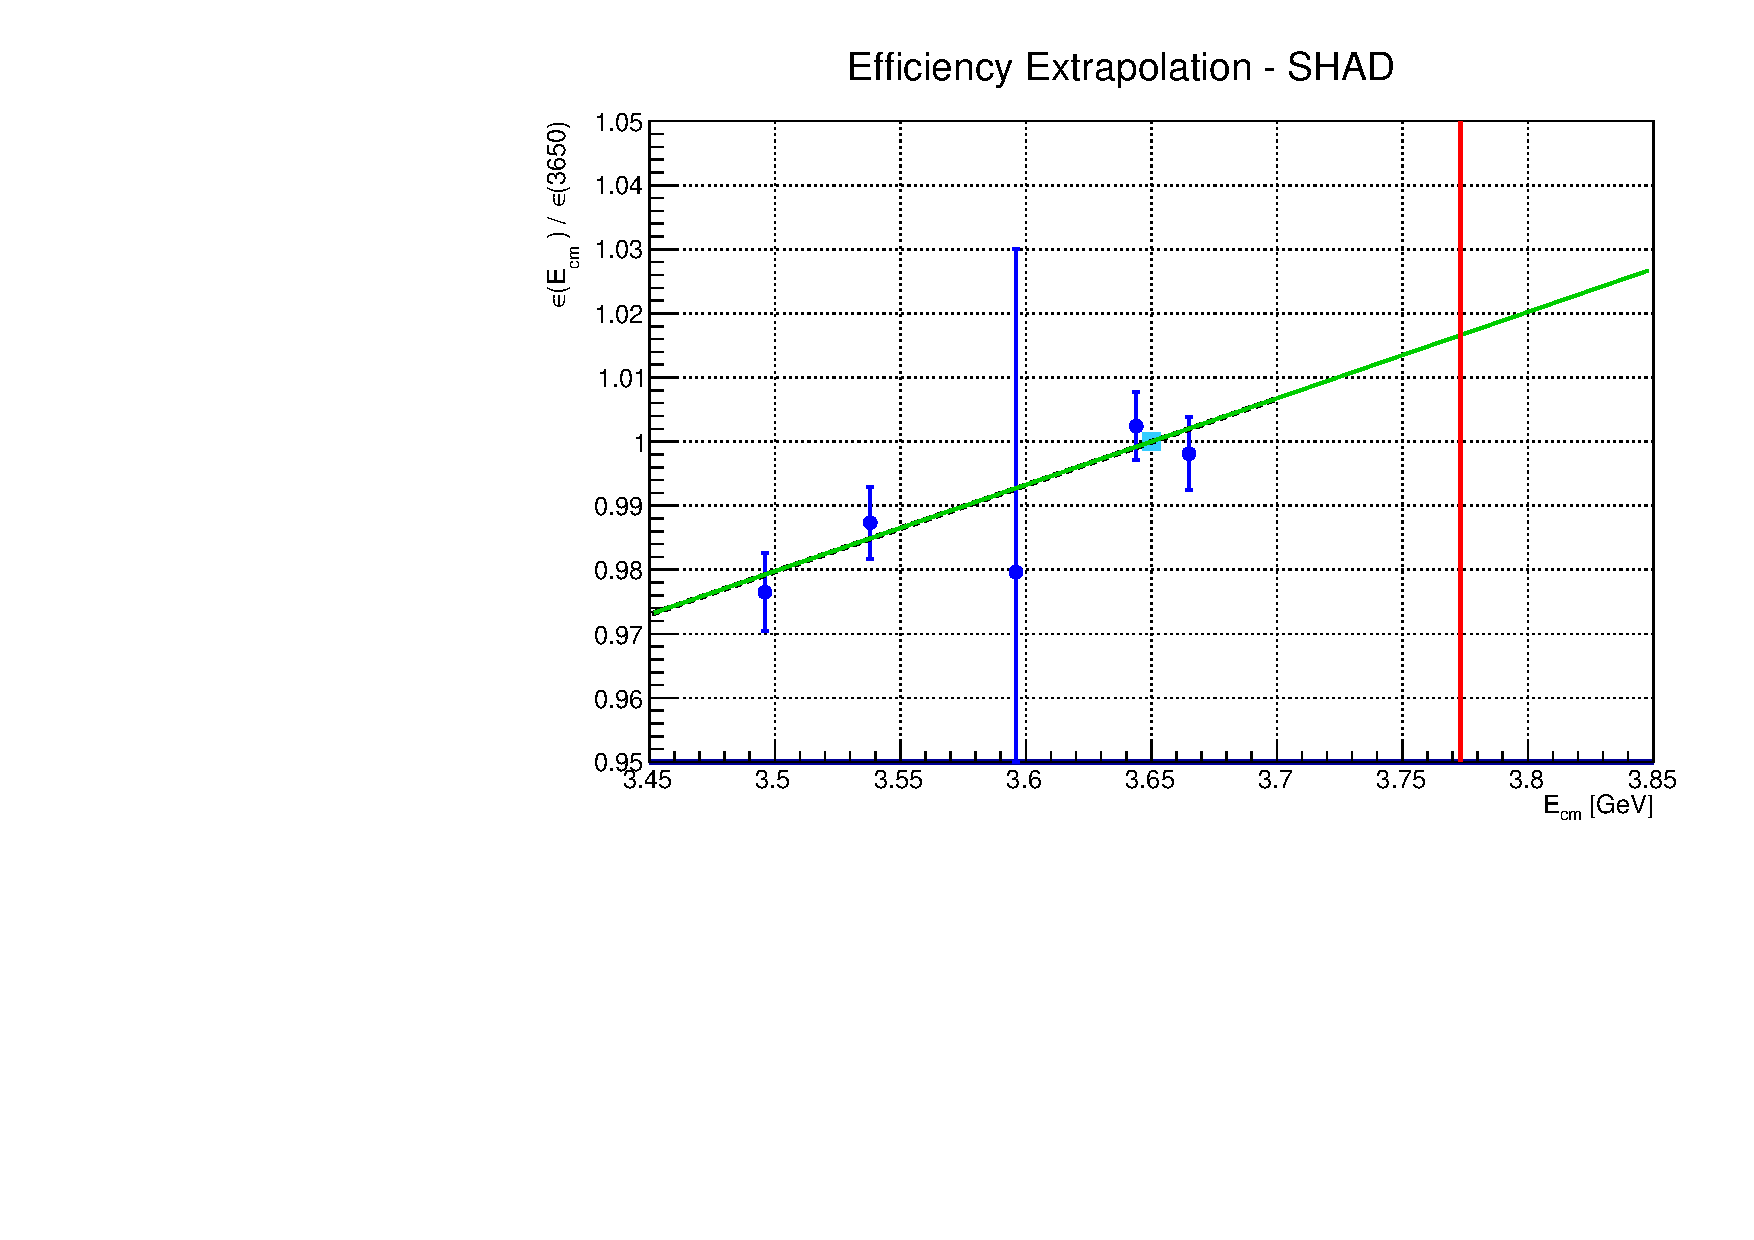
\includegraphics[width=\textwidth]{../figures/plots/SHAD_psip_none.pdf}
\end{figure}

\end{columns}

\begin{table}
\footnotesize
\centering
\renewcommand\arraystretch{1.0}
\begin{tabular}{c|r@{$\; \pm \;$}r r@{$\; \pm \;$}r r@{$\; \pm \;$}r}
\hline
Sample & \multicolumn{2}{c}{$\Gamma_{\nonDDbar}$ (SHAD)} & \multicolumn{2}{c}{$\Gamma_{\nonDDbar}$ (LHAD)} & \multicolumn{2}{c}{$\Gamma_{\nonDDbar}$ (THAD)} \\[1pt]
\hline
$\psipp$ (R1) & 0.0876 & 0.0178 & 0.1102 & 0.0176 & 0.0878 & 0.0187 \\
$\psipp$ (R2) & 0.1002 & 0.0180 & 0.1254 & 0.0179 & 0.1033 & 0.0188 \\
\hline                                                    
Lum. Weighted & 0.0962 & 0.0179 & 0.1205 & 0.0178 & 0.0983 & 0.0188 \\
 \hline
\end{tabular}
\end{table}

}

\addframe{Inclusive Cross Section for Scan Data}{
\vspace{-0.3cm}
\additem{Inclusive hadronic cross section useful for analyses in $\psipp$ region}
\vspace{-0.3cm}
\begin{figure}
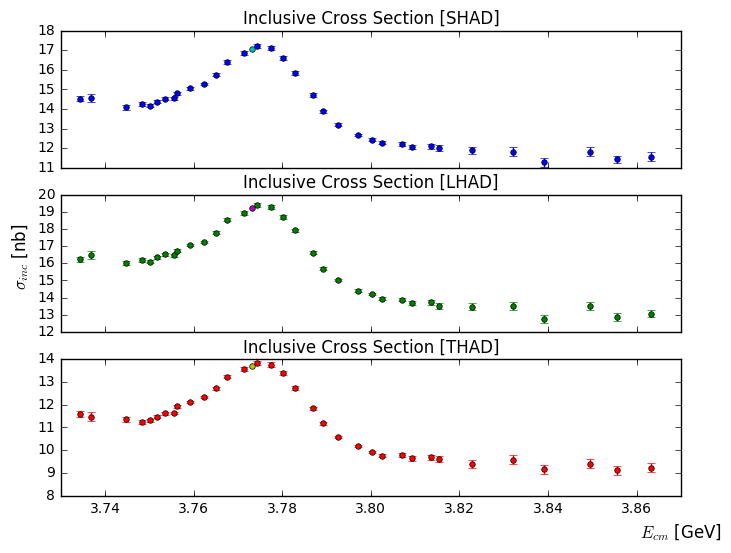
\includegraphics[width=0.8\textwidth]{../figures/plots/xsec_inclusive_scan.png}
\end{figure}

}

\addframe{$\NonDDbar$ Cross Section for Scan Data}{
\vspace{-0.5cm}
\begin{figure}
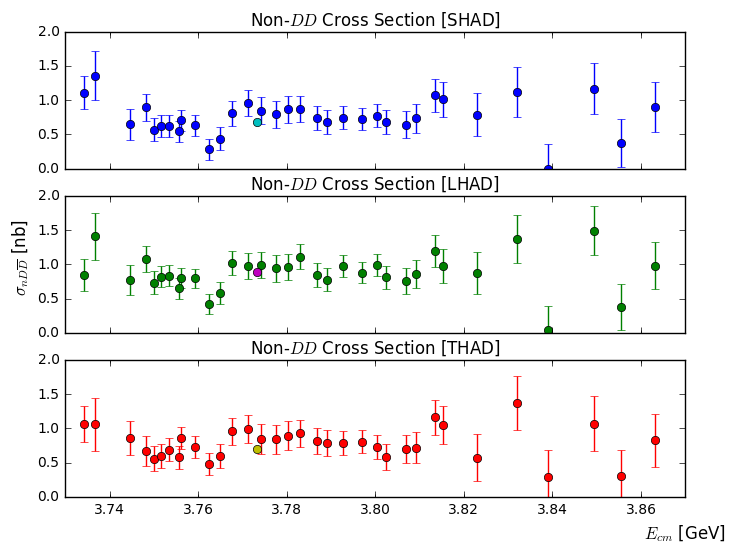
\includegraphics[width=0.88\textwidth]{../figures/plots/xsec_nonDDbar_scan.png}
\end{figure}
}
\addframe{$\NonDDbar$ Branching Fraction for Scan Data}{
\vspace{-0.5cm}
\begin{figure}
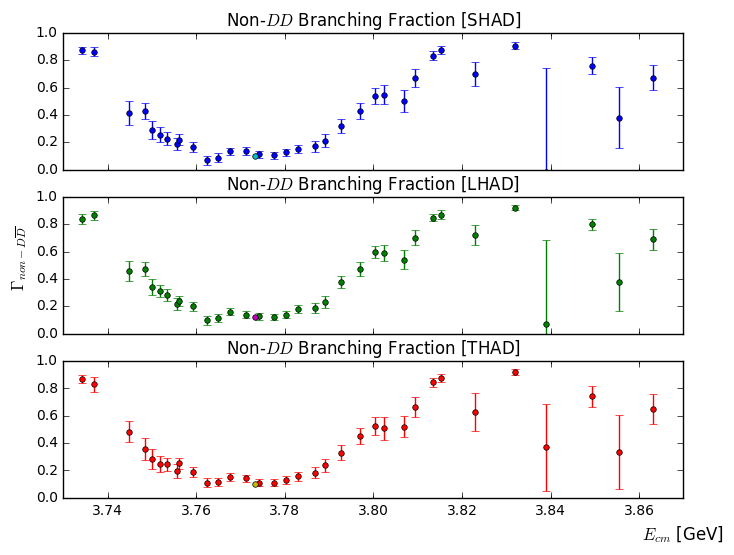
\includegraphics[width=0.88\textwidth]{../figures/plots/bf_nonDDbar_scan.png}
\end{figure}

}


\sectionframe{Conclusion}

\addframe{Conclusion}{
Show overview of measurements for $\DDbar$ cross section and $\nonDDbar$ branching fraction

List results of parameters for $\psipp$

List branching fraction range for $\nonDDbar$
}


\begin{frame}[c]{}
\linespread{2.5}
\begin{block}{$\;$}
\begin{center}
{\Huge Backup Slides}
\end{center}
\end{block}
\end{frame}

\addframe{Monte Carlo Generators}{

\additem{KKMC
\additem{Used to model electroweak interactions: $\ee \rightarrow \ffbar + (n)\gamma$ \\
\quad {\footnotesize $\fermion = \{\lmu, \; \ltau, \; \qup, \; \qdown, \; \qstrange, \; \qcharm, \; \qbottom \}$ and $(n)\gamma$ = (additional photons)}
}
\additem{Decays $\ffbar$ pair based on involved fermions (TAUOLA, PYTHIA)}
\additem{Takes into account initial- and final-state radiation (ISR / FSR)
\additem{For resonances, only handles ISR, then passes off $\photon^*$ to BesEvtGen}
}
}

\additem{BesEvtGen
\additem{Handles resonance decay as well as radiative effects
\additem{Reduced $\Ecm$ such that only lower mass resonances can be produced}
}
}

\additem{Babayaga
\additem{Used to model QED processes: $\ee \rightarrow \{\ee, \; \mumu, \; \yy\}$}
\additem{Very accurate results; estimated theoretical uncertainty of \SI{0.1}{\%}
\additem{High precision required for determination of integrated luminosity}
}
}
}

\addframe{Selection Cuts}{

\begin{table}[h]
\centering
\begin{tabular}{c| r@{$\; < \;$}l }
\multicolumn{3}{c}{$\pipm$ and $\Kpm$ Selection} \\
\hline
Vertex ($xy$)    & $V_{xy}$ & \pp \SI{1}{\cm} \\
Vertex ($z$)     & $|Vz|$   & \SI{10}{\cm} \\
MDC Angle        & $|\cos\theta|$ & 0.93 \\
Pion Probability & \multicolumn{2}{c}{ $\pp P(\pi) > 0, \quad P(\pi) > P(K)$ } \\
Kaon Probability & \multicolumn{2}{c}{ $    P(K)   > 0, \quad P(K) > P(\pi)$ } \\
\hline
\end{tabular}
\end{table}

\begin{table}[h]
\centering
\begin{tabular}{c|c r}
\multicolumn{3}{c}{$\photon$ Selection} \\
\hline
Min. Energy (Barrel) & $E_{\text{EMC}} > \SI{25}{\MeV}$ & $       (|\cos\theta| < 0.80)$ \\
Min. Energy (Endcap) & $E_{\text{EMC}} > \SI{50}{\MeV}$ & $(0.84 < |\cos\theta| < 0.92)$ \\
TDC Timing & $ (0 \leq t \leq 14) \times \SI{50}{\ns} $ \\ 
\hline
\end{tabular}
\end{table}

\begin{table}[h]
\centering
\begin{tabular}{c|c|c}
& $\piO \rightarrow \yy$ Selection & $\Ks \rightarrow \pip\pim$ Selection \\
\hline
Nominal Mass & $115 < m_{\piO} [\si{\MeV}] < 150$ & $487 < m_{\Ks} [\si{\MeV}] < 511$ \\
Fit Quality  & $\chi^2 < 200$, Converged& $\chi^2 < 100$, Converged \\
\hline
\end{tabular}
\end{table}

}


\addframe{Derivation of $\xsecpsipptoDDbar$}{
\additem{$
\mathcal{F}(x, W^2) = \beta \, x^{\beta - 1} \left[ 1 + \frac{\alpha}{\pi} \left( \frac{\pi^2}{3} - \frac{1}{2} \right) + \frac{3}{4} \beta + \beta^2 \left( \frac{37}{96} - \frac{\pi^2}{12} - \frac{L}{72} \right) \right] = \beta \, x^{\beta - 1} F(W^2), 
\qquad \qquad \qquad \beta = \frac{2 \alpha}{\pi} (L - 1), \qquad L = \log \left( \frac{W^2}{m_e^2} \right)
$}
% , \qquad \beta_D = \sqrt{1 - \frac{ 4 m_D^2 }{ W^2 } }$}
% \additem{$F_D(W) = F_D^{\text{NR}}(W) + \sum\limits_r F^{R_r}_D(W) \, e^{i \phi_r }$}
}

\addframe{$\sCP$ Violation Correction}{
Quickly list process of correcting for $\sCP$
}

\addframe{Hadronic Selection Event Cuts}{
Show charged / neutral / QED cut tables
}

\addframe{Hadronic Selection Group Cuts}{
Show SHAD, LHAD, and THAD cut tables
}

\end{document} 
